% Options for packages loaded elsewhere
\PassOptionsToPackage{unicode}{hyperref}
\PassOptionsToPackage{hyphens}{url}
%
\documentclass[
]{book}
\usepackage{lmodern}
\usepackage{amsmath}
\usepackage{ifxetex,ifluatex}
\ifnum 0\ifxetex 1\fi\ifluatex 1\fi=0 % if pdftex
  \usepackage[T1]{fontenc}
  \usepackage[utf8]{inputenc}
  \usepackage{textcomp} % provide euro and other symbols
  \usepackage{amssymb}
\else % if luatex or xetex
  \usepackage{unicode-math}
  \defaultfontfeatures{Scale=MatchLowercase}
  \defaultfontfeatures[\rmfamily]{Ligatures=TeX,Scale=1}
\fi
% Use upquote if available, for straight quotes in verbatim environments
\IfFileExists{upquote.sty}{\usepackage{upquote}}{}
\IfFileExists{microtype.sty}{% use microtype if available
  \usepackage[]{microtype}
  \UseMicrotypeSet[protrusion]{basicmath} % disable protrusion for tt fonts
}{}
\makeatletter
\@ifundefined{KOMAClassName}{% if non-KOMA class
  \IfFileExists{parskip.sty}{%
    \usepackage{parskip}
  }{% else
    \setlength{\parindent}{0pt}
    \setlength{\parskip}{6pt plus 2pt minus 1pt}}
}{% if KOMA class
  \KOMAoptions{parskip=half}}
\makeatother
\usepackage{xcolor}
\IfFileExists{xurl.sty}{\usepackage{xurl}}{} % add URL line breaks if available
\IfFileExists{bookmark.sty}{\usepackage{bookmark}}{\usepackage{hyperref}}
\hypersetup{
  pdftitle={Child Development with the D-score: Turning Milestones into Measurement},
  pdfauthor={Authors: Stef van Buuren \& Iris Eekhout},
  hidelinks,
  pdfcreator={LaTeX via pandoc}}
\urlstyle{same} % disable monospaced font for URLs
\usepackage{longtable,booktabs}
\usepackage{calc} % for calculating minipage widths
% Correct order of tables after \paragraph or \subparagraph
\usepackage{etoolbox}
\makeatletter
\patchcmd\longtable{\par}{\if@noskipsec\mbox{}\fi\par}{}{}
\makeatother
% Allow footnotes in longtable head/foot
\IfFileExists{footnotehyper.sty}{\usepackage{footnotehyper}}{\usepackage{footnote}}
\makesavenoteenv{longtable}
\usepackage{graphicx}
\makeatletter
\def\maxwidth{\ifdim\Gin@nat@width>\linewidth\linewidth\else\Gin@nat@width\fi}
\def\maxheight{\ifdim\Gin@nat@height>\textheight\textheight\else\Gin@nat@height\fi}
\makeatother
% Scale images if necessary, so that they will not overflow the page
% margins by default, and it is still possible to overwrite the defaults
% using explicit options in \includegraphics[width, height, ...]{}
\setkeys{Gin}{width=\maxwidth,height=\maxheight,keepaspectratio}
% Set default figure placement to htbp
\makeatletter
\def\fps@figure{htbp}
\makeatother
\setlength{\emergencystretch}{3em} % prevent overfull lines
\providecommand{\tightlist}{%
  \setlength{\itemsep}{0pt}\setlength{\parskip}{0pt}}
\setcounter{secnumdepth}{5}
\usepackage{booktabs}
\usepackage{longtable}
\usepackage{array}
\usepackage{multirow}
\usepackage{wrapfig}
\usepackage{float}
\usepackage{colortbl}
\usepackage{pdflscape}
\usepackage{tabu}
\usepackage{threeparttable}
\usepackage{threeparttablex}
\usepackage[normalem]{ulem}
\usepackage{makecell}
\usepackage{xcolor}
\usepackage{multicol}
\usepackage{hhline}
\usepackage{hyperref}
\ifluatex
  \usepackage{selnolig}  % disable illegal ligatures
\fi
\newlength{\cslhangindent}
\setlength{\cslhangindent}{1.5em}
\newlength{\csllabelwidth}
\setlength{\csllabelwidth}{3em}
\newenvironment{CSLReferences}[3] % #1 hanging-ident, #2 entry spacing
 {% don't indent paragraphs
  \setlength{\parindent}{0pt}
  % turn on hanging indent if param 1 is 1
  \ifodd #1 \everypar{\setlength{\hangindent}{\cslhangindent}}\ignorespaces\fi
  % set entry spacing
  \ifnum #2 > 0
  \setlength{\parskip}{#2\baselineskip}
  \fi
 }%
 {}
\usepackage{calc}
\newcommand{\CSLBlock}[1]{#1\hfill\break}
\newcommand{\CSLLeftMargin}[1]{\parbox[t]{\csllabelwidth}{#1}}
\newcommand{\CSLRightInline}[1]{\parbox[t]{\linewidth - \csllabelwidth}{#1}}
\newcommand{\CSLIndent}[1]{\hspace{\cslhangindent}#1}

\title{Child Development with the D-score: Turning Milestones into Measurement}
\author{Authors: Stef van Buuren \& Iris Eekhout}
\date{}

\begin{document}
\maketitle

{
\setcounter{tocdepth}{1}
\tableofcontents
}
\hypertarget{frontmatter}{%
\chapter*{Frontmatter}\label{frontmatter}}
\addcontentsline{toc}{chapter}{Frontmatter}

\newpage

\hypertarget{ch:history}{%
\chapter{Short history}\label{ch:history}}

The measurement of child development has quite an extensive history. This section

\begin{itemize}
\tightlist
\item
  reviews definitions of child development (\ref{sec:definitions})
\item
  discusses concepts in the nature of child development (\ref{sec:theories})
\item
  shows a classic example of motor measurements (\ref{sec:motorexample})
\item
  summarizes typical questions whose answers need proper measurements (\ref{sec:questions})
\end{itemize}

\hypertarget{sec:definitions}{%
\section{What is child development?}\label{sec:definitions}}

In contrast to concepts like height or temperature, it is unclear what exactly constitutes child development. \protect\hyperlink{ref-shirley1931}{Shirley} (\protect\hyperlink{ref-shirley1931}{1931}) executed one of the first rigorous studies in the field with the explicit aim

\begin{quote}
that the many aspects of development, anatomical, physical, motor, intellectual, and emotional, be studied simultaneously.
\end{quote}

Shirley gave empirical definitions of each of these domains of development.

\begin{figure}

{\centering \includegraphics[width=1\linewidth]{fig/firsttwoyearsast011504} 

}

\caption{Gross motor development as a sequence of milestones. Source: \protect\hyperlink{ref-shirley1933}{Shirley} (\protect\hyperlink{ref-shirley1933}{1933}), with permission.}\label{fig:shirleyplot}
\end{figure}



Certain domains advance through a fixed sequence. Figure \ref{fig:shirleyplot} illustrates the various stages needed for going from a \emph{fetal posture} to \emph{walking alone}. The ages are indicative of when these events happen, but there is a considerable variation in timing between infants.

\protect\hyperlink{ref-gesell1943}{Gesell} (\protect\hyperlink{ref-gesell1943}{1943}) (p.~88) formulated the following definition of development:

\begin{quote}
Development is a continuous process that proceeds stage by stage in an orderly sequence.
\end{quote}

Gesell's definition emphasizes that development is a continuous process. The stages are useful as indicators to infer the level of maturity but are of limited interest by themselves.

\protect\hyperlink{ref-liebert1974}{Liebert, Poulos, and Strauss} (\protect\hyperlink{ref-liebert1974}{1974}) (p.~5) emphasized that development is not a phenomenon that unfolds in isolation.

\begin{quote}
Development refers to a process in growth and capability over time, as a function of both maturation and interaction with the environment.
\end{quote}

\protect\hyperlink{ref-cameron2012}{Cameron and Bogin} (\protect\hyperlink{ref-cameron2012}{2012}) (p.~11) defined an endpoint of development, as follows:

\begin{quote}
``Growth'' is defined as an increase in size, while ``maturity'' or ``development'' is an increase in functional ability\ldots The endpoint of maturity is when a human is functionally able to procreate successfully \ldots{} not just biological maturity but also behavioural and perhaps social maturity.
\end{quote}

\protect\hyperlink{ref-berk2013}{Berk} (\protect\hyperlink{ref-berk2013}{2011}) (p.~30) presented a dynamic systems perspective on child development as follows:

\begin{quote}
Development cannot be characterized as a single line of change, and is more like a web of fibres branching out in many directions, each representing a different skill area that may undergo both continuous and stagewise transformation.
\end{quote}

There are many more definitions of child development. The ones described here illustrate the main points of view in the field.

\hypertarget{sec:theories}{%
\section{Theories of child development}\label{sec:theories}}

The field of child development is vast and spans multiple academic disciplines. This short overview, therefore, cannot do justice to the enormous richness. Readers new to the field might orient themselves by browsing through an introductory academic titles (\protect\hyperlink{ref-santrock2010}{Santrock 2011}; \protect\hyperlink{ref-berk2013}{Berk 2011}), or by searching for the topic of interest in an encyclopedia, e.g., \protect\hyperlink{ref-salkind2002}{Salkind} (\protect\hyperlink{ref-salkind2002}{2002}).

The introductions by \protect\hyperlink{ref-santrock2010}{Santrock} (\protect\hyperlink{ref-santrock2010}{2011}) and \protect\hyperlink{ref-berk2013}{Berk} (\protect\hyperlink{ref-berk2013}{2011}) both distinguish major theories in child development according to how each answer to following three questions:

\hypertarget{continuous-or-discontinuous}{%
\subsection{Continuous or discontinuous?}\label{continuous-or-discontinuous}}

Does development evolve gradually as a continuous process or are there qualitatively distinct stages, with jumps occurring from one step to another?

Many stage-based theories of human development have been proposed over the years: social and emotional development by psycho-sexual stages introduced by Freud and furthered by Erikson (\protect\hyperlink{ref-erikson1963}{Erikson 1963}), Kohlberg's six stages of moral development (\protect\hyperlink{ref-kohlberg1984}{Kohlberg 1984}) and Piaget's cognitive development theory (\protect\hyperlink{ref-piaget1969}{Piaget and Inhelder 1969}). Piaget distinguishes four main periods throughout childhood. The first period, the \emph{sensorimotor period} (approximately 0-2 years), is subdivided into six stages. When taken together, these six stages describe ``the road to conceptual thought.'' Piaget's stages are qualitatively different and aim to unravel the mechanism involved in intellectual development.

On the other hand, Gesell and others emphasize development as a continuous process. \protect\hyperlink{ref-gesell1943}{Gesell} (\protect\hyperlink{ref-gesell1943}{1943}) (p.~88) says:

\begin{quote}
A stage represents a degree or level of maturity in the cycle of development. A stage is simply a passing moment, while development, like time, keeps marching on.
\end{quote}

\hypertarget{one-course-or-multiple-parallel-tracks}{%
\subsection{One course or multiple parallel tracks?}\label{one-course-or-multiple-parallel-tracks}}

Stage theorists assume that children progress sequentially through the same set of stages. This assumption is also explicit in the work of Gesell.

The ecological and dynamic systems theories view development as continuous, though not necessarily progressing in an orderly fashion, so there may be multiple, parallel ways to reach the same point. The developmental path taken by a given child will depend on the child's unique combination of personal and environmental circumstances, including cultural diversity in development.

\hypertarget{nature-or-nurture}{%
\subsection{Nature or nurture?}\label{nature-or-nurture}}

\begin{figure}

{\centering \includegraphics[width=1\linewidth]{fig/shutterstock_261441989} 

}

\caption{A group of culturally diverse children. Source: Shutterstock, under license.}\label{fig:diverse}
\end{figure}



Figure \ref{fig:diverse} illustrates that children vary in appearance. Are genetic or environmental factors more important for influencing development? Most theories generally acknowledge the role of both but differ in emphasis. In practice, the debate centres on the question of how to explain individual differences.

Maturation is the process of becoming fully developed, much like the natural unfolding of a flower. The process depends on both genetic factors (species, breed) as well as environmental influences (sunlight, water, nutrition). Some theorists emphasize that differences in child development are innate and stable over time, although there may be differences in unfolding speed due to different environments. Others argue that environmental factors drive differences in development between children, and changing these factors could very well impact child development.

Our position in this debate has practical implications. If we believe that differences are natural and stable, then it may not make much sense trying to change the environment, as the impact on development is likely to be small. On the other hand, we may consider developmental potential as evenly distributed, with its expression governed by the environment. In the latter case, improving life circumstances may have substantial pay-offs in terms of better development.

\hypertarget{sec:motorexample}{%
\section{Example of motor development}\label{sec:motorexample}}

\hypertarget{shirleys-motor-data}{%
\subsection{Shirley's motor data}\label{shirleys-motor-data}}

For illustration, we use data on loco-motor development from a classic study on child development among 25 babies. \protect\hyperlink{ref-shirley1931}{Shirley} (\protect\hyperlink{ref-shirley1931}{1931}) collected measurements of the baby's walking ability, starting at ages around 13 weeks, in an ingenious way. The investigator lays out a white paper of twelve inches wide on the floor of the living room, and lightly greases the soles of the baby's feet with olive oil. The baby was invited to ``walk'' on the sheet. Of course, very young infants need substantial assistance. Footprints left were later coloured by graphite and measured. Measurements during the first year were repeated every week or bi-weekly.

\begin{verbatim}
Warning: Warning: fonts used in `flextable` are ignored because the `pdflatex`
engine is used and not `xelatex` or `lualatex`. You can avoid this warning
by using the `set_flextable_defaults(fonts_ignore=TRUE)` command or use a
compatible engine by defining `latex_engine: xelatex` in the YAML header of the
R Markdown document.
\end{verbatim}

\providecommand{\docline}[3]{\noalign{\global\setlength{\arrayrulewidth}{#1}}\arrayrulecolor[HTML]{#2}\cline{#3}}

\setlength{\tabcolsep}{2pt}

\renewcommand*{\arraystretch}{1.5}

\begin{longtable}[c]{cccccc}

\caption{Age at beginning stages of walking (in weeks) for 21 babies. Source: Shirley (1931).}\label{tab:shirley}\\

\hhline{>{\arrayrulecolor[HTML]{666666}\global\arrayrulewidth=2pt}->{\arrayrulecolor[HTML]{666666}\global\arrayrulewidth=2pt}->{\arrayrulecolor[HTML]{666666}\global\arrayrulewidth=2pt}->{\arrayrulecolor[HTML]{666666}\global\arrayrulewidth=2pt}->{\arrayrulecolor[HTML]{666666}\global\arrayrulewidth=2pt}->{\arrayrulecolor[HTML]{666666}\global\arrayrulewidth=2pt}-}

\multicolumn{1}{!{\color[HTML]{000000}\vrule width 0pt}>{}l}{\fontsize{11}{11}\selectfont{\textcolor[HTML]{000000}{Name}}} & \multicolumn{1}{!{\color[HTML]{000000}\vrule width 0pt}>{}l}{\fontsize{11}{11}\selectfont{\textcolor[HTML]{000000}{Sex}}} & \multicolumn{1}{!{\color[HTML]{000000}\vrule width 0pt}>{}r}{\fontsize{11}{11}\selectfont{\textcolor[HTML]{000000}{Stepping}}} & \multicolumn{1}{!{\color[HTML]{000000}\vrule width 0pt}>{}r}{\fontsize{11}{11}\selectfont{\textcolor[HTML]{000000}{Standing}}} & \multicolumn{1}{!{\color[HTML]{000000}\vrule width 0pt}>{}r}{\fontsize{11}{11}\selectfont{\textcolor[HTML]{000000}{Walking with help}}} & \multicolumn{1}{!{\color[HTML]{000000}\vrule width 0pt}>{}r!{\color[HTML]{000000}\vrule width 0pt}}{\fontsize{11}{11}\selectfont{\textcolor[HTML]{000000}{Walking alone}}} \\

\noalign{\global\setlength{\arrayrulewidth}{2pt}}\arrayrulecolor[HTML]{666666}\cline{1-6}

\endfirsthead

\hhline{>{\arrayrulecolor[HTML]{666666}\global\arrayrulewidth=2pt}->{\arrayrulecolor[HTML]{666666}\global\arrayrulewidth=2pt}->{\arrayrulecolor[HTML]{666666}\global\arrayrulewidth=2pt}->{\arrayrulecolor[HTML]{666666}\global\arrayrulewidth=2pt}->{\arrayrulecolor[HTML]{666666}\global\arrayrulewidth=2pt}->{\arrayrulecolor[HTML]{666666}\global\arrayrulewidth=2pt}-}

\multicolumn{1}{!{\color[HTML]{000000}\vrule width 0pt}>{}l}{\fontsize{11}{11}\selectfont{\textcolor[HTML]{000000}{Name}}} & \multicolumn{1}{!{\color[HTML]{000000}\vrule width 0pt}>{}l}{\fontsize{11}{11}\selectfont{\textcolor[HTML]{000000}{Sex}}} & \multicolumn{1}{!{\color[HTML]{000000}\vrule width 0pt}>{}r}{\fontsize{11}{11}\selectfont{\textcolor[HTML]{000000}{Stepping}}} & \multicolumn{1}{!{\color[HTML]{000000}\vrule width 0pt}>{}r}{\fontsize{11}{11}\selectfont{\textcolor[HTML]{000000}{Standing}}} & \multicolumn{1}{!{\color[HTML]{000000}\vrule width 0pt}>{}r}{\fontsize{11}{11}\selectfont{\textcolor[HTML]{000000}{Walking with help}}} & \multicolumn{1}{!{\color[HTML]{000000}\vrule width 0pt}>{}r!{\color[HTML]{000000}\vrule width 0pt}}{\fontsize{11}{11}\selectfont{\textcolor[HTML]{000000}{Walking alone}}} \\

\noalign{\global\setlength{\arrayrulewidth}{2pt}}\arrayrulecolor[HTML]{666666}\cline{1-6}\endhead



\multicolumn{1}{!{\color[HTML]{000000}\vrule width 0pt}>{}l}{\fontsize{11}{11}\selectfont{\textcolor[HTML]{000000}{Martin}}} & \multicolumn{1}{!{\color[HTML]{000000}\vrule width 0pt}>{}l}{\fontsize{11}{11}\selectfont{\textcolor[HTML]{000000}{boy}}} & \multicolumn{1}{!{\color[HTML]{000000}\vrule width 0pt}>{}r}{\fontsize{11}{11}\selectfont{\textcolor[HTML]{000000}{15}}} & \multicolumn{1}{!{\color[HTML]{000000}\vrule width 0pt}>{}r}{\fontsize{11}{11}\selectfont{\textcolor[HTML]{000000}{}}} & \multicolumn{1}{!{\color[HTML]{000000}\vrule width 0pt}>{}r}{\fontsize{11}{11}\selectfont{\textcolor[HTML]{000000}{21}}} & \multicolumn{1}{!{\color[HTML]{000000}\vrule width 0pt}>{}r!{\color[HTML]{000000}\vrule width 0pt}}{\fontsize{11}{11}\selectfont{\textcolor[HTML]{000000}{50}}} \\





\multicolumn{1}{!{\color[HTML]{000000}\vrule width 0pt}>{}l}{\fontsize{11}{11}\selectfont{\textcolor[HTML]{000000}{Carol}}} & \multicolumn{1}{!{\color[HTML]{000000}\vrule width 0pt}>{}l}{\fontsize{11}{11}\selectfont{\textcolor[HTML]{000000}{girl}}} & \multicolumn{1}{!{\color[HTML]{000000}\vrule width 0pt}>{}r}{\fontsize{11}{11}\selectfont{\textcolor[HTML]{000000}{15}}} & \multicolumn{1}{!{\color[HTML]{000000}\vrule width 0pt}>{}r}{\fontsize{11}{11}\selectfont{\textcolor[HTML]{000000}{19}}} & \multicolumn{1}{!{\color[HTML]{000000}\vrule width 0pt}>{}r}{\fontsize{11}{11}\selectfont{\textcolor[HTML]{000000}{37}}} & \multicolumn{1}{!{\color[HTML]{000000}\vrule width 0pt}>{}r!{\color[HTML]{000000}\vrule width 0pt}}{\fontsize{11}{11}\selectfont{\textcolor[HTML]{000000}{50}}} \\





\multicolumn{1}{!{\color[HTML]{000000}\vrule width 0pt}>{}l}{\fontsize{11}{11}\selectfont{\textcolor[HTML]{000000}{Max}}} & \multicolumn{1}{!{\color[HTML]{000000}\vrule width 0pt}>{}l}{\fontsize{11}{11}\selectfont{\textcolor[HTML]{000000}{boy}}} & \multicolumn{1}{!{\color[HTML]{000000}\vrule width 0pt}>{}r}{\fontsize{11}{11}\selectfont{\textcolor[HTML]{000000}{14}}} & \multicolumn{1}{!{\color[HTML]{000000}\vrule width 0pt}>{}r}{\fontsize{11}{11}\selectfont{\textcolor[HTML]{000000}{}}} & \multicolumn{1}{!{\color[HTML]{000000}\vrule width 0pt}>{}r}{\fontsize{11}{11}\selectfont{\textcolor[HTML]{000000}{25}}} & \multicolumn{1}{!{\color[HTML]{000000}\vrule width 0pt}>{}r!{\color[HTML]{000000}\vrule width 0pt}}{\fontsize{11}{11}\selectfont{\textcolor[HTML]{000000}{54}}} \\





\multicolumn{1}{!{\color[HTML]{000000}\vrule width 0pt}>{}l}{\fontsize{11}{11}\selectfont{\textcolor[HTML]{000000}{Virginia Ruth}}} & \multicolumn{1}{!{\color[HTML]{000000}\vrule width 0pt}>{}l}{\fontsize{11}{11}\selectfont{\textcolor[HTML]{000000}{girl}}} & \multicolumn{1}{!{\color[HTML]{000000}\vrule width 0pt}>{}r}{\fontsize{11}{11}\selectfont{\textcolor[HTML]{000000}{}}} & \multicolumn{1}{!{\color[HTML]{000000}\vrule width 0pt}>{}r}{\fontsize{11}{11}\selectfont{\textcolor[HTML]{000000}{21}}} & \multicolumn{1}{!{\color[HTML]{000000}\vrule width 0pt}>{}r}{\fontsize{11}{11}\selectfont{\textcolor[HTML]{000000}{41}}} & \multicolumn{1}{!{\color[HTML]{000000}\vrule width 0pt}>{}r!{\color[HTML]{000000}\vrule width 0pt}}{\fontsize{11}{11}\selectfont{\textcolor[HTML]{000000}{54}}} \\





\multicolumn{1}{!{\color[HTML]{000000}\vrule width 0pt}>{}l}{\fontsize{11}{11}\selectfont{\textcolor[HTML]{000000}{Sibyl}}} & \multicolumn{1}{!{\color[HTML]{000000}\vrule width 0pt}>{}l}{\fontsize{11}{11}\selectfont{\textcolor[HTML]{000000}{girl}}} & \multicolumn{1}{!{\color[HTML]{000000}\vrule width 0pt}>{}r}{\fontsize{11}{11}\selectfont{\textcolor[HTML]{000000}{}}} & \multicolumn{1}{!{\color[HTML]{000000}\vrule width 0pt}>{}r}{\fontsize{11}{11}\selectfont{\textcolor[HTML]{000000}{22}}} & \multicolumn{1}{!{\color[HTML]{000000}\vrule width 0pt}>{}r}{\fontsize{11}{11}\selectfont{\textcolor[HTML]{000000}{37}}} & \multicolumn{1}{!{\color[HTML]{000000}\vrule width 0pt}>{}r!{\color[HTML]{000000}\vrule width 0pt}}{\fontsize{11}{11}\selectfont{\textcolor[HTML]{000000}{58}}} \\





\multicolumn{1}{!{\color[HTML]{000000}\vrule width 0pt}>{}l}{\fontsize{11}{11}\selectfont{\textcolor[HTML]{000000}{David}}} & \multicolumn{1}{!{\color[HTML]{000000}\vrule width 0pt}>{}l}{\fontsize{11}{11}\selectfont{\textcolor[HTML]{000000}{boy}}} & \multicolumn{1}{!{\color[HTML]{000000}\vrule width 0pt}>{}r}{\fontsize{11}{11}\selectfont{\textcolor[HTML]{000000}{19}}} & \multicolumn{1}{!{\color[HTML]{000000}\vrule width 0pt}>{}r}{\fontsize{11}{11}\selectfont{\textcolor[HTML]{000000}{27}}} & \multicolumn{1}{!{\color[HTML]{000000}\vrule width 0pt}>{}r}{\fontsize{11}{11}\selectfont{\textcolor[HTML]{000000}{34}}} & \multicolumn{1}{!{\color[HTML]{000000}\vrule width 0pt}>{}r!{\color[HTML]{000000}\vrule width 0pt}}{\fontsize{11}{11}\selectfont{\textcolor[HTML]{000000}{60}}} \\





\multicolumn{1}{!{\color[HTML]{000000}\vrule width 0pt}>{}l}{\fontsize{11}{11}\selectfont{\textcolor[HTML]{000000}{James D.}}} & \multicolumn{1}{!{\color[HTML]{000000}\vrule width 0pt}>{}l}{\fontsize{11}{11}\selectfont{\textcolor[HTML]{000000}{boy}}} & \multicolumn{1}{!{\color[HTML]{000000}\vrule width 0pt}>{}r}{\fontsize{11}{11}\selectfont{\textcolor[HTML]{000000}{19}}} & \multicolumn{1}{!{\color[HTML]{000000}\vrule width 0pt}>{}r}{\fontsize{11}{11}\selectfont{\textcolor[HTML]{000000}{30}}} & \multicolumn{1}{!{\color[HTML]{000000}\vrule width 0pt}>{}r}{\fontsize{11}{11}\selectfont{\textcolor[HTML]{000000}{45}}} & \multicolumn{1}{!{\color[HTML]{000000}\vrule width 0pt}>{}r!{\color[HTML]{000000}\vrule width 0pt}}{\fontsize{11}{11}\selectfont{\textcolor[HTML]{000000}{60}}} \\





\multicolumn{1}{!{\color[HTML]{000000}\vrule width 0pt}>{}l}{\fontsize{11}{11}\selectfont{\textcolor[HTML]{000000}{Harvey}}} & \multicolumn{1}{!{\color[HTML]{000000}\vrule width 0pt}>{}l}{\fontsize{11}{11}\selectfont{\textcolor[HTML]{000000}{boy}}} & \multicolumn{1}{!{\color[HTML]{000000}\vrule width 0pt}>{}r}{\fontsize{11}{11}\selectfont{\textcolor[HTML]{000000}{14}}} & \multicolumn{1}{!{\color[HTML]{000000}\vrule width 0pt}>{}r}{\fontsize{11}{11}\selectfont{\textcolor[HTML]{000000}{27}}} & \multicolumn{1}{!{\color[HTML]{000000}\vrule width 0pt}>{}r}{\fontsize{11}{11}\selectfont{\textcolor[HTML]{000000}{42}}} & \multicolumn{1}{!{\color[HTML]{000000}\vrule width 0pt}>{}r!{\color[HTML]{000000}\vrule width 0pt}}{\fontsize{11}{11}\selectfont{\textcolor[HTML]{000000}{62}}} \\





\multicolumn{1}{!{\color[HTML]{000000}\vrule width 0pt}>{}l}{\fontsize{11}{11}\selectfont{\textcolor[HTML]{000000}{Winnifred}}} & \multicolumn{1}{!{\color[HTML]{000000}\vrule width 0pt}>{}l}{\fontsize{11}{11}\selectfont{\textcolor[HTML]{000000}{girl}}} & \multicolumn{1}{!{\color[HTML]{000000}\vrule width 0pt}>{}r}{\fontsize{11}{11}\selectfont{\textcolor[HTML]{000000}{15}}} & \multicolumn{1}{!{\color[HTML]{000000}\vrule width 0pt}>{}r}{\fontsize{11}{11}\selectfont{\textcolor[HTML]{000000}{30}}} & \multicolumn{1}{!{\color[HTML]{000000}\vrule width 0pt}>{}r}{\fontsize{11}{11}\selectfont{\textcolor[HTML]{000000}{41}}} & \multicolumn{1}{!{\color[HTML]{000000}\vrule width 0pt}>{}r!{\color[HTML]{000000}\vrule width 0pt}}{\fontsize{11}{11}\selectfont{\textcolor[HTML]{000000}{62}}} \\





\multicolumn{1}{!{\color[HTML]{000000}\vrule width 0pt}>{}l}{\fontsize{11}{11}\selectfont{\textcolor[HTML]{000000}{Quentin}}} & \multicolumn{1}{!{\color[HTML]{000000}\vrule width 0pt}>{}l}{\fontsize{11}{11}\selectfont{\textcolor[HTML]{000000}{boy}}} & \multicolumn{1}{!{\color[HTML]{000000}\vrule width 0pt}>{}r}{\fontsize{11}{11}\selectfont{\textcolor[HTML]{000000}{15}}} & \multicolumn{1}{!{\color[HTML]{000000}\vrule width 0pt}>{}r}{\fontsize{11}{11}\selectfont{\textcolor[HTML]{000000}{23}}} & \multicolumn{1}{!{\color[HTML]{000000}\vrule width 0pt}>{}r}{\fontsize{11}{11}\selectfont{\textcolor[HTML]{000000}{38}}} & \multicolumn{1}{!{\color[HTML]{000000}\vrule width 0pt}>{}r!{\color[HTML]{000000}\vrule width 0pt}}{\fontsize{11}{11}\selectfont{\textcolor[HTML]{000000}{64}}} \\





\multicolumn{1}{!{\color[HTML]{000000}\vrule width 0pt}>{}l}{\fontsize{11}{11}\selectfont{\textcolor[HTML]{000000}{Maurice}}} & \multicolumn{1}{!{\color[HTML]{000000}\vrule width 0pt}>{}l}{\fontsize{11}{11}\selectfont{\textcolor[HTML]{000000}{boy}}} & \multicolumn{1}{!{\color[HTML]{000000}\vrule width 0pt}>{}r}{\fontsize{11}{11}\selectfont{\textcolor[HTML]{000000}{18}}} & \multicolumn{1}{!{\color[HTML]{000000}\vrule width 0pt}>{}r}{\fontsize{11}{11}\selectfont{\textcolor[HTML]{000000}{23}}} & \multicolumn{1}{!{\color[HTML]{000000}\vrule width 0pt}>{}r}{\fontsize{11}{11}\selectfont{\textcolor[HTML]{000000}{45}}} & \multicolumn{1}{!{\color[HTML]{000000}\vrule width 0pt}>{}r!{\color[HTML]{000000}\vrule width 0pt}}{\fontsize{11}{11}\selectfont{\textcolor[HTML]{000000}{66}}} \\





\multicolumn{1}{!{\color[HTML]{000000}\vrule width 0pt}>{}l}{\fontsize{11}{11}\selectfont{\textcolor[HTML]{000000}{Judy}}} & \multicolumn{1}{!{\color[HTML]{000000}\vrule width 0pt}>{}l}{\fontsize{11}{11}\selectfont{\textcolor[HTML]{000000}{girl}}} & \multicolumn{1}{!{\color[HTML]{000000}\vrule width 0pt}>{}r}{\fontsize{11}{11}\selectfont{\textcolor[HTML]{000000}{18}}} & \multicolumn{1}{!{\color[HTML]{000000}\vrule width 0pt}>{}r}{\fontsize{11}{11}\selectfont{\textcolor[HTML]{000000}{29}}} & \multicolumn{1}{!{\color[HTML]{000000}\vrule width 0pt}>{}r}{\fontsize{11}{11}\selectfont{\textcolor[HTML]{000000}{45}}} & \multicolumn{1}{!{\color[HTML]{000000}\vrule width 0pt}>{}r!{\color[HTML]{000000}\vrule width 0pt}}{\fontsize{11}{11}\selectfont{\textcolor[HTML]{000000}{66}}} \\





\multicolumn{1}{!{\color[HTML]{000000}\vrule width 0pt}>{}l}{\fontsize{11}{11}\selectfont{\textcolor[HTML]{000000}{Irene May}}} & \multicolumn{1}{!{\color[HTML]{000000}\vrule width 0pt}>{}l}{\fontsize{11}{11}\selectfont{\textcolor[HTML]{000000}{girl}}} & \multicolumn{1}{!{\color[HTML]{000000}\vrule width 0pt}>{}r}{\fontsize{11}{11}\selectfont{\textcolor[HTML]{000000}{19}}} & \multicolumn{1}{!{\color[HTML]{000000}\vrule width 0pt}>{}r}{\fontsize{11}{11}\selectfont{\textcolor[HTML]{000000}{34}}} & \multicolumn{1}{!{\color[HTML]{000000}\vrule width 0pt}>{}r}{\fontsize{11}{11}\selectfont{\textcolor[HTML]{000000}{45}}} & \multicolumn{1}{!{\color[HTML]{000000}\vrule width 0pt}>{}r!{\color[HTML]{000000}\vrule width 0pt}}{\fontsize{11}{11}\selectfont{\textcolor[HTML]{000000}{66}}} \\





\multicolumn{1}{!{\color[HTML]{000000}\vrule width 0pt}>{}l}{\fontsize{11}{11}\selectfont{\textcolor[HTML]{000000}{Peter}}} & \multicolumn{1}{!{\color[HTML]{000000}\vrule width 0pt}>{}l}{\fontsize{11}{11}\selectfont{\textcolor[HTML]{000000}{boy}}} & \multicolumn{1}{!{\color[HTML]{000000}\vrule width 0pt}>{}r}{\fontsize{11}{11}\selectfont{\textcolor[HTML]{000000}{15}}} & \multicolumn{1}{!{\color[HTML]{000000}\vrule width 0pt}>{}r}{\fontsize{11}{11}\selectfont{\textcolor[HTML]{000000}{29}}} & \multicolumn{1}{!{\color[HTML]{000000}\vrule width 0pt}>{}r}{\fontsize{11}{11}\selectfont{\textcolor[HTML]{000000}{49}}} & \multicolumn{1}{!{\color[HTML]{000000}\vrule width 0pt}>{}r!{\color[HTML]{000000}\vrule width 0pt}}{\fontsize{11}{11}\selectfont{\textcolor[HTML]{000000}{66}}} \\





\multicolumn{1}{!{\color[HTML]{000000}\vrule width 0pt}>{}l}{\fontsize{11}{11}\selectfont{\textcolor[HTML]{000000}{Walley}}} & \multicolumn{1}{!{\color[HTML]{000000}\vrule width 0pt}>{}l}{\fontsize{11}{11}\selectfont{\textcolor[HTML]{000000}{boy}}} & \multicolumn{1}{!{\color[HTML]{000000}\vrule width 0pt}>{}r}{\fontsize{11}{11}\selectfont{\textcolor[HTML]{000000}{18}}} & \multicolumn{1}{!{\color[HTML]{000000}\vrule width 0pt}>{}r}{\fontsize{11}{11}\selectfont{\textcolor[HTML]{000000}{33}}} & \multicolumn{1}{!{\color[HTML]{000000}\vrule width 0pt}>{}r}{\fontsize{11}{11}\selectfont{\textcolor[HTML]{000000}{54}}} & \multicolumn{1}{!{\color[HTML]{000000}\vrule width 0pt}>{}r!{\color[HTML]{000000}\vrule width 0pt}}{\fontsize{11}{11}\selectfont{\textcolor[HTML]{000000}{68}}} \\





\multicolumn{1}{!{\color[HTML]{000000}\vrule width 0pt}>{}l}{\fontsize{11}{11}\selectfont{\textcolor[HTML]{000000}{Fred}}} & \multicolumn{1}{!{\color[HTML]{000000}\vrule width 0pt}>{}l}{\fontsize{11}{11}\selectfont{\textcolor[HTML]{000000}{boy}}} & \multicolumn{1}{!{\color[HTML]{000000}\vrule width 0pt}>{}r}{\fontsize{11}{11}\selectfont{\textcolor[HTML]{000000}{15}}} & \multicolumn{1}{!{\color[HTML]{000000}\vrule width 0pt}>{}r}{\fontsize{11}{11}\selectfont{\textcolor[HTML]{000000}{32}}} & \multicolumn{1}{!{\color[HTML]{000000}\vrule width 0pt}>{}r}{\fontsize{11}{11}\selectfont{\textcolor[HTML]{000000}{46}}} & \multicolumn{1}{!{\color[HTML]{000000}\vrule width 0pt}>{}r!{\color[HTML]{000000}\vrule width 0pt}}{\fontsize{11}{11}\selectfont{\textcolor[HTML]{000000}{70}}} \\





\multicolumn{1}{!{\color[HTML]{000000}\vrule width 0pt}>{}l}{\fontsize{11}{11}\selectfont{\textcolor[HTML]{000000}{Donovan}}} & \multicolumn{1}{!{\color[HTML]{000000}\vrule width 0pt}>{}l}{\fontsize{11}{11}\selectfont{\textcolor[HTML]{000000}{boy}}} & \multicolumn{1}{!{\color[HTML]{000000}\vrule width 0pt}>{}r}{\fontsize{11}{11}\selectfont{\textcolor[HTML]{000000}{}}} & \multicolumn{1}{!{\color[HTML]{000000}\vrule width 0pt}>{}r}{\fontsize{11}{11}\selectfont{\textcolor[HTML]{000000}{23}}} & \multicolumn{1}{!{\color[HTML]{000000}\vrule width 0pt}>{}r}{\fontsize{11}{11}\selectfont{\textcolor[HTML]{000000}{50}}} & \multicolumn{1}{!{\color[HTML]{000000}\vrule width 0pt}>{}r!{\color[HTML]{000000}\vrule width 0pt}}{\fontsize{11}{11}\selectfont{\textcolor[HTML]{000000}{70}}} \\





\multicolumn{1}{!{\color[HTML]{000000}\vrule width 0pt}>{}l}{\fontsize{11}{11}\selectfont{\textcolor[HTML]{000000}{Patricia}}} & \multicolumn{1}{!{\color[HTML]{000000}\vrule width 0pt}>{}l}{\fontsize{11}{11}\selectfont{\textcolor[HTML]{000000}{girl}}} & \multicolumn{1}{!{\color[HTML]{000000}\vrule width 0pt}>{}r}{\fontsize{11}{11}\selectfont{\textcolor[HTML]{000000}{15}}} & \multicolumn{1}{!{\color[HTML]{000000}\vrule width 0pt}>{}r}{\fontsize{11}{11}\selectfont{\textcolor[HTML]{000000}{30}}} & \multicolumn{1}{!{\color[HTML]{000000}\vrule width 0pt}>{}r}{\fontsize{11}{11}\selectfont{\textcolor[HTML]{000000}{45}}} & \multicolumn{1}{!{\color[HTML]{000000}\vrule width 0pt}>{}r!{\color[HTML]{000000}\vrule width 0pt}}{\fontsize{11}{11}\selectfont{\textcolor[HTML]{000000}{70}}} \\





\multicolumn{1}{!{\color[HTML]{000000}\vrule width 0pt}>{}l}{\fontsize{11}{11}\selectfont{\textcolor[HTML]{000000}{Torey}}} & \multicolumn{1}{!{\color[HTML]{000000}\vrule width 0pt}>{}l}{\fontsize{11}{11}\selectfont{\textcolor[HTML]{000000}{boy}}} & \multicolumn{1}{!{\color[HTML]{000000}\vrule width 0pt}>{}r}{\fontsize{11}{11}\selectfont{\textcolor[HTML]{000000}{}}} & \multicolumn{1}{!{\color[HTML]{000000}\vrule width 0pt}>{}r}{\fontsize{11}{11}\selectfont{\textcolor[HTML]{000000}{21}}} & \multicolumn{1}{!{\color[HTML]{000000}\vrule width 0pt}>{}r}{\fontsize{11}{11}\selectfont{\textcolor[HTML]{000000}{72}}} & \multicolumn{1}{!{\color[HTML]{000000}\vrule width 0pt}>{}r!{\color[HTML]{000000}\vrule width 0pt}}{\fontsize{11}{11}\selectfont{\textcolor[HTML]{000000}{74}}} \\





\multicolumn{1}{!{\color[HTML]{000000}\vrule width 0pt}>{}l}{\fontsize{11}{11}\selectfont{\textcolor[HTML]{000000}{Larry}}} & \multicolumn{1}{!{\color[HTML]{000000}\vrule width 0pt}>{}l}{\fontsize{11}{11}\selectfont{\textcolor[HTML]{000000}{boy}}} & \multicolumn{1}{!{\color[HTML]{000000}\vrule width 0pt}>{}r}{\fontsize{11}{11}\selectfont{\textcolor[HTML]{000000}{13}}} & \multicolumn{1}{!{\color[HTML]{000000}\vrule width 0pt}>{}r}{\fontsize{11}{11}\selectfont{\textcolor[HTML]{000000}{41}}} & \multicolumn{1}{!{\color[HTML]{000000}\vrule width 0pt}>{}r}{\fontsize{11}{11}\selectfont{\textcolor[HTML]{000000}{54}}} & \multicolumn{1}{!{\color[HTML]{000000}\vrule width 0pt}>{}r!{\color[HTML]{000000}\vrule width 0pt}}{\fontsize{11}{11}\selectfont{\textcolor[HTML]{000000}{76}}} \\





\multicolumn{1}{!{\color[HTML]{000000}\vrule width 0pt}>{}l}{\fontsize{11}{11}\selectfont{\textcolor[HTML]{000000}{Doris}}} & \multicolumn{1}{!{\color[HTML]{000000}\vrule width 0pt}>{}l}{\fontsize{11}{11}\selectfont{\textcolor[HTML]{000000}{girl}}} & \multicolumn{1}{!{\color[HTML]{000000}\vrule width 0pt}>{}r}{\fontsize{11}{11}\selectfont{\textcolor[HTML]{000000}{}}} & \multicolumn{1}{!{\color[HTML]{000000}\vrule width 0pt}>{}r}{\fontsize{11}{11}\selectfont{\textcolor[HTML]{000000}{23}}} & \multicolumn{1}{!{\color[HTML]{000000}\vrule width 0pt}>{}r}{\fontsize{11}{11}\selectfont{\textcolor[HTML]{000000}{44}}} & \multicolumn{1}{!{\color[HTML]{000000}\vrule width 0pt}>{}r!{\color[HTML]{000000}\vrule width 0pt}}{\fontsize{11}{11}\selectfont{\textcolor[HTML]{000000}{}}} \\

\noalign{\global\setlength{\arrayrulewidth}{2pt}}\arrayrulecolor[HTML]{666666}\cline{1-6}

\end{longtable}

Table \ref{tab:shirley} (\protect\hyperlink{ref-shirley1931}{Shirley 1931}, Appendix 8) lists the age (in weeks) of the 21 babies when they started, respectively, stepping, standing, walking with help, and walking alone. Blanks indicate missing data. A blank in the first column means that the baby was already stepping when the observation started (Virginia Ruth, Sibyl, Donovan, Torey and Doris). Max and Martin, who have blanks in the second column, skipped standing and went directly from stepping to walking with help. Doris has a blank in the last column because she passed away before she could walk alone.

\hypertarget{individual-trajectories-of-motor-development}{%
\subsection{Individual trajectories of motor development}\label{individual-trajectories-of-motor-development}}

\begin{figure}

{\centering 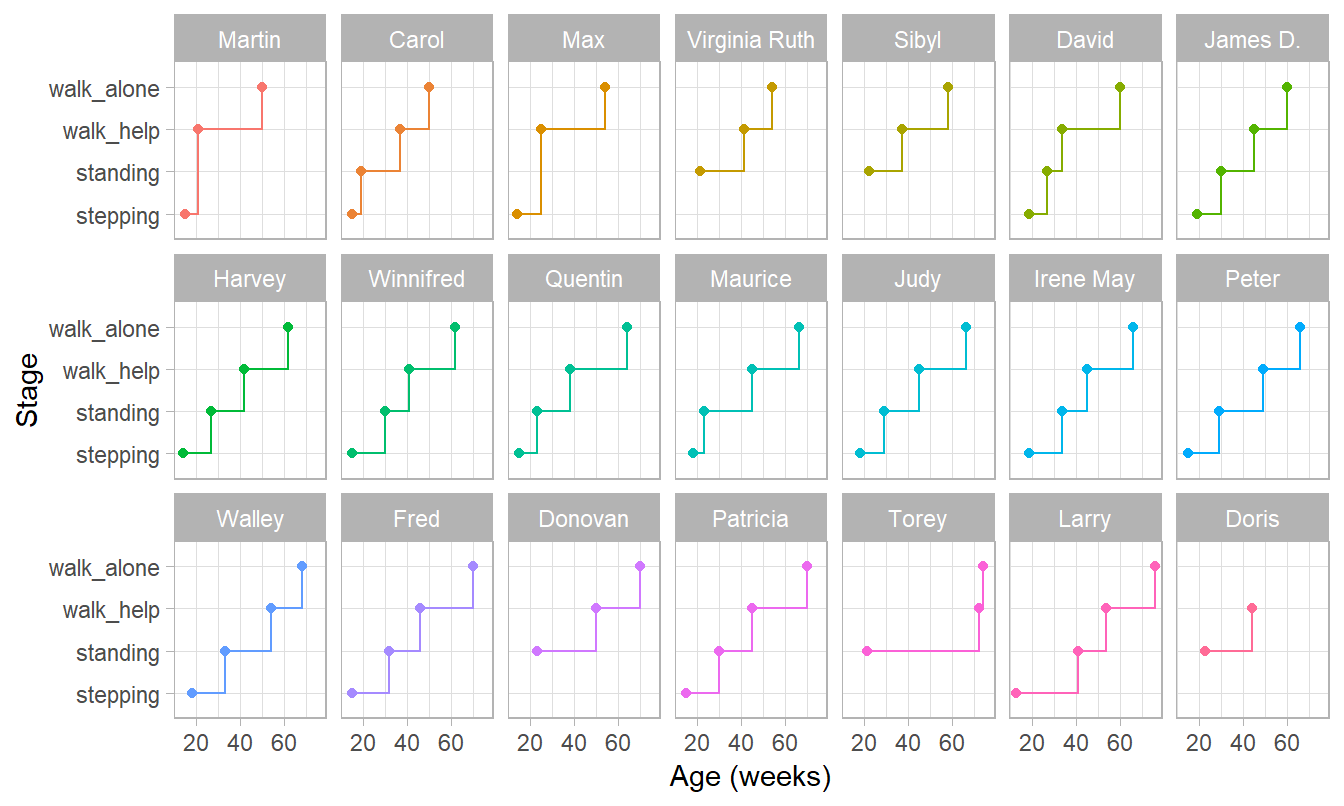
\includegraphics[width=1\linewidth]{dbook1_files/figure-latex/stepplot-1} 

}

\caption{Staircase plot indicating the age at which each baby achieves a new milestone of gross-motor functioning.}\label{fig:stepplot}
\end{figure}



Figure \ref{fig:stepplot} is a visual representation of the information in Table \ref{tab:shirley}. Each data point is the age of the first occurrence of the next stage. Before that age, we assume the baby is in the previous stage.

Figure \ref{fig:stepplot} makes it easy to spot the quick walkers (Martin, Carol) and slow walkers (Patricia, Torey, Larry). Furthermore, we may also locate children who remain a long time in a particular stage (Torey, Larry) or who jump over stages (Martin, Max).

For ease of plotting, the categories on the vertical axis are equally spaced. The height of the jump from one stage to the next has no sensible interpretation. We might be inclined to think that the vertical distance portrays to how difficult it is to achieve the next stage, but this is inaccurate. Instead, the ability needed to set the next step corresponds to the \emph{horizontal line length} between stages. For example, on average, the line for \texttt{stepping} is rather short in all plots, so going from \texttt{stepping} to \texttt{standing} is relatively easy.

Figure \ref{fig:stepplot} presents data from only those visits where a jump occurred. The number of house visits made during the ages of 0-2 years was far higher. \protect\hyperlink{ref-shirley1931}{Shirley} (\protect\hyperlink{ref-shirley1931}{1931}) collected data from 1370 visits, whereas Figure \ref{fig:stepplot} plot only the 76 occasions that showed a jump. Thus the data collection needs to be intense and costly to obtain individual curves. Fortunately, there are alternatives that are much more efficient.

\hypertarget{sec:questions}{%
\section{Typical questions asked in child development}\label{sec:questions}}

The emotional, social and physical development of the young child has a direct effect on the adult he or she will become. We may be interested in measuring child development for answering clinical, policy or public health questions.

\begin{verbatim}
Warning: Warning: fonts used in `flextable` are ignored because the `pdflatex`
engine is used and not `xelatex` or `lualatex`. You can avoid this warning
by using the `set_flextable_defaults(fonts_ignore=TRUE)` command or use a
compatible engine by defining `latex_engine: xelatex` in the YAML header of the
R Markdown document.
\end{verbatim}

\providecommand{\docline}[3]{\noalign{\global\setlength{\arrayrulewidth}{#1}}\arrayrulecolor[HTML]{#2}\cline{#3}}

\setlength{\tabcolsep}{2pt}

\renewcommand*{\arraystretch}{1.5}

\begin{longtable}[c]{cc}

\caption{Questions whose answers require quantitative measurements of child development.}\label{tab:questions}\\

\hhline{>{\arrayrulecolor[HTML]{666666}\global\arrayrulewidth=2pt}->{\arrayrulecolor[HTML]{666666}\global\arrayrulewidth=2pt}-}

\multicolumn{1}{!{\color[HTML]{000000}\vrule width 0pt}>{}l}{\fontsize{11}{11}\selectfont{\textcolor[HTML]{000000}{Level}}} & \multicolumn{1}{!{\color[HTML]{000000}\vrule width 0pt}>{}l!{\color[HTML]{000000}\vrule width 0pt}}{\fontsize{11}{11}\selectfont{\textcolor[HTML]{000000}{Question}}} \\

\noalign{\global\setlength{\arrayrulewidth}{2pt}}\arrayrulecolor[HTML]{666666}\cline{1-2}

\endfirsthead

\hhline{>{\arrayrulecolor[HTML]{666666}\global\arrayrulewidth=2pt}->{\arrayrulecolor[HTML]{666666}\global\arrayrulewidth=2pt}-}

\multicolumn{1}{!{\color[HTML]{000000}\vrule width 0pt}>{}l}{\fontsize{11}{11}\selectfont{\textcolor[HTML]{000000}{Level}}} & \multicolumn{1}{!{\color[HTML]{000000}\vrule width 0pt}>{}l!{\color[HTML]{000000}\vrule width 0pt}}{\fontsize{11}{11}\selectfont{\textcolor[HTML]{000000}{Question}}} \\

\noalign{\global\setlength{\arrayrulewidth}{2pt}}\arrayrulecolor[HTML]{666666}\cline{1-2}\endhead



\multicolumn{1}{!{\color[HTML]{000000}\vrule width 0pt}>{}l}{\fontsize{11}{11}\selectfont{\textcolor[HTML]{000000}{Individual}}} & \multicolumn{1}{!{\color[HTML]{000000}\vrule width 0pt}>{}l!{\color[HTML]{000000}\vrule width 0pt}}{\fontsize{11}{11}\selectfont{\textcolor[HTML]{000000}{What is the child's gain in development since the last visit?}}} \\





\multicolumn{1}{!{\color[HTML]{000000}\vrule width 0pt}>{}l}{\fontsize{11}{11}\selectfont{\textcolor[HTML]{000000}{Individual}}} & \multicolumn{1}{!{\color[HTML]{000000}\vrule width 0pt}>{}l!{\color[HTML]{000000}\vrule width 0pt}}{\fontsize{11}{11}\selectfont{\textcolor[HTML]{000000}{What is the difference in development between the child and peers of the same age?}}} \\





\multicolumn{1}{!{\color[HTML]{000000}\vrule width 0pt}>{}l}{\fontsize{11}{11}\selectfont{\textcolor[HTML]{000000}{Individual}}} & \multicolumn{1}{!{\color[HTML]{000000}\vrule width 0pt}>{}l!{\color[HTML]{000000}\vrule width 0pt}}{\fontsize{11}{11}\selectfont{\textcolor[HTML]{000000}{How does the child's development compare to a norm?}}} \\





\multicolumn{1}{!{\color[HTML]{000000}\vrule width 0pt}>{}l}{\fontsize{11}{11}\selectfont{\textcolor[HTML]{000000}{Group}}} & \multicolumn{1}{!{\color[HTML]{000000}\vrule width 0pt}>{}l!{\color[HTML]{000000}\vrule width 0pt}}{\fontsize{11}{11}\selectfont{\textcolor[HTML]{000000}{What is the effect of this intervention on child development?}}} \\





\multicolumn{1}{!{\color[HTML]{000000}\vrule width 0pt}>{}l}{\fontsize{11}{11}\selectfont{\textcolor[HTML]{000000}{Group}}} & \multicolumn{1}{!{\color[HTML]{000000}\vrule width 0pt}>{}l!{\color[HTML]{000000}\vrule width 0pt}}{\fontsize{11}{11}\selectfont{\textcolor[HTML]{000000}{What is the difference in child development between these two groups?}}} \\





\multicolumn{1}{!{\color[HTML]{000000}\vrule width 0pt}>{}l}{\fontsize{11}{11}\selectfont{\textcolor[HTML]{000000}{Population}}} & \multicolumn{1}{!{\color[HTML]{000000}\vrule width 0pt}>{}l!{\color[HTML]{000000}\vrule width 0pt}}{\fontsize{11}{11}\selectfont{\textcolor[HTML]{000000}{What is the change in average child development since the last measurement?}}} \\





\multicolumn{1}{!{\color[HTML]{000000}\vrule width 0pt}>{}l}{\fontsize{11}{11}\selectfont{\textcolor[HTML]{000000}{Population}}} & \multicolumn{1}{!{\color[HTML]{000000}\vrule width 0pt}>{}l!{\color[HTML]{000000}\vrule width 0pt}}{\fontsize{11}{11}\selectfont{\textcolor[HTML]{000000}{What was the effect of implementing this policy on child development?}}} \\





\multicolumn{1}{!{\color[HTML]{000000}\vrule width 0pt}>{}l}{\fontsize{11}{11}\selectfont{\textcolor[HTML]{000000}{Population}}} & \multicolumn{1}{!{\color[HTML]{000000}\vrule width 0pt}>{}l!{\color[HTML]{000000}\vrule width 0pt}}{\fontsize{11}{11}\selectfont{\textcolor[HTML]{000000}{How does this country compare to other countries in terms of child development?}}} \\

\noalign{\global\setlength{\arrayrulewidth}{2pt}}\arrayrulecolor[HTML]{666666}\cline{1-2}

\end{longtable}

Table \ref{tab:questions} lists typical questions whose answers require measuring child development. Note that all questions compare the amount of child development between groups or time points. A few questions compare development for the same child, group or population at different ages. Others compare development at the same age across different children, groups or populations.

\newpage

\hypertarget{ch:threeways}{%
\chapter{Quantifying child development}\label{ch:threeways}}

This section discusses four principles to quantify child development:

\begin{itemize}
\tightlist
\item
  Age-based measurement (\ref{sec:agebased})
\item
  Probability-based measurement (\ref{sec:probbased})
\item
  Score-based measurement (\ref{sec:scorebased})
\item
  Unit-based measurement (\ref{sec:unitbased})
\end{itemize}

\hypertarget{sec:agebased}{%
\section{Age-based measurement of development}\label{sec:agebased}}

\hypertarget{motivation-for-age-based-measurement}{%
\subsection{Motivation for age-based measurement}\label{motivation-for-age-based-measurement}}

Milestones form the based building blocks for instruments to measure child development. Methods to quantify growth using separate milestones relate the milestone behaviour to the child's age. \protect\hyperlink{ref-gesell1943}{Gesell} (\protect\hyperlink{ref-gesell1943}{1943}) (p.~89) formulated this goal as follows:

\begin{quote}
We think of behaviour in terms of age, and we think of age in terms of behaviour. For any selected age it is possible to sketch a portrait which delineates the behaviour characteristics typical of the age.
\end{quote}

There is an extensive literature that quantifies development in terms of the ages at which the child is expected to show a specific behaviour. The oldest methods for quantifying child development calculate an \emph{age equivalent} for achieving a milestone, and compare the child's age to this age equivalent.

\hypertarget{sec:ageequivalent}{%
\subsection{Age equivalent and developmental age}\label{sec:ageequivalent}}

\begin{figure}

{\centering 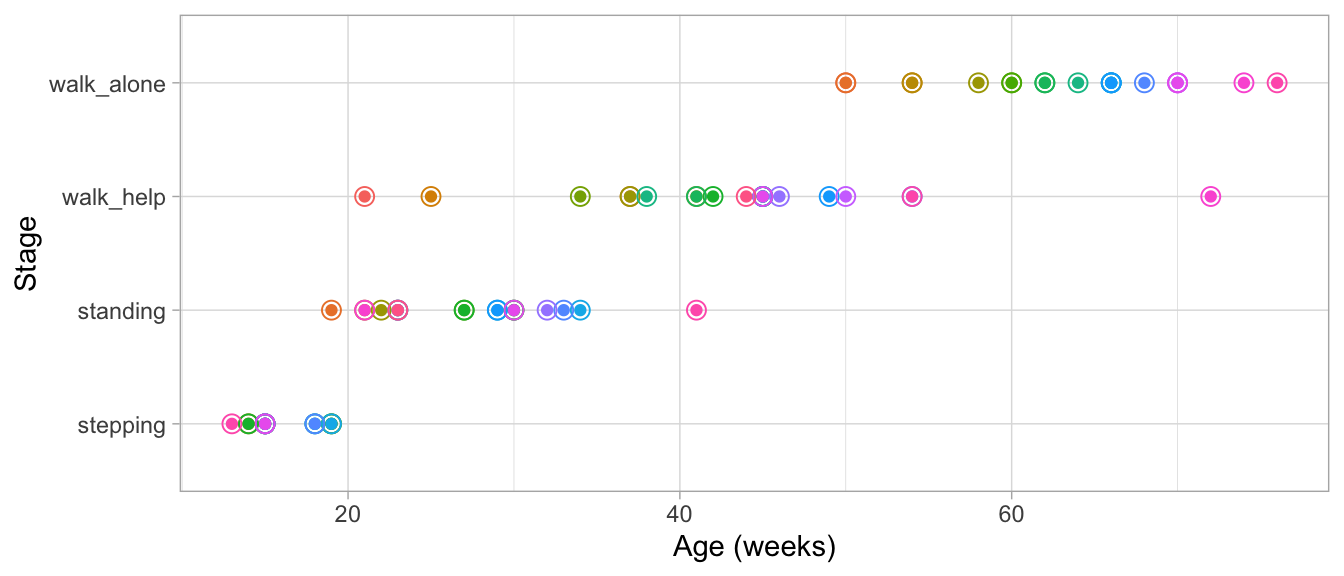
\includegraphics[width=1\linewidth]{dbook1_files/figure-latex/milestonebased-1} 

}

\caption{Ages at which 21 children achieve four motor development milestones.}\label{fig:milestonebased}
\end{figure}



Figure \ref{fig:milestonebased} graphs the ages at which each of the 21 children enter a given stage in Shirley's motor data of Table \ref{tab:shirley}. Since \texttt{standing} follows \texttt{stepping}, children who can stand are older than the children who are stepping. Hence the ages for standing are located more to the right.

Since age and development are so intimately related, we can express the \emph{difficulty} of a milestone as the \emph{mean age} at which children achieve it. For example, \protect\hyperlink{ref-stott1967}{Stott} (\protect\hyperlink{ref-stott1967}{1967}) (p.~25) defines the \emph{age equivalent} and its use for measurement, as follows:

\begin{quote}
The age equivalent of a particular stage is simply the average age at which children reach that particular stage.
\end{quote}

\begin{figure}

{\centering 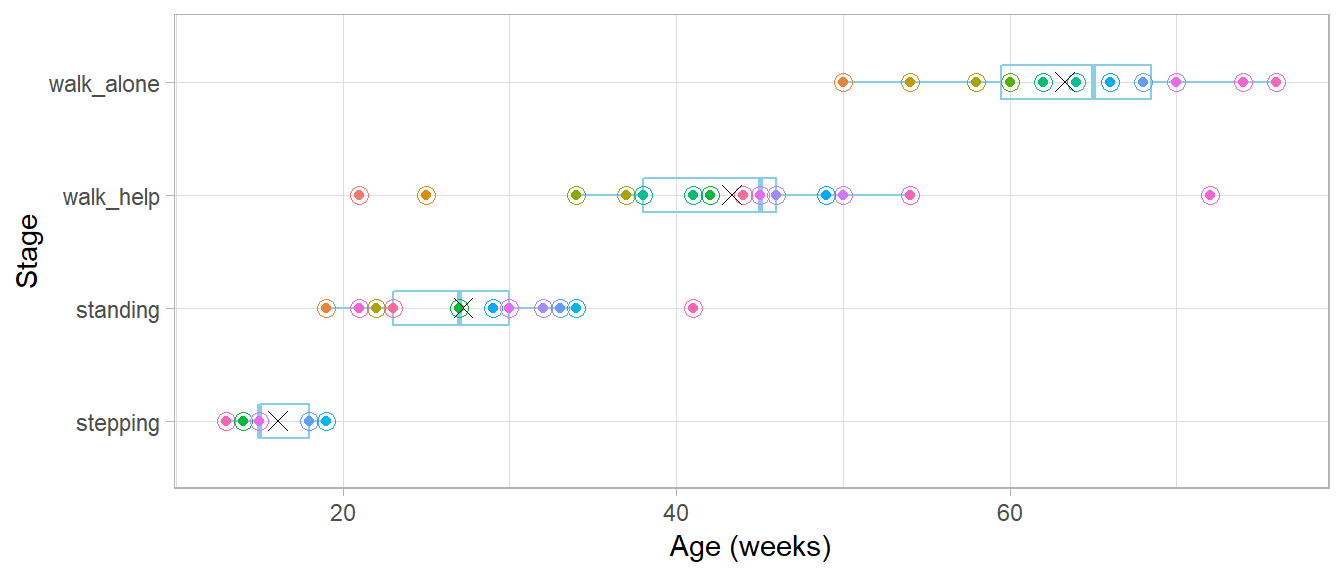
\includegraphics[width=1\linewidth]{dbook1_files/figure-latex/agebox-1} 

}

\caption{Mean (symbol \texttt{x}) and spread of the ages at which 21 children achieve four motor development milestones.}\label{fig:agebox}
\end{figure}



Figure \ref{fig:agebox} adds the mean age and the boxplot at which the children enter the four stages. The difficulty of these milestones can thus be expressed as age equivalents: 16.1 weeks for \texttt{stepping}, 27.2 weeks for \texttt{standing}, 43.3 weeks for \texttt{walking\ with\ help} and 63.3 weeks for \texttt{walking\ alone}.

Thus, a child that is stepping beyond the age of 16.1 weeks is considered later than average, whereas a child already stepping before 27.2 weeks earlier than average. We may also calculate age delta as the difference between the child's age and the norm age, and express it as ``two weeks late'' or ``three weeks ahead.'' Summarizing age delta's over different milestones has led to concepts like \emph{developmental age} as a measure of a child's development.

\hypertarget{limitations-of-age-based-measurement}{%
\subsection{Limitations of age-based measurement}\label{limitations-of-age-based-measurement}}

Age-based measurement is easy to understand, and widely used in the popular press, but not without pitfalls:

\begin{enumerate}
\def\labelenumi{\arabic{enumi}.}
\tightlist
\item
  Age-based measurement requires us to know the ages at which the child entered a new stage. The mean age can be a biased estimate of item difficulty if visits are widely apart, irregular or missing.
\item
  Age-based measurement can inform us whether a child is achieving a given milestone early of late. However, it does not tell us what behaviours are characteristic for children of a given age.
\item
  Age-based measurement cannot exist without an age norm. When there are no norms, we cannot quantify development.
\item
  Age-based measurement works only at the item level. Although we may average age delta's over milestones, the choice of milestones is arbitrary.
\end{enumerate}

\hypertarget{sec:probbased}{%
\section{Probability-based measurement}\label{sec:probbased}}

An alternative is to calculate the \emph{probability} of achieving a milestone at a given age and compare the child's response to that probability.

The passing probability is an interpretable and relevant measure. An operational advantage of the approach is that the necessary calculations place fewer demands on the available data and can be done even for cross-sectional studies.

\hypertarget{example-of-probability-based-measurement}{%
\subsection{Example of probability-based measurement}\label{example-of-probability-based-measurement}}

\begin{figure}

{\centering 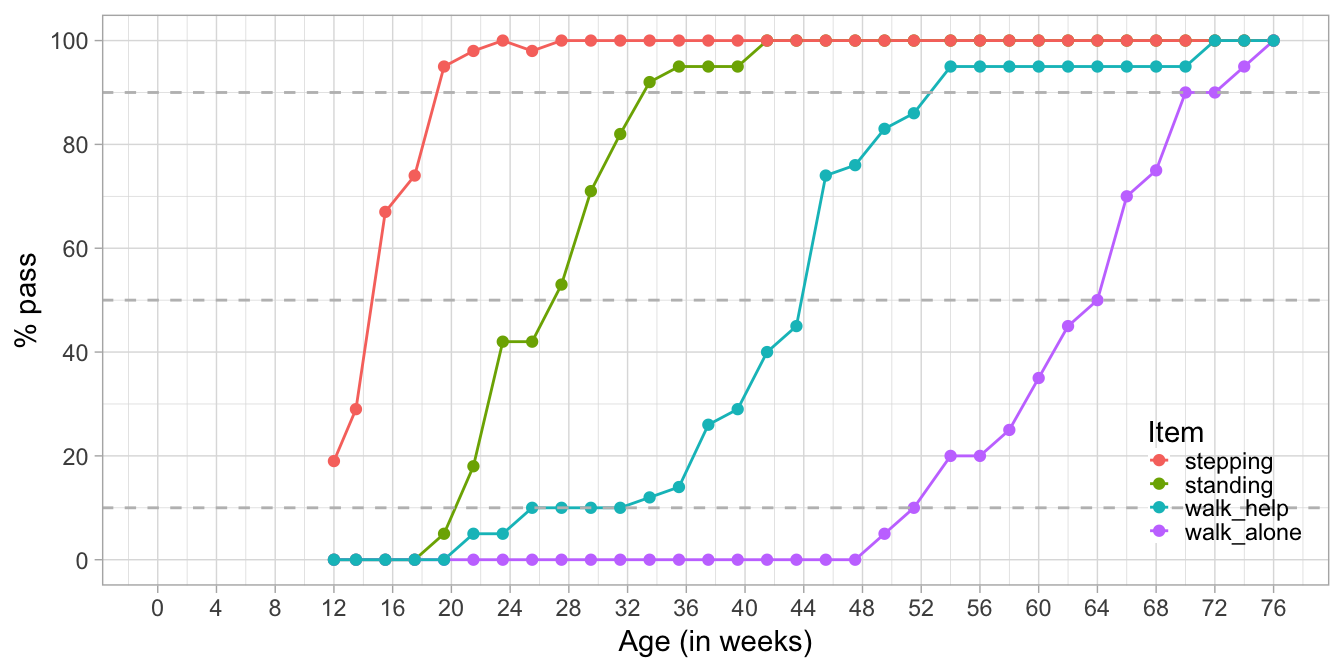
\includegraphics[width=1\linewidth]{dbook1_files/figure-latex/shirleypa-1} 

}

\caption{Probability of achieving four motor milestones against age.}\label{fig:shirleypa}
\end{figure}



Figure \ref{fig:shirleypa} plots the percentage of children achieving each of Shirley's motor stages against age. There are four cumulative curves, one for each milestone, that indicate the percentage of children that pass.

In analogy to the age equivalent introduced in Section \ref{sec:ageequivalent} we can define the \emph{difficulty} of the milestone as the age at which 50 per cent of the children pass. In the Figure we see that the levels of difficulty are approximately 14.2 weeks (\texttt{stepping}), 27.0 weeks (\texttt{standing}), 43.8 weeks (\texttt{walking\ with\ help}) and 64.0 weeks (\texttt{walking\ alone}). Also, we may easily find the ages at which 10 per cent or 90 per cent of the children pass each milestone.

Observe there is a gradual decline in the steepness as we move from \texttt{stepping} to \texttt{walk\_alone}. For example, we need an age interval of 13 weeks (33 - 20) to go from 10 to 90 per cent in \texttt{standing}, but need 19 weeks (71 - 52) to go from 10 to 90 per cent in \texttt{walking\ alone}. Thus, one step on the age axis corresponds to different increments in probability. The flattening pattern is typical for child development and represents evidence that evolution is faster at earlier ages.

\hypertarget{limitations-of-probability-based-measurement}{%
\subsection{Limitations of probability-based measurement}\label{limitations-of-probability-based-measurement}}

Probability-based measurement is a popular way to create instruments for screening on developmental delay. For example, each milestone in the Denver II (\protect\hyperlink{ref-frankenburg1992}{Frankenburg et al. 1992}) has markers for the 25th, 50th, 75th and 90th age percentile.

\begin{enumerate}
\def\labelenumi{\arabic{enumi}.}
\tightlist
\item
  The same age step corresponds to different probabilities.
\item
  The measurement cannot exist without some norm population. When norms differ, we cannot compare the measurements.
\item
  Interpretation is at the milestone level, sometimes supplemented by procedures for counting the number of delays. No aggregate takes all responses into account.
\end{enumerate}

\hypertarget{sec:scorebased}{%
\section{Score-based measurement of development}\label{sec:scorebased}}

\hypertarget{sec:motivscorebased}{%
\subsection{Motivation for score-based measurement}\label{sec:motivscorebased}}

Score-based measurement takes the responses on multiple milestones and counts the total number of items passed as a measure of development. This approach takes all answers into account, hence leading to a more stable result.

One may order milestones in difficulty, and skip those that are too easy, and stop administration for those that are too difficult. In such cases, we cannot merely interpret the sum score of a measure of development. Instead, we need to correct for the subset of administered milestones. The usual working assumption is that the child would have passed all easier milestones and failed on all more difficult ones. We may repeat this procedure for different domains, e.g.~motor, cognitive, and so on.

\hypertarget{example-of-score-based-measurement}{%
\subsection{Example of score-based measurement}\label{example-of-score-based-measurement}}

Figure \ref{fig:scoreplot} is a gross-motor score calculated as the number of milestones passed. It varies from 0 to 3.

\begin{figure}

{\centering 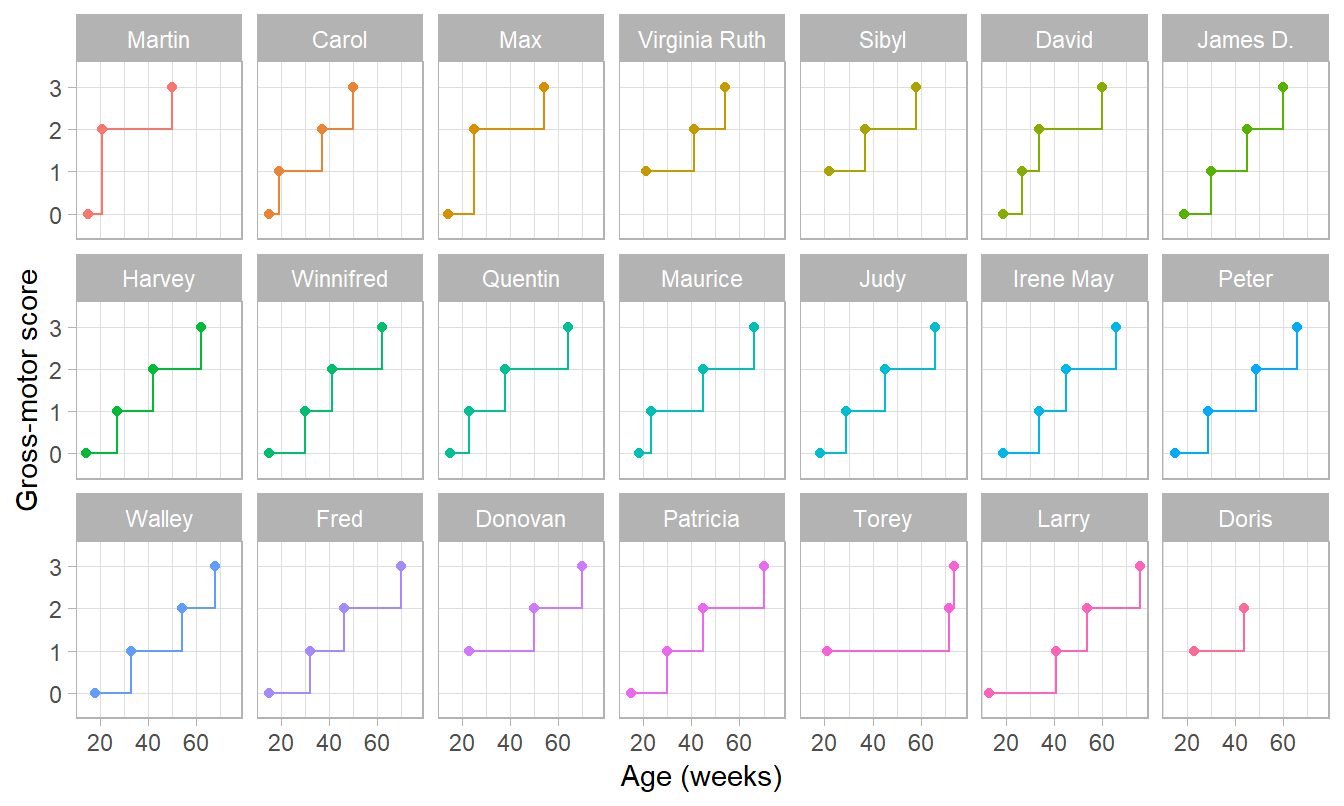
\includegraphics[width=1\linewidth]{dbook1_files/figure-latex/scoreplot-1} 

}

\caption{Same data as in Figure \ref{fig:stepplot}, but now with the vertical axis representing gross-motor score.}\label{fig:scoreplot}
\end{figure}



The plot suggests that the difference in development between scores 0 and 1 is the same as the difference between, say, scores 2 and 3. \emph{This is not correct}. For example, suppose that we express the difficulty of the milestone as an age-equivalent. From section \ref{sec:ageequivalent} we see that the difference between stepping and standing is 27.2 - 16.1 = 11.1 weeks, whereas the difference between walking alone and walking with help is 63.3 - 43.3 = 20 weeks. Thus, according to age equivalents scores 0 and 1 should be closer to each other, and ratings 2 and 3 should be drawn more apart.

\hypertarget{limitations-of-score-based-measurement}{%
\subsection{Limitations of score-based measurement}\label{limitations-of-score-based-measurement}}

Score-based measurement is today's dominant approach, but is not without conceptual and logistical issues.

\begin{enumerate}
\def\labelenumi{\arabic{enumi}.}
\tightlist
\item
  The total score depends not only on the actual developmental status of the child, but also on the set of milestones administered. If a milestone is skipped or added, the sum score cannot be interpreted anymore as a measure of developmental status. It might be possible to correct for starting and stopping rules under the assumptions described in Section \ref{sec:motivscorebased}, but such will be involved if intermediate milestones are missing.
\item
  It is not possible to compare the scores made by different instruments. Some instruments allow conversion to age-conditional scores. However, the sample used to derive such transformations pertain to that tool and does not generalise to others.
\item
  Domains are hard to separate. For example, some cognitive milestones tap into fine motor capabilities, and vice versa. There are different ways to define domains, so domain interpretation varies by instrument.
\item
  Administration of a full test may take substantial time. The materials are often proprietary and costly.
\end{enumerate}

\hypertarget{sec:unitbased}{%
\section{Unit-based measurement of development}\label{sec:unitbased}}

\hypertarget{sec:motivationunit}{%
\subsection{Motivation for unit-based measurement}\label{sec:motivationunit}}

Unit-based measurement starts by defining ideal properties and derives a procedure to aggregate the responses on milestones into an overall score that will meet this ideal.

Section \ref{sec:questions} highlighted questions for individuals, groups and populations. There are three questions:

\begin{itemize}
\tightlist
\item
  What is the difference in development over time for the same child, group or community?
\item
  What is the difference in development between different children, groups or populations of the same age?
\item
  How does child development compare to a norm?
\end{itemize}

In the ideal situation, we would like to have a continuous (latent) variable \(D\) (for development) that measures child development. The scale should allow us to quantify \emph{ability} of persons, groups or populations from low to high. It should have a \emph{constant unit} so that a given difference in ability refers to the same quantity across the entire scale. We find the same property in height, where a distance of 10 cm represents the same amount for molecules, people or galaxies. When are these conditions are met, we say that we measure on an \emph{interval scale}.

If we succeed in creating an interval scale for child development, an enormous arsenal of techniques developed for quantitative variables opens up to measure, track and analyze child development. We may then evaluate the status of a child in terms of \(D\) points gained, create age-dependent diagrams (just like growth charts for height and weight), devise age-conditional measures for child development, and intelligent adaptive testing schemes. Promising studies on Dutch data \protect\hyperlink{ref-vanbuuren2014}{van Buuren} (\protect\hyperlink{ref-vanbuuren2014}{2014}) suggest that such benefits are well within reach.

\hypertarget{sec:unitbasedexample}{%
\subsection{Example of unit-based measurement}\label{sec:unitbasedexample}}

\begin{figure}

{\centering 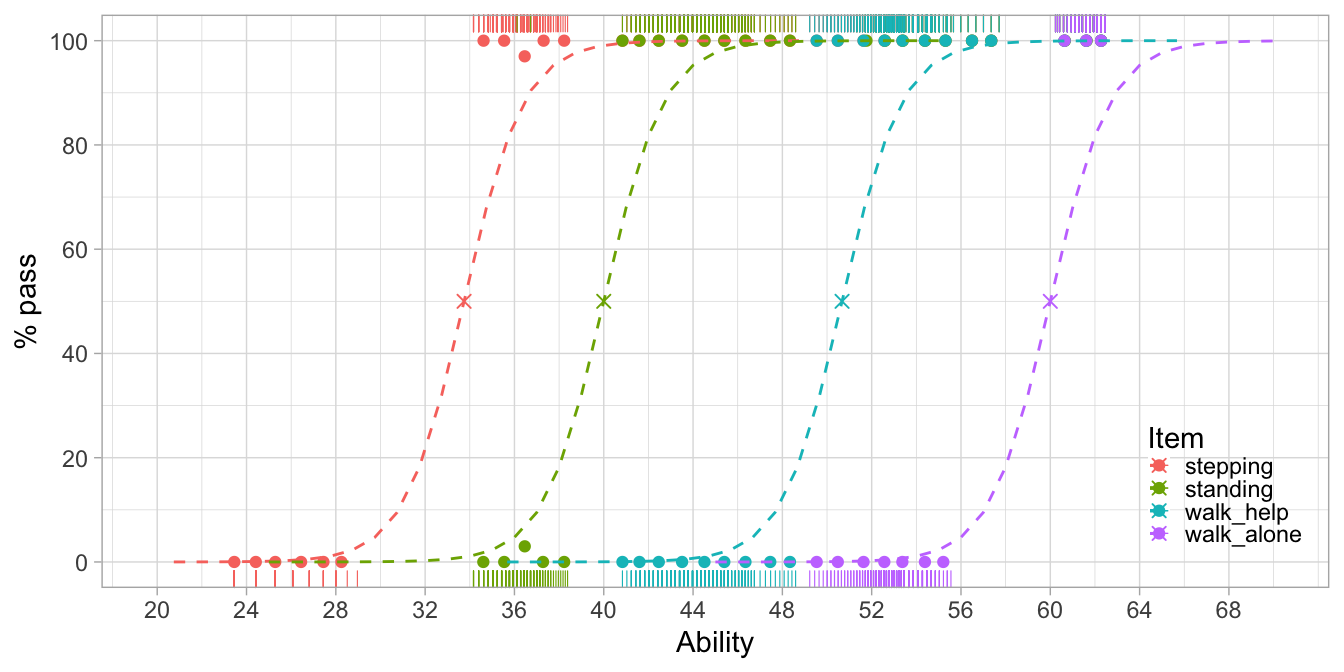
\includegraphics[width=1\linewidth]{dbook1_files/figure-latex/shirleypd-1} 

}

\caption{Modeled probability of achieving four motor milestones against the D-score.}\label{fig:shirleypd}
\end{figure}



Figure \ref{fig:shirleypd} is similar to Figure \ref{fig:shirleypa}, but with \texttt{Age} replaced by \texttt{Ability}. Also, modelled curves have replaced empirical ones, but this is not essential.

We estimated the ability values on the horizontal axis from the data. The values correspond to the amount of development of each visit. Likewise, we calculated the logistic curves from the data. These reflect the probability of passing each milestone \emph{at a given level of ability}.

Figure \ref{fig:shirleypd} shows that the probability of passing a milestone increases with ability. Items are sorted according to difficulty from left to right. Milestone \texttt{stepping} is the easiest and \texttt{walk\_alone} is the most difficult. The point at which a logistic curve crosses the 50 per cent line (marked by a cross) is the \emph{difficulty of the milestone}.

The increase in ability that is needed to go from 10 to 90 per cent is about five units here. Since all curves are parallel, the interval is constant for all scale locations. Thus, the scale is an \emph{interval scale} with a \emph{constant unit of measurement}, the type of measurement needed for answering the basic questions identified in Section \ref{sec:motivationunit}.

\hypertarget{limitations-of-unit-based-measurement}{%
\subsection{Limitations of unit-based measurement}\label{limitations-of-unit-based-measurement}}

While unit-based measurement has many advantages, it cannot perform miracles.

\begin{enumerate}
\def\labelenumi{\arabic{enumi}.}
\tightlist
\item
  An important assumption is that the milestones ``measure the same thing,'' or put differently, are manifestations of a continuous latent variable that can be measured by empirical observations. Unit-based measurement won't work if there is no sensible latent scale.
\item
  The portrayed advantages hold only if the discrepancies between the data and the model are relatively small. Since the simplest and most powerful measurement models are strict, it is essential to obtain a good fit between the data and the model.
\item
  The construction of unit-based measurement requires psychometric expertise, specialized computer software and considerable sample sizes.
\end{enumerate}

\hypertarget{sec:whatismeasurement}{%
\section{A unified framework}\label{sec:whatismeasurement}}

This section brings together the four approaches outlined in this section into a unified framework.

\begin{figure}

{\centering 
\includegraphics[width=1\linewidth]{fig/lineplot} 

}

\caption{Placing milestones and children onto the same line reveals their positions.}\label{fig:lineplot}
\end{figure}



Figure \ref{fig:lineplot} shows the imaginary positions on a gross-motor continuum of three babies from Figure \ref{fig:shirleyplot} at the age of 30 weeks. Both milestones and children are ordered along the same continuum. Thus, standing is more difficult than stepping, and at week 30, Doris is ahead of Walley in terms of motor development.

More generally, measurement is the process of locating milestones and children on a line. This line represents a \emph{latent variable}, a continuous construct that defines the different poles of the concept that we want to measure. A latent variable ranges from low to high.

The first part of measurement is to determine the location of the milestones on the latent variable. In many cases, the instrument maker has already done that. For example, each length marker on a ruler corresponds to a milestone for measuring length. The manufacturer of the ruler has already placed the marks at the appropriate places on the tool, and we take for granted that each marker has been calibrated correctly.

A milestone for child development is similar to a length marker, but

\begin{itemize}
\tightlist
\item
  we may not know how much development the milestone measures, so its location on the line is unknown, or uncertain;
\item
  we may not know whether the milestone measures child development at all so that it may have no location on the line.
\end{itemize}

The second part of measurement is to find the location of each child on the line. For child height, this is easy: We place the horizontal headpiece on top of the child's head and read off the closest height marker. Since we lack a physical ruler for development, we must deduce the child's location on the line from the responses on a series of well-chosen milestones.

By definition, we cannot observe the values of a latent variable directly. However, we may be able to measure variables (milestones) that are related to the latent variable. For example, we may have scores on tasks like \emph{standing} or \emph{walking with help}.

The \emph{measurement model} specifies the relations between the actual measurements and the latent variable. Under a given measurement model, we may estimate the locations of milestones and children on the line. Section \ref{sec:measurementmodel} discusses measurement models in more detail.

\hypertarget{sec:whyunit}{%
\section{Why unit-based measurement}\label{sec:whyunit}}

\begin{verbatim}
Warning: Warning: fonts used in `flextable` are ignored because the `pdflatex`
engine is used and not `xelatex` or `lualatex`. You can avoid this warning
by using the `set_flextable_defaults(fonts_ignore=TRUE)` command or use a
compatible engine by defining `latex_engine: xelatex` in the YAML header of the
R Markdown document.
\end{verbatim}

\providecommand{\docline}[3]{\noalign{\global\setlength{\arrayrulewidth}{#1}}\arrayrulecolor[HTML]{#2}\cline{#3}}

\setlength{\tabcolsep}{2pt}

\renewcommand*{\arraystretch}{1.5}

\begin{longtable}[c]{ccccc}

\caption{Evaluation of four measurement approaches on seven criteria.}\label{tab:measurement}\\

\hhline{>{\arrayrulecolor[HTML]{666666}\global\arrayrulewidth=2pt}->{\arrayrulecolor[HTML]{666666}\global\arrayrulewidth=2pt}->{\arrayrulecolor[HTML]{666666}\global\arrayrulewidth=2pt}->{\arrayrulecolor[HTML]{666666}\global\arrayrulewidth=2pt}->{\arrayrulecolor[HTML]{666666}\global\arrayrulewidth=2pt}-}

\multicolumn{1}{!{\color[HTML]{000000}\vrule width 0pt}>{}l}{\fontsize{11}{11}\selectfont{\textcolor[HTML]{000000}{Criterion}}} & \multicolumn{1}{!{\color[HTML]{000000}\vrule width 0pt}>{}l}{\fontsize{11}{11}\selectfont{\textcolor[HTML]{000000}{Age}}} & \multicolumn{1}{!{\color[HTML]{000000}\vrule width 0pt}>{}l}{\fontsize{11}{11}\selectfont{\textcolor[HTML]{000000}{Probability}}} & \multicolumn{1}{!{\color[HTML]{000000}\vrule width 0pt}>{}l}{\fontsize{11}{11}\selectfont{\textcolor[HTML]{000000}{Score}}} & \multicolumn{1}{!{\color[HTML]{000000}\vrule width 0pt}>{}l!{\color[HTML]{000000}\vrule width 0pt}}{\fontsize{11}{11}\selectfont{\textcolor[HTML]{000000}{Unit}}} \\

\noalign{\global\setlength{\arrayrulewidth}{2pt}}\arrayrulecolor[HTML]{666666}\cline{1-5}

\endfirsthead

\hhline{>{\arrayrulecolor[HTML]{666666}\global\arrayrulewidth=2pt}->{\arrayrulecolor[HTML]{666666}\global\arrayrulewidth=2pt}->{\arrayrulecolor[HTML]{666666}\global\arrayrulewidth=2pt}->{\arrayrulecolor[HTML]{666666}\global\arrayrulewidth=2pt}->{\arrayrulecolor[HTML]{666666}\global\arrayrulewidth=2pt}-}

\multicolumn{1}{!{\color[HTML]{000000}\vrule width 0pt}>{}l}{\fontsize{11}{11}\selectfont{\textcolor[HTML]{000000}{Criterion}}} & \multicolumn{1}{!{\color[HTML]{000000}\vrule width 0pt}>{}l}{\fontsize{11}{11}\selectfont{\textcolor[HTML]{000000}{Age}}} & \multicolumn{1}{!{\color[HTML]{000000}\vrule width 0pt}>{}l}{\fontsize{11}{11}\selectfont{\textcolor[HTML]{000000}{Probability}}} & \multicolumn{1}{!{\color[HTML]{000000}\vrule width 0pt}>{}l}{\fontsize{11}{11}\selectfont{\textcolor[HTML]{000000}{Score}}} & \multicolumn{1}{!{\color[HTML]{000000}\vrule width 0pt}>{}l!{\color[HTML]{000000}\vrule width 0pt}}{\fontsize{11}{11}\selectfont{\textcolor[HTML]{000000}{Unit}}} \\

\noalign{\global\setlength{\arrayrulewidth}{2pt}}\arrayrulecolor[HTML]{666666}\cline{1-5}\endhead



\multicolumn{1}{!{\color[HTML]{000000}\vrule width 0pt}>{}l}{\fontsize{11}{11}\selectfont{\textcolor[HTML]{000000}{Independent of age norm}}} & \multicolumn{1}{!{\color[HTML]{000000}\vrule width 0pt}>{}l}{\fontsize{11}{11}\selectfont{\textcolor[HTML]{000000}{No}}} & \multicolumn{1}{!{\color[HTML]{000000}\vrule width 0pt}>{}l}{\fontsize{11}{11}\selectfont{\textcolor[HTML]{000000}{No}}} & \multicolumn{1}{!{\color[HTML]{000000}\vrule width 0pt}>{}l}{\fontsize{11}{11}\selectfont{\textcolor[HTML]{000000}{Yes}}} & \multicolumn{1}{!{\color[HTML]{000000}\vrule width 0pt}>{}l!{\color[HTML]{000000}\vrule width 0pt}}{\fontsize{11}{11}\selectfont{\textcolor[HTML]{000000}{Yes}}} \\





\multicolumn{1}{!{\color[HTML]{000000}\vrule width 0pt}>{}l}{\fontsize{11}{11}\selectfont{\textcolor[HTML]{000000}{Supports multiple milestones}}} & \multicolumn{1}{!{\color[HTML]{000000}\vrule width 0pt}>{}l}{\fontsize{11}{11}\selectfont{\textcolor[HTML]{000000}{No}}} & \multicolumn{1}{!{\color[HTML]{000000}\vrule width 0pt}>{}l}{\fontsize{11}{11}\selectfont{\textcolor[HTML]{000000}{No}}} & \multicolumn{1}{!{\color[HTML]{000000}\vrule width 0pt}>{}l}{\fontsize{11}{11}\selectfont{\textcolor[HTML]{000000}{Yes}}} & \multicolumn{1}{!{\color[HTML]{000000}\vrule width 0pt}>{}l!{\color[HTML]{000000}\vrule width 0pt}}{\fontsize{11}{11}\selectfont{\textcolor[HTML]{000000}{Yes}}} \\





\multicolumn{1}{!{\color[HTML]{000000}\vrule width 0pt}>{}l}{\fontsize{11}{11}\selectfont{\textcolor[HTML]{000000}{Latent variable}}} & \multicolumn{1}{!{\color[HTML]{000000}\vrule width 0pt}>{}l}{\fontsize{11}{11}\selectfont{\textcolor[HTML]{000000}{No}}} & \multicolumn{1}{!{\color[HTML]{000000}\vrule width 0pt}>{}l}{\fontsize{11}{11}\selectfont{\textcolor[HTML]{000000}{No}}} & \multicolumn{1}{!{\color[HTML]{000000}\vrule width 0pt}>{}l}{\fontsize{11}{11}\selectfont{\textcolor[HTML]{000000}{Yes}}} & \multicolumn{1}{!{\color[HTML]{000000}\vrule width 0pt}>{}l!{\color[HTML]{000000}\vrule width 0pt}}{\fontsize{11}{11}\selectfont{\textcolor[HTML]{000000}{Yes}}} \\





\multicolumn{1}{!{\color[HTML]{000000}\vrule width 0pt}>{}l}{\fontsize{11}{11}\selectfont{\textcolor[HTML]{000000}{Robust to milestone skipping}}} & \multicolumn{1}{!{\color[HTML]{000000}\vrule width 0pt}>{}l}{\fontsize{11}{11}\selectfont{\textcolor[HTML]{000000}{Yes}}} & \multicolumn{1}{!{\color[HTML]{000000}\vrule width 0pt}>{}l}{\fontsize{11}{11}\selectfont{\textcolor[HTML]{000000}{Yes}}} & \multicolumn{1}{!{\color[HTML]{000000}\vrule width 0pt}>{}l}{\fontsize{11}{11}\selectfont{\textcolor[HTML]{000000}{No}}} & \multicolumn{1}{!{\color[HTML]{000000}\vrule width 0pt}>{}l!{\color[HTML]{000000}\vrule width 0pt}}{\fontsize{11}{11}\selectfont{\textcolor[HTML]{000000}{Yes}}} \\





\multicolumn{1}{!{\color[HTML]{000000}\vrule width 0pt}>{}l}{\fontsize{11}{11}\selectfont{\textcolor[HTML]{000000}{Comparable scores}}} & \multicolumn{1}{!{\color[HTML]{000000}\vrule width 0pt}>{}l}{\fontsize{11}{11}\selectfont{\textcolor[HTML]{000000}{Yes}}} & \multicolumn{1}{!{\color[HTML]{000000}\vrule width 0pt}>{}l}{\fontsize{11}{11}\selectfont{\textcolor[HTML]{000000}{Yes}}} & \multicolumn{1}{!{\color[HTML]{000000}\vrule width 0pt}>{}l}{\fontsize{11}{11}\selectfont{\textcolor[HTML]{000000}{No}}} & \multicolumn{1}{!{\color[HTML]{000000}\vrule width 0pt}>{}l!{\color[HTML]{000000}\vrule width 0pt}}{\fontsize{11}{11}\selectfont{\textcolor[HTML]{000000}{Yes}}} \\





\multicolumn{1}{!{\color[HTML]{000000}\vrule width 0pt}>{}l}{\fontsize{11}{11}\selectfont{\textcolor[HTML]{000000}{Probability model}}} & \multicolumn{1}{!{\color[HTML]{000000}\vrule width 0pt}>{}l}{\fontsize{11}{11}\selectfont{\textcolor[HTML]{000000}{No}}} & \multicolumn{1}{!{\color[HTML]{000000}\vrule width 0pt}>{}l}{\fontsize{11}{11}\selectfont{\textcolor[HTML]{000000}{Yes}}} & \multicolumn{1}{!{\color[HTML]{000000}\vrule width 0pt}>{}l}{\fontsize{11}{11}\selectfont{\textcolor[HTML]{000000}{No}}} & \multicolumn{1}{!{\color[HTML]{000000}\vrule width 0pt}>{}l!{\color[HTML]{000000}\vrule width 0pt}}{\fontsize{11}{11}\selectfont{\textcolor[HTML]{000000}{Yes}}} \\





\multicolumn{1}{!{\color[HTML]{000000}\vrule width 0pt}>{}l}{\fontsize{11}{11}\selectfont{\textcolor[HTML]{000000}{Defines measurement unit}}} & \multicolumn{1}{!{\color[HTML]{000000}\vrule width 0pt}>{}l}{\fontsize{11}{11}\selectfont{\textcolor[HTML]{000000}{No}}} & \multicolumn{1}{!{\color[HTML]{000000}\vrule width 0pt}>{}l}{\fontsize{11}{11}\selectfont{\textcolor[HTML]{000000}{No}}} & \multicolumn{1}{!{\color[HTML]{000000}\vrule width 0pt}>{}l}{\fontsize{11}{11}\selectfont{\textcolor[HTML]{000000}{No}}} & \multicolumn{1}{!{\color[HTML]{000000}\vrule width 0pt}>{}l!{\color[HTML]{000000}\vrule width 0pt}}{\fontsize{11}{11}\selectfont{\textcolor[HTML]{000000}{Yes}}} \\

\noalign{\global\setlength{\arrayrulewidth}{2pt}}\arrayrulecolor[HTML]{666666}\cline{1-5}

\end{longtable}

This section distinguished four approaches to measure child development: \emph{age-based}, \emph{probability-based}, \emph{score-based} and \emph{unit-based} measurement. Table \ref{tab:measurement} summarizes how the approaches evaluate on nine criteria.

\emph{Age-based measurement} expresses development in age equivalents, whose precise definition depends on the reference population. Age-based measurement does not support multiple milestones and does not use the concept of a latent variable.

\emph{Probability-based measurement} expresses development as age percentiles for a reference population. It is useful for individual milestones but does not support multiple items or a latent variable interpretation.

\emph{Score-based measurement} quantifies development by summing the number of passes. Different instruments make different selections of milestones, so the scores taken are unique to the tool. Thus comparing the measurement obtained by different devices is difficult. Skipping or adding items require corrections.

\emph{Unit-based measurement} defines a unit by a theoretical model. When the data fit the model, we are able to construct instruments that produce values in a standard metric.

\newpage

\hypertarget{ch:newmodel}{%
\chapter{The D-score}\label{ch:newmodel}}

Section \ref{ch:history} provided historical background on the nature of child development. Section \ref{ch:threeways} discussed three general quantification approaches. This section explains how to apply the unit-based approach to arrive at the D-score scale. The text illustrates the process with real data.

\begin{itemize}
\tightlist
\item
  Dutch Development Instrument (DDI) (\ref{sec:ddi})
\item
  Milestone passing by age and by D-score (\ref{sec:probage}, \ref{sec:probd})
\item
  How do age and D-score relate? (\ref{sec:aged})
\item
  Role of the measurement model (\ref{sec:measurementmodel})
\item
  Item and person response functions (\ref{sec:itemresponsefunctions})
\item
  Engelhard invariance criteria (\ref{sec:engelhard})
\item
  Why the Rasch model? (\ref{sec:whyrasch})
\end{itemize}

\hypertarget{sec:ddi}{%
\section{The Dutch Development Instrument (DDI)}\label{sec:ddi}}

\hypertarget{setting}{%
\subsection{Setting}\label{setting}}

The Dutch Youth Health Care (YHC) routinely monitors the development of almost all children living in The Netherlands. During the first four years, there are 13 scheduled visits. During these visits, the YHC professionals evaluate the growth and development of the child.

The \emph{Dutch Development Instrument} (DDI; in Dutch: \emph{Van Wiechenschema}) is the standard instrument used to measure development during the ages 0-4 years. The DDI consists of \href{https://www.ncj.nl/van-wiechen/kenmerken/}{75 milestones}. The instrument assesses three developmental domains:

\begin{enumerate}
\def\labelenumi{\arabic{enumi}.}
\tightlist
\item
  Fine motor, adaptation, personality and social behaviour;
\item
  Communication;
\item
  Gross motor.
\end{enumerate}

The milestones form two \href{https://www.ggdghorkennisnet.nl/?file=656\&m=1310474916\&action=file.download}{sets}, one for children aged 0-15 months, and another for children aged 15-54 months. The YHC professionals administer an age-appropriate subset of milestones at each of the scheduled visits, thus building a \emph{longitudinal developmental profile} for each child.

\hypertarget{sec:smocc}{%
\subsection{Description of SMOCC study}\label{sec:smocc}}

The Social Medical Survey of Children Attending Child Health Clinics (SMOCC) study is a nationally representative cohort of 2,151 children born in The Netherlands during the years 1988--1989 (\protect\hyperlink{ref-herngreen1994}{Herngreen et al. 1994}). The study monitored child development using observations made on the DDI during nine visits covering the first 24 months of life. The SMOCC study collected information during the first two years on 57 (out of 75) milestones.

The \emph{standard} set in the DDI consists of relatively easy milestones that 90 per cent of the children can pass at the scheduled age. This set is designed to have maximal sensitivity for picking up delays in development. A distinctive feature of the SMOCC study was the inclusion of more difficult milestones beyond the standard set. The \emph{additional} set originates from the next time point. The success rate on these milestones is about 50 per cent.

\hypertarget{codebook-of-ddi-0-30-months}{%
\subsection{Codebook of DDI 0-30 months}\label{codebook-of-ddi-0-30-months}}

\begin{verbatim}
Warning: Warning: fonts used in `flextable` are ignored because the `pdflatex`
engine is used and not `xelatex` or `lualatex`. You can avoid this warning
by using the `set_flextable_defaults(fonts_ignore=TRUE)` command or use a
compatible engine by defining `latex_engine: xelatex` in the YAML header of the
R Markdown document.
\end{verbatim}

\providecommand{\docline}[3]{\noalign{\global\setlength{\arrayrulewidth}{#1}}\arrayrulecolor[HTML]{#2}\cline{#3}}

\setlength{\tabcolsep}{2pt}

\renewcommand*{\arraystretch}{1.5}

\begin{longtable}[c]{cccc}

\caption{Codebook of DDI as used in the SMOCC study}\label{tab:smoccitems}\\

\hhline{>{\arrayrulecolor[HTML]{666666}\global\arrayrulewidth=2pt}->{\arrayrulecolor[HTML]{666666}\global\arrayrulewidth=2pt}->{\arrayrulecolor[HTML]{666666}\global\arrayrulewidth=2pt}->{\arrayrulecolor[HTML]{666666}\global\arrayrulewidth=2pt}-}

\multicolumn{1}{!{\color[HTML]{000000}\vrule width 0pt}>{}l}{\fontsize{11}{11}\selectfont{\textcolor[HTML]{000000}{Item}}} & \multicolumn{1}{!{\color[HTML]{000000}\vrule width 0pt}>{}l}{\fontsize{11}{11}\selectfont{\textcolor[HTML]{000000}{Debut}}} & \multicolumn{1}{!{\color[HTML]{000000}\vrule width 0pt}>{}l}{\fontsize{11}{11}\selectfont{\textcolor[HTML]{000000}{Domain}}} & \multicolumn{1}{!{\color[HTML]{000000}\vrule width 0pt}>{}l!{\color[HTML]{000000}\vrule width 0pt}}{\fontsize{11}{11}\selectfont{\textcolor[HTML]{000000}{Label}}} \\

\noalign{\global\setlength{\arrayrulewidth}{2pt}}\arrayrulecolor[HTML]{666666}\cline{1-4}

\endfirsthead

\hhline{>{\arrayrulecolor[HTML]{666666}\global\arrayrulewidth=2pt}->{\arrayrulecolor[HTML]{666666}\global\arrayrulewidth=2pt}->{\arrayrulecolor[HTML]{666666}\global\arrayrulewidth=2pt}->{\arrayrulecolor[HTML]{666666}\global\arrayrulewidth=2pt}-}

\multicolumn{1}{!{\color[HTML]{000000}\vrule width 0pt}>{}l}{\fontsize{11}{11}\selectfont{\textcolor[HTML]{000000}{Item}}} & \multicolumn{1}{!{\color[HTML]{000000}\vrule width 0pt}>{}l}{\fontsize{11}{11}\selectfont{\textcolor[HTML]{000000}{Debut}}} & \multicolumn{1}{!{\color[HTML]{000000}\vrule width 0pt}>{}l}{\fontsize{11}{11}\selectfont{\textcolor[HTML]{000000}{Domain}}} & \multicolumn{1}{!{\color[HTML]{000000}\vrule width 0pt}>{}l!{\color[HTML]{000000}\vrule width 0pt}}{\fontsize{11}{11}\selectfont{\textcolor[HTML]{000000}{Label}}} \\

\noalign{\global\setlength{\arrayrulewidth}{2pt}}\arrayrulecolor[HTML]{666666}\cline{1-4}\endhead



\multicolumn{1}{!{\color[HTML]{000000}\vrule width 0pt}>{}l}{\fontsize{11}{11}\selectfont{\textcolor[HTML]{000000}{ddicmm029}}} & \multicolumn{1}{!{\color[HTML]{000000}\vrule width 0pt}>{}r}{\fontsize{11}{11}\selectfont{\textcolor[HTML]{000000}{1m}}} & \multicolumn{1}{!{\color[HTML]{000000}\vrule width 0pt}>{}l}{\fontsize{11}{11}\selectfont{\textcolor[HTML]{000000}{Communication}}} & \multicolumn{1}{!{\color[HTML]{000000}\vrule width 0pt}>{}l!{\color[HTML]{000000}\vrule width 0pt}}{\fontsize{11}{11}\selectfont{\textcolor[HTML]{000000}{Reacts when spoken to}}} \\





\multicolumn{1}{!{\color[HTML]{000000}\vrule width 0pt}>{}l}{\fontsize{11}{11}\selectfont{\textcolor[HTML]{000000}{ddifmd001}}} & \multicolumn{1}{!{\color[HTML]{000000}\vrule width 0pt}>{}r}{\fontsize{11}{11}\selectfont{\textcolor[HTML]{000000}{1m}}} & \multicolumn{1}{!{\color[HTML]{000000}\vrule width 0pt}>{}l}{\fontsize{11}{11}\selectfont{\textcolor[HTML]{000000}{Fine motor}}} & \multicolumn{1}{!{\color[HTML]{000000}\vrule width 0pt}>{}l!{\color[HTML]{000000}\vrule width 0pt}}{\fontsize{11}{11}\selectfont{\textcolor[HTML]{000000}{Eyes fixate}}} \\





\multicolumn{1}{!{\color[HTML]{000000}\vrule width 0pt}>{}l}{\fontsize{11}{11}\selectfont{\textcolor[HTML]{000000}{ddigmd052}}} & \multicolumn{1}{!{\color[HTML]{000000}\vrule width 0pt}>{}r}{\fontsize{11}{11}\selectfont{\textcolor[HTML]{000000}{1m}}} & \multicolumn{1}{!{\color[HTML]{000000}\vrule width 0pt}>{}l}{\fontsize{11}{11}\selectfont{\textcolor[HTML]{000000}{Gross motor}}} & \multicolumn{1}{!{\color[HTML]{000000}\vrule width 0pt}>{}l!{\color[HTML]{000000}\vrule width 0pt}}{\fontsize{11}{11}\selectfont{\textcolor[HTML]{000000}{Moves arms equally well}}} \\





\multicolumn{1}{!{\color[HTML]{000000}\vrule width 0pt}>{}l}{\fontsize{11}{11}\selectfont{\textcolor[HTML]{000000}{ddigmd053}}} & \multicolumn{1}{!{\color[HTML]{000000}\vrule width 0pt}>{}r}{\fontsize{11}{11}\selectfont{\textcolor[HTML]{000000}{1m}}} & \multicolumn{1}{!{\color[HTML]{000000}\vrule width 0pt}>{}l}{\fontsize{11}{11}\selectfont{\textcolor[HTML]{000000}{Gross motor}}} & \multicolumn{1}{!{\color[HTML]{000000}\vrule width 0pt}>{}l!{\color[HTML]{000000}\vrule width 0pt}}{\fontsize{11}{11}\selectfont{\textcolor[HTML]{000000}{Moves legs equally well}}} \\





\multicolumn{1}{!{\color[HTML]{000000}\vrule width 0pt}>{}l}{\fontsize{11}{11}\selectfont{\textcolor[HTML]{000000}{ddigmd056}}} & \multicolumn{1}{!{\color[HTML]{000000}\vrule width 0pt}>{}r}{\fontsize{11}{11}\selectfont{\textcolor[HTML]{000000}{1m}}} & \multicolumn{1}{!{\color[HTML]{000000}\vrule width 0pt}>{}l}{\fontsize{11}{11}\selectfont{\textcolor[HTML]{000000}{Gross motor}}} & \multicolumn{1}{!{\color[HTML]{000000}\vrule width 0pt}>{}l!{\color[HTML]{000000}\vrule width 0pt}}{\fontsize{11}{11}\selectfont{\textcolor[HTML]{000000}{Lifts chin off table for a moment}}} \\





\multicolumn{1}{!{\color[HTML]{000000}\vrule width 0pt}>{}l}{\fontsize{11}{11}\selectfont{\textcolor[HTML]{000000}{ddicmm030}}} & \multicolumn{1}{!{\color[HTML]{000000}\vrule width 0pt}>{}r}{\fontsize{11}{11}\selectfont{\textcolor[HTML]{000000}{2m}}} & \multicolumn{1}{!{\color[HTML]{000000}\vrule width 0pt}>{}l}{\fontsize{11}{11}\selectfont{\textcolor[HTML]{000000}{Communication}}} & \multicolumn{1}{!{\color[HTML]{000000}\vrule width 0pt}>{}l!{\color[HTML]{000000}\vrule width 0pt}}{\fontsize{11}{11}\selectfont{\textcolor[HTML]{000000}{Smiles in response (M; can ask parents)}}} \\





\multicolumn{1}{!{\color[HTML]{000000}\vrule width 0pt}>{}l}{\fontsize{11}{11}\selectfont{\textcolor[HTML]{000000}{ddifmd002}}} & \multicolumn{1}{!{\color[HTML]{000000}\vrule width 0pt}>{}r}{\fontsize{11}{11}\selectfont{\textcolor[HTML]{000000}{2m}}} & \multicolumn{1}{!{\color[HTML]{000000}\vrule width 0pt}>{}l}{\fontsize{11}{11}\selectfont{\textcolor[HTML]{000000}{Fine motor}}} & \multicolumn{1}{!{\color[HTML]{000000}\vrule width 0pt}>{}l!{\color[HTML]{000000}\vrule width 0pt}}{\fontsize{11}{11}\selectfont{\textcolor[HTML]{000000}{Follows with eyes and head 30d  < 0 > 30d }}} \\





\multicolumn{1}{!{\color[HTML]{000000}\vrule width 0pt}>{}l}{\fontsize{11}{11}\selectfont{\textcolor[HTML]{000000}{ddicmm031}}} & \multicolumn{1}{!{\color[HTML]{000000}\vrule width 0pt}>{}r}{\fontsize{11}{11}\selectfont{\textcolor[HTML]{000000}{3m}}} & \multicolumn{1}{!{\color[HTML]{000000}\vrule width 0pt}>{}l}{\fontsize{11}{11}\selectfont{\textcolor[HTML]{000000}{Communication}}} & \multicolumn{1}{!{\color[HTML]{000000}\vrule width 0pt}>{}l!{\color[HTML]{000000}\vrule width 0pt}}{\fontsize{11}{11}\selectfont{\textcolor[HTML]{000000}{vocalizes in response}}} \\





\multicolumn{1}{!{\color[HTML]{000000}\vrule width 0pt}>{}l}{\fontsize{11}{11}\selectfont{\textcolor[HTML]{000000}{ddifmd003}}} & \multicolumn{1}{!{\color[HTML]{000000}\vrule width 0pt}>{}r}{\fontsize{11}{11}\selectfont{\textcolor[HTML]{000000}{3m}}} & \multicolumn{1}{!{\color[HTML]{000000}\vrule width 0pt}>{}l}{\fontsize{11}{11}\selectfont{\textcolor[HTML]{000000}{Fine motor}}} & \multicolumn{1}{!{\color[HTML]{000000}\vrule width 0pt}>{}l!{\color[HTML]{000000}\vrule width 0pt}}{\fontsize{11}{11}\selectfont{\textcolor[HTML]{000000}{Hands open occasionally}}} \\





\multicolumn{1}{!{\color[HTML]{000000}\vrule width 0pt}>{}l}{\fontsize{11}{11}\selectfont{\textcolor[HTML]{000000}{ddifmm004}}} & \multicolumn{1}{!{\color[HTML]{000000}\vrule width 0pt}>{}r}{\fontsize{11}{11}\selectfont{\textcolor[HTML]{000000}{3m}}} & \multicolumn{1}{!{\color[HTML]{000000}\vrule width 0pt}>{}l}{\fontsize{11}{11}\selectfont{\textcolor[HTML]{000000}{Fine motor}}} & \multicolumn{1}{!{\color[HTML]{000000}\vrule width 0pt}>{}l!{\color[HTML]{000000}\vrule width 0pt}}{\fontsize{11}{11}\selectfont{\textcolor[HTML]{000000}{Watches own hands}}} \\





\multicolumn{1}{!{\color[HTML]{000000}\vrule width 0pt}>{}l}{\fontsize{11}{11}\selectfont{\textcolor[HTML]{000000}{ddigmd054}}} & \multicolumn{1}{!{\color[HTML]{000000}\vrule width 0pt}>{}r}{\fontsize{11}{11}\selectfont{\textcolor[HTML]{000000}{3m}}} & \multicolumn{1}{!{\color[HTML]{000000}\vrule width 0pt}>{}l}{\fontsize{11}{11}\selectfont{\textcolor[HTML]{000000}{Gross motor}}} & \multicolumn{1}{!{\color[HTML]{000000}\vrule width 0pt}>{}l!{\color[HTML]{000000}\vrule width 0pt}}{\fontsize{11}{11}\selectfont{\textcolor[HTML]{000000}{Stays suspended when lifted under the armpits}}} \\





\multicolumn{1}{!{\color[HTML]{000000}\vrule width 0pt}>{}l}{\fontsize{11}{11}\selectfont{\textcolor[HTML]{000000}{ddigmd057}}} & \multicolumn{1}{!{\color[HTML]{000000}\vrule width 0pt}>{}r}{\fontsize{11}{11}\selectfont{\textcolor[HTML]{000000}{3m}}} & \multicolumn{1}{!{\color[HTML]{000000}\vrule width 0pt}>{}l}{\fontsize{11}{11}\selectfont{\textcolor[HTML]{000000}{Gross motor}}} & \multicolumn{1}{!{\color[HTML]{000000}\vrule width 0pt}>{}l!{\color[HTML]{000000}\vrule width 0pt}}{\fontsize{11}{11}\selectfont{\textcolor[HTML]{000000}{Lifts head to 45 degrees on prone position}}} \\





\multicolumn{1}{!{\color[HTML]{000000}\vrule width 0pt}>{}l}{\fontsize{11}{11}\selectfont{\textcolor[HTML]{000000}{ddicmd116}}} & \multicolumn{1}{!{\color[HTML]{000000}\vrule width 0pt}>{}r}{\fontsize{11}{11}\selectfont{\textcolor[HTML]{000000}{6m}}} & \multicolumn{1}{!{\color[HTML]{000000}\vrule width 0pt}>{}l}{\fontsize{11}{11}\selectfont{\textcolor[HTML]{000000}{Communication}}} & \multicolumn{1}{!{\color[HTML]{000000}\vrule width 0pt}>{}l!{\color[HTML]{000000}\vrule width 0pt}}{\fontsize{11}{11}\selectfont{\textcolor[HTML]{000000}{Turn head to sound}}} \\





\multicolumn{1}{!{\color[HTML]{000000}\vrule width 0pt}>{}l}{\fontsize{11}{11}\selectfont{\textcolor[HTML]{000000}{ddifmd005}}} & \multicolumn{1}{!{\color[HTML]{000000}\vrule width 0pt}>{}r}{\fontsize{11}{11}\selectfont{\textcolor[HTML]{000000}{6m}}} & \multicolumn{1}{!{\color[HTML]{000000}\vrule width 0pt}>{}l}{\fontsize{11}{11}\selectfont{\textcolor[HTML]{000000}{Fine motor}}} & \multicolumn{1}{!{\color[HTML]{000000}\vrule width 0pt}>{}l!{\color[HTML]{000000}\vrule width 0pt}}{\fontsize{11}{11}\selectfont{\textcolor[HTML]{000000}{Plays with hands in midline}}} \\





\multicolumn{1}{!{\color[HTML]{000000}\vrule width 0pt}>{}l}{\fontsize{11}{11}\selectfont{\textcolor[HTML]{000000}{ddigmd006}}} & \multicolumn{1}{!{\color[HTML]{000000}\vrule width 0pt}>{}r}{\fontsize{11}{11}\selectfont{\textcolor[HTML]{000000}{6m}}} & \multicolumn{1}{!{\color[HTML]{000000}\vrule width 0pt}>{}l}{\fontsize{11}{11}\selectfont{\textcolor[HTML]{000000}{Gross motor}}} & \multicolumn{1}{!{\color[HTML]{000000}\vrule width 0pt}>{}l!{\color[HTML]{000000}\vrule width 0pt}}{\fontsize{11}{11}\selectfont{\textcolor[HTML]{000000}{Grasps object within reach}}} \\





\multicolumn{1}{!{\color[HTML]{000000}\vrule width 0pt}>{}l}{\fontsize{11}{11}\selectfont{\textcolor[HTML]{000000}{ddigmd055}}} & \multicolumn{1}{!{\color[HTML]{000000}\vrule width 0pt}>{}r}{\fontsize{11}{11}\selectfont{\textcolor[HTML]{000000}{6m}}} & \multicolumn{1}{!{\color[HTML]{000000}\vrule width 0pt}>{}l}{\fontsize{11}{11}\selectfont{\textcolor[HTML]{000000}{Gross motor}}} & \multicolumn{1}{!{\color[HTML]{000000}\vrule width 0pt}>{}l!{\color[HTML]{000000}\vrule width 0pt}}{\fontsize{11}{11}\selectfont{\textcolor[HTML]{000000}{No head lag if pulled to sitting}}} \\





\multicolumn{1}{!{\color[HTML]{000000}\vrule width 0pt}>{}l}{\fontsize{11}{11}\selectfont{\textcolor[HTML]{000000}{ddigmd058}}} & \multicolumn{1}{!{\color[HTML]{000000}\vrule width 0pt}>{}r}{\fontsize{11}{11}\selectfont{\textcolor[HTML]{000000}{6m}}} & \multicolumn{1}{!{\color[HTML]{000000}\vrule width 0pt}>{}l}{\fontsize{11}{11}\selectfont{\textcolor[HTML]{000000}{Gross motor}}} & \multicolumn{1}{!{\color[HTML]{000000}\vrule width 0pt}>{}l!{\color[HTML]{000000}\vrule width 0pt}}{\fontsize{11}{11}\selectfont{\textcolor[HTML]{000000}{Looks around to side with angle face-table 90 }}} \\





\multicolumn{1}{!{\color[HTML]{000000}\vrule width 0pt}>{}l}{\fontsize{11}{11}\selectfont{\textcolor[HTML]{000000}{ddigmd059}}} & \multicolumn{1}{!{\color[HTML]{000000}\vrule width 0pt}>{}r}{\fontsize{11}{11}\selectfont{\textcolor[HTML]{000000}{6m}}} & \multicolumn{1}{!{\color[HTML]{000000}\vrule width 0pt}>{}l}{\fontsize{11}{11}\selectfont{\textcolor[HTML]{000000}{Gross motor}}} & \multicolumn{1}{!{\color[HTML]{000000}\vrule width 0pt}>{}l!{\color[HTML]{000000}\vrule width 0pt}}{\fontsize{11}{11}\selectfont{\textcolor[HTML]{000000}{Flexes or stomps legs while being swung}}} \\





\multicolumn{1}{!{\color[HTML]{000000}\vrule width 0pt}>{}l}{\fontsize{11}{11}\selectfont{\textcolor[HTML]{000000}{ddicmm033}}} & \multicolumn{1}{!{\color[HTML]{000000}\vrule width 0pt}>{}r}{\fontsize{11}{11}\selectfont{\textcolor[HTML]{000000}{9m}}} & \multicolumn{1}{!{\color[HTML]{000000}\vrule width 0pt}>{}l}{\fontsize{11}{11}\selectfont{\textcolor[HTML]{000000}{Communication}}} & \multicolumn{1}{!{\color[HTML]{000000}\vrule width 0pt}>{}l!{\color[HTML]{000000}\vrule width 0pt}}{\fontsize{11}{11}\selectfont{\textcolor[HTML]{000000}{Says dada, baba, gaga}}} \\





\multicolumn{1}{!{\color[HTML]{000000}\vrule width 0pt}>{}l}{\fontsize{11}{11}\selectfont{\textcolor[HTML]{000000}{ddifmd007}}} & \multicolumn{1}{!{\color[HTML]{000000}\vrule width 0pt}>{}r}{\fontsize{11}{11}\selectfont{\textcolor[HTML]{000000}{9m}}} & \multicolumn{1}{!{\color[HTML]{000000}\vrule width 0pt}>{}l}{\fontsize{11}{11}\selectfont{\textcolor[HTML]{000000}{Fine motor}}} & \multicolumn{1}{!{\color[HTML]{000000}\vrule width 0pt}>{}l!{\color[HTML]{000000}\vrule width 0pt}}{\fontsize{11}{11}\selectfont{\textcolor[HTML]{000000}{Passes cube from hand to hand}}} \\





\multicolumn{1}{!{\color[HTML]{000000}\vrule width 0pt}>{}l}{\fontsize{11}{11}\selectfont{\textcolor[HTML]{000000}{ddifmd008}}} & \multicolumn{1}{!{\color[HTML]{000000}\vrule width 0pt}>{}r}{\fontsize{11}{11}\selectfont{\textcolor[HTML]{000000}{9m}}} & \multicolumn{1}{!{\color[HTML]{000000}\vrule width 0pt}>{}l}{\fontsize{11}{11}\selectfont{\textcolor[HTML]{000000}{Fine motor}}} & \multicolumn{1}{!{\color[HTML]{000000}\vrule width 0pt}>{}l!{\color[HTML]{000000}\vrule width 0pt}}{\fontsize{11}{11}\selectfont{\textcolor[HTML]{000000}{Holds cube, grasps another one with other hand}}} \\





\multicolumn{1}{!{\color[HTML]{000000}\vrule width 0pt}>{}l}{\fontsize{11}{11}\selectfont{\textcolor[HTML]{000000}{ddifmm009}}} & \multicolumn{1}{!{\color[HTML]{000000}\vrule width 0pt}>{}r}{\fontsize{11}{11}\selectfont{\textcolor[HTML]{000000}{9m}}} & \multicolumn{1}{!{\color[HTML]{000000}\vrule width 0pt}>{}l}{\fontsize{11}{11}\selectfont{\textcolor[HTML]{000000}{Fine motor}}} & \multicolumn{1}{!{\color[HTML]{000000}\vrule width 0pt}>{}l!{\color[HTML]{000000}\vrule width 0pt}}{\fontsize{11}{11}\selectfont{\textcolor[HTML]{000000}{Plays with both feet}}} \\





\multicolumn{1}{!{\color[HTML]{000000}\vrule width 0pt}>{}l}{\fontsize{11}{11}\selectfont{\textcolor[HTML]{000000}{ddigmm060}}} & \multicolumn{1}{!{\color[HTML]{000000}\vrule width 0pt}>{}r}{\fontsize{11}{11}\selectfont{\textcolor[HTML]{000000}{9m}}} & \multicolumn{1}{!{\color[HTML]{000000}\vrule width 0pt}>{}l}{\fontsize{11}{11}\selectfont{\textcolor[HTML]{000000}{Gross motor}}} & \multicolumn{1}{!{\color[HTML]{000000}\vrule width 0pt}>{}l!{\color[HTML]{000000}\vrule width 0pt}}{\fontsize{11}{11}\selectfont{\textcolor[HTML]{000000}{Rolls over back to front}}} \\





\multicolumn{1}{!{\color[HTML]{000000}\vrule width 0pt}>{}l}{\fontsize{11}{11}\selectfont{\textcolor[HTML]{000000}{ddigmd061}}} & \multicolumn{1}{!{\color[HTML]{000000}\vrule width 0pt}>{}r}{\fontsize{11}{11}\selectfont{\textcolor[HTML]{000000}{9m}}} & \multicolumn{1}{!{\color[HTML]{000000}\vrule width 0pt}>{}l}{\fontsize{11}{11}\selectfont{\textcolor[HTML]{000000}{Gross motor}}} & \multicolumn{1}{!{\color[HTML]{000000}\vrule width 0pt}>{}l!{\color[HTML]{000000}\vrule width 0pt}}{\fontsize{11}{11}\selectfont{\textcolor[HTML]{000000}{Balances head well while sitting}}} \\





\multicolumn{1}{!{\color[HTML]{000000}\vrule width 0pt}>{}l}{\fontsize{11}{11}\selectfont{\textcolor[HTML]{000000}{ddigmd062}}} & \multicolumn{1}{!{\color[HTML]{000000}\vrule width 0pt}>{}r}{\fontsize{11}{11}\selectfont{\textcolor[HTML]{000000}{9m}}} & \multicolumn{1}{!{\color[HTML]{000000}\vrule width 0pt}>{}l}{\fontsize{11}{11}\selectfont{\textcolor[HTML]{000000}{Gross motor}}} & \multicolumn{1}{!{\color[HTML]{000000}\vrule width 0pt}>{}l!{\color[HTML]{000000}\vrule width 0pt}}{\fontsize{11}{11}\selectfont{\textcolor[HTML]{000000}{Sits on buttocks while legs stretched}}} \\





\multicolumn{1}{!{\color[HTML]{000000}\vrule width 0pt}>{}l}{\fontsize{11}{11}\selectfont{\textcolor[HTML]{000000}{ddicmm034}}} & \multicolumn{1}{!{\color[HTML]{000000}\vrule width 0pt}>{}r}{\fontsize{11}{11}\selectfont{\textcolor[HTML]{000000}{12m}}} & \multicolumn{1}{!{\color[HTML]{000000}\vrule width 0pt}>{}l}{\fontsize{11}{11}\selectfont{\textcolor[HTML]{000000}{Communication}}} & \multicolumn{1}{!{\color[HTML]{000000}\vrule width 0pt}>{}l!{\color[HTML]{000000}\vrule width 0pt}}{\fontsize{11}{11}\selectfont{\textcolor[HTML]{000000}{Babbles while playing}}} \\





\multicolumn{1}{!{\color[HTML]{000000}\vrule width 0pt}>{}l}{\fontsize{11}{11}\selectfont{\textcolor[HTML]{000000}{ddicmm036}}} & \multicolumn{1}{!{\color[HTML]{000000}\vrule width 0pt}>{}r}{\fontsize{11}{11}\selectfont{\textcolor[HTML]{000000}{12m}}} & \multicolumn{1}{!{\color[HTML]{000000}\vrule width 0pt}>{}l}{\fontsize{11}{11}\selectfont{\textcolor[HTML]{000000}{Communication}}} & \multicolumn{1}{!{\color[HTML]{000000}\vrule width 0pt}>{}l!{\color[HTML]{000000}\vrule width 0pt}}{\fontsize{11}{11}\selectfont{\textcolor[HTML]{000000}{Waves 'bye-bye' (M; can ask parents)}}} \\





\multicolumn{1}{!{\color[HTML]{000000}\vrule width 0pt}>{}l}{\fontsize{11}{11}\selectfont{\textcolor[HTML]{000000}{ddifmd010}}} & \multicolumn{1}{!{\color[HTML]{000000}\vrule width 0pt}>{}r}{\fontsize{11}{11}\selectfont{\textcolor[HTML]{000000}{12m}}} & \multicolumn{1}{!{\color[HTML]{000000}\vrule width 0pt}>{}l}{\fontsize{11}{11}\selectfont{\textcolor[HTML]{000000}{Fine motor}}} & \multicolumn{1}{!{\color[HTML]{000000}\vrule width 0pt}>{}l!{\color[HTML]{000000}\vrule width 0pt}}{\fontsize{11}{11}\selectfont{\textcolor[HTML]{000000}{Picks up pellet between thumb and index finger}}} \\





\multicolumn{1}{!{\color[HTML]{000000}\vrule width 0pt}>{}l}{\fontsize{11}{11}\selectfont{\textcolor[HTML]{000000}{ddigmd063}}} & \multicolumn{1}{!{\color[HTML]{000000}\vrule width 0pt}>{}r}{\fontsize{11}{11}\selectfont{\textcolor[HTML]{000000}{12m}}} & \multicolumn{1}{!{\color[HTML]{000000}\vrule width 0pt}>{}l}{\fontsize{11}{11}\selectfont{\textcolor[HTML]{000000}{Gross motor}}} & \multicolumn{1}{!{\color[HTML]{000000}\vrule width 0pt}>{}l!{\color[HTML]{000000}\vrule width 0pt}}{\fontsize{11}{11}\selectfont{\textcolor[HTML]{000000}{Sits in stable position without support}}} \\





\multicolumn{1}{!{\color[HTML]{000000}\vrule width 0pt}>{}l}{\fontsize{11}{11}\selectfont{\textcolor[HTML]{000000}{ddigmm064}}} & \multicolumn{1}{!{\color[HTML]{000000}\vrule width 0pt}>{}r}{\fontsize{11}{11}\selectfont{\textcolor[HTML]{000000}{12m}}} & \multicolumn{1}{!{\color[HTML]{000000}\vrule width 0pt}>{}l}{\fontsize{11}{11}\selectfont{\textcolor[HTML]{000000}{Gross motor}}} & \multicolumn{1}{!{\color[HTML]{000000}\vrule width 0pt}>{}l!{\color[HTML]{000000}\vrule width 0pt}}{\fontsize{11}{11}\selectfont{\textcolor[HTML]{000000}{Crawls forward, abdomen on the floor}}} \\





\multicolumn{1}{!{\color[HTML]{000000}\vrule width 0pt}>{}l}{\fontsize{11}{11}\selectfont{\textcolor[HTML]{000000}{ddigmm065}}} & \multicolumn{1}{!{\color[HTML]{000000}\vrule width 0pt}>{}r}{\fontsize{11}{11}\selectfont{\textcolor[HTML]{000000}{12m}}} & \multicolumn{1}{!{\color[HTML]{000000}\vrule width 0pt}>{}l}{\fontsize{11}{11}\selectfont{\textcolor[HTML]{000000}{Gross motor}}} & \multicolumn{1}{!{\color[HTML]{000000}\vrule width 0pt}>{}l!{\color[HTML]{000000}\vrule width 0pt}}{\fontsize{11}{11}\selectfont{\textcolor[HTML]{000000}{Pulls up to standing position}}} \\





\multicolumn{1}{!{\color[HTML]{000000}\vrule width 0pt}>{}l}{\fontsize{11}{11}\selectfont{\textcolor[HTML]{000000}{ddicmm037}}} & \multicolumn{1}{!{\color[HTML]{000000}\vrule width 0pt}>{}r}{\fontsize{11}{11}\selectfont{\textcolor[HTML]{000000}{15m}}} & \multicolumn{1}{!{\color[HTML]{000000}\vrule width 0pt}>{}l}{\fontsize{11}{11}\selectfont{\textcolor[HTML]{000000}{Communication}}} & \multicolumn{1}{!{\color[HTML]{000000}\vrule width 0pt}>{}l!{\color[HTML]{000000}\vrule width 0pt}}{\fontsize{11}{11}\selectfont{\textcolor[HTML]{000000}{Uses two words with comprehension}}} \\





\multicolumn{1}{!{\color[HTML]{000000}\vrule width 0pt}>{}l}{\fontsize{11}{11}\selectfont{\textcolor[HTML]{000000}{ddicmd136}}} & \multicolumn{1}{!{\color[HTML]{000000}\vrule width 0pt}>{}r}{\fontsize{11}{11}\selectfont{\textcolor[HTML]{000000}{15m}}} & \multicolumn{1}{!{\color[HTML]{000000}\vrule width 0pt}>{}l}{\fontsize{11}{11}\selectfont{\textcolor[HTML]{000000}{Communication}}} & \multicolumn{1}{!{\color[HTML]{000000}\vrule width 0pt}>{}l!{\color[HTML]{000000}\vrule width 0pt}}{\fontsize{11}{11}\selectfont{\textcolor[HTML]{000000}{Reacts to verbal request (M; can ask parents)}}} \\





\multicolumn{1}{!{\color[HTML]{000000}\vrule width 0pt}>{}l}{\fontsize{11}{11}\selectfont{\textcolor[HTML]{000000}{ddifmd011}}} & \multicolumn{1}{!{\color[HTML]{000000}\vrule width 0pt}>{}r}{\fontsize{11}{11}\selectfont{\textcolor[HTML]{000000}{15m}}} & \multicolumn{1}{!{\color[HTML]{000000}\vrule width 0pt}>{}l}{\fontsize{11}{11}\selectfont{\textcolor[HTML]{000000}{Fine motor}}} & \multicolumn{1}{!{\color[HTML]{000000}\vrule width 0pt}>{}l!{\color[HTML]{000000}\vrule width 0pt}}{\fontsize{11}{11}\selectfont{\textcolor[HTML]{000000}{Puts cube in and out of a box}}} \\





\multicolumn{1}{!{\color[HTML]{000000}\vrule width 0pt}>{}l}{\fontsize{11}{11}\selectfont{\textcolor[HTML]{000000}{ddifmm012}}} & \multicolumn{1}{!{\color[HTML]{000000}\vrule width 0pt}>{}r}{\fontsize{11}{11}\selectfont{\textcolor[HTML]{000000}{15m}}} & \multicolumn{1}{!{\color[HTML]{000000}\vrule width 0pt}>{}l}{\fontsize{11}{11}\selectfont{\textcolor[HTML]{000000}{Fine motor}}} & \multicolumn{1}{!{\color[HTML]{000000}\vrule width 0pt}>{}l!{\color[HTML]{000000}\vrule width 0pt}}{\fontsize{11}{11}\selectfont{\textcolor[HTML]{000000}{Plays 'give and take' (M; can ask parents)}}} \\





\multicolumn{1}{!{\color[HTML]{000000}\vrule width 0pt}>{}l}{\fontsize{11}{11}\selectfont{\textcolor[HTML]{000000}{ddigmm066}}} & \multicolumn{1}{!{\color[HTML]{000000}\vrule width 0pt}>{}r}{\fontsize{11}{11}\selectfont{\textcolor[HTML]{000000}{15m}}} & \multicolumn{1}{!{\color[HTML]{000000}\vrule width 0pt}>{}l}{\fontsize{11}{11}\selectfont{\textcolor[HTML]{000000}{Gross motor}}} & \multicolumn{1}{!{\color[HTML]{000000}\vrule width 0pt}>{}l!{\color[HTML]{000000}\vrule width 0pt}}{\fontsize{11}{11}\selectfont{\textcolor[HTML]{000000}{Crawls, abdomen off the floor (M; can ask parents)}}} \\





\multicolumn{1}{!{\color[HTML]{000000}\vrule width 0pt}>{}l}{\fontsize{11}{11}\selectfont{\textcolor[HTML]{000000}{ddigmm067}}} & \multicolumn{1}{!{\color[HTML]{000000}\vrule width 0pt}>{}r}{\fontsize{11}{11}\selectfont{\textcolor[HTML]{000000}{15m}}} & \multicolumn{1}{!{\color[HTML]{000000}\vrule width 0pt}>{}l}{\fontsize{11}{11}\selectfont{\textcolor[HTML]{000000}{Gross motor}}} & \multicolumn{1}{!{\color[HTML]{000000}\vrule width 0pt}>{}l!{\color[HTML]{000000}\vrule width 0pt}}{\fontsize{11}{11}\selectfont{\textcolor[HTML]{000000}{Walks while holding onto play-pen or furniture}}} \\





\multicolumn{1}{!{\color[HTML]{000000}\vrule width 0pt}>{}l}{\fontsize{11}{11}\selectfont{\textcolor[HTML]{000000}{ddicmm039}}} & \multicolumn{1}{!{\color[HTML]{000000}\vrule width 0pt}>{}r}{\fontsize{11}{11}\selectfont{\textcolor[HTML]{000000}{18m}}} & \multicolumn{1}{!{\color[HTML]{000000}\vrule width 0pt}>{}l}{\fontsize{11}{11}\selectfont{\textcolor[HTML]{000000}{Communication}}} & \multicolumn{1}{!{\color[HTML]{000000}\vrule width 0pt}>{}l!{\color[HTML]{000000}\vrule width 0pt}}{\fontsize{11}{11}\selectfont{\textcolor[HTML]{000000}{Says three 'words'}}} \\





\multicolumn{1}{!{\color[HTML]{000000}\vrule width 0pt}>{}l}{\fontsize{11}{11}\selectfont{\textcolor[HTML]{000000}{ddicmd141}}} & \multicolumn{1}{!{\color[HTML]{000000}\vrule width 0pt}>{}r}{\fontsize{11}{11}\selectfont{\textcolor[HTML]{000000}{18m}}} & \multicolumn{1}{!{\color[HTML]{000000}\vrule width 0pt}>{}l}{\fontsize{11}{11}\selectfont{\textcolor[HTML]{000000}{Communication}}} & \multicolumn{1}{!{\color[HTML]{000000}\vrule width 0pt}>{}l!{\color[HTML]{000000}\vrule width 0pt}}{\fontsize{11}{11}\selectfont{\textcolor[HTML]{000000}{Identifies two named objects}}} \\





\multicolumn{1}{!{\color[HTML]{000000}\vrule width 0pt}>{}l}{\fontsize{11}{11}\selectfont{\textcolor[HTML]{000000}{ddifmd013}}} & \multicolumn{1}{!{\color[HTML]{000000}\vrule width 0pt}>{}r}{\fontsize{11}{11}\selectfont{\textcolor[HTML]{000000}{18m}}} & \multicolumn{1}{!{\color[HTML]{000000}\vrule width 0pt}>{}l}{\fontsize{11}{11}\selectfont{\textcolor[HTML]{000000}{Fine motor}}} & \multicolumn{1}{!{\color[HTML]{000000}\vrule width 0pt}>{}l!{\color[HTML]{000000}\vrule width 0pt}}{\fontsize{11}{11}\selectfont{\textcolor[HTML]{000000}{Tower of 2 cubes}}} \\





\multicolumn{1}{!{\color[HTML]{000000}\vrule width 0pt}>{}l}{\fontsize{11}{11}\selectfont{\textcolor[HTML]{000000}{ddifmm014}}} & \multicolumn{1}{!{\color[HTML]{000000}\vrule width 0pt}>{}r}{\fontsize{11}{11}\selectfont{\textcolor[HTML]{000000}{18m}}} & \multicolumn{1}{!{\color[HTML]{000000}\vrule width 0pt}>{}l}{\fontsize{11}{11}\selectfont{\textcolor[HTML]{000000}{Fine motor}}} & \multicolumn{1}{!{\color[HTML]{000000}\vrule width 0pt}>{}l!{\color[HTML]{000000}\vrule width 0pt}}{\fontsize{11}{11}\selectfont{\textcolor[HTML]{000000}{Explores environment energetically (M; can ask parents)}}} \\





\multicolumn{1}{!{\color[HTML]{000000}\vrule width 0pt}>{}l}{\fontsize{11}{11}\selectfont{\textcolor[HTML]{000000}{ddigmd068}}} & \multicolumn{1}{!{\color[HTML]{000000}\vrule width 0pt}>{}r}{\fontsize{11}{11}\selectfont{\textcolor[HTML]{000000}{18m}}} & \multicolumn{1}{!{\color[HTML]{000000}\vrule width 0pt}>{}l}{\fontsize{11}{11}\selectfont{\textcolor[HTML]{000000}{Gross motor}}} & \multicolumn{1}{!{\color[HTML]{000000}\vrule width 0pt}>{}l!{\color[HTML]{000000}\vrule width 0pt}}{\fontsize{11}{11}\selectfont{\textcolor[HTML]{000000}{Walks alone}}} \\





\multicolumn{1}{!{\color[HTML]{000000}\vrule width 0pt}>{}l}{\fontsize{11}{11}\selectfont{\textcolor[HTML]{000000}{ddigmd069}}} & \multicolumn{1}{!{\color[HTML]{000000}\vrule width 0pt}>{}r}{\fontsize{11}{11}\selectfont{\textcolor[HTML]{000000}{18m}}} & \multicolumn{1}{!{\color[HTML]{000000}\vrule width 0pt}>{}l}{\fontsize{11}{11}\selectfont{\textcolor[HTML]{000000}{Gross motor}}} & \multicolumn{1}{!{\color[HTML]{000000}\vrule width 0pt}>{}l!{\color[HTML]{000000}\vrule width 0pt}}{\fontsize{11}{11}\selectfont{\textcolor[HTML]{000000}{Throws ball without falling}}} \\





\multicolumn{1}{!{\color[HTML]{000000}\vrule width 0pt}>{}l}{\fontsize{11}{11}\selectfont{\textcolor[HTML]{000000}{ddicmm041}}} & \multicolumn{1}{!{\color[HTML]{000000}\vrule width 0pt}>{}r}{\fontsize{11}{11}\selectfont{\textcolor[HTML]{000000}{24m}}} & \multicolumn{1}{!{\color[HTML]{000000}\vrule width 0pt}>{}l}{\fontsize{11}{11}\selectfont{\textcolor[HTML]{000000}{Communication}}} & \multicolumn{1}{!{\color[HTML]{000000}\vrule width 0pt}>{}l!{\color[HTML]{000000}\vrule width 0pt}}{\fontsize{11}{11}\selectfont{\textcolor[HTML]{000000}{Says sentences with 2 words}}} \\





\multicolumn{1}{!{\color[HTML]{000000}\vrule width 0pt}>{}l}{\fontsize{11}{11}\selectfont{\textcolor[HTML]{000000}{ddicmd148}}} & \multicolumn{1}{!{\color[HTML]{000000}\vrule width 0pt}>{}r}{\fontsize{11}{11}\selectfont{\textcolor[HTML]{000000}{24m}}} & \multicolumn{1}{!{\color[HTML]{000000}\vrule width 0pt}>{}l}{\fontsize{11}{11}\selectfont{\textcolor[HTML]{000000}{Communication}}} & \multicolumn{1}{!{\color[HTML]{000000}\vrule width 0pt}>{}l!{\color[HTML]{000000}\vrule width 0pt}}{\fontsize{11}{11}\selectfont{\textcolor[HTML]{000000}{Understands 'play' orders}}} \\





\multicolumn{1}{!{\color[HTML]{000000}\vrule width 0pt}>{}l}{\fontsize{11}{11}\selectfont{\textcolor[HTML]{000000}{ddifmd015}}} & \multicolumn{1}{!{\color[HTML]{000000}\vrule width 0pt}>{}r}{\fontsize{11}{11}\selectfont{\textcolor[HTML]{000000}{24m}}} & \multicolumn{1}{!{\color[HTML]{000000}\vrule width 0pt}>{}l}{\fontsize{11}{11}\selectfont{\textcolor[HTML]{000000}{Fine motor}}} & \multicolumn{1}{!{\color[HTML]{000000}\vrule width 0pt}>{}l!{\color[HTML]{000000}\vrule width 0pt}}{\fontsize{11}{11}\selectfont{\textcolor[HTML]{000000}{Builds tower of 3 cubes}}} \\





\multicolumn{1}{!{\color[HTML]{000000}\vrule width 0pt}>{}l}{\fontsize{11}{11}\selectfont{\textcolor[HTML]{000000}{ddifmm016}}} & \multicolumn{1}{!{\color[HTML]{000000}\vrule width 0pt}>{}r}{\fontsize{11}{11}\selectfont{\textcolor[HTML]{000000}{24m}}} & \multicolumn{1}{!{\color[HTML]{000000}\vrule width 0pt}>{}l}{\fontsize{11}{11}\selectfont{\textcolor[HTML]{000000}{Fine motor}}} & \multicolumn{1}{!{\color[HTML]{000000}\vrule width 0pt}>{}l!{\color[HTML]{000000}\vrule width 0pt}}{\fontsize{11}{11}\selectfont{\textcolor[HTML]{000000}{Imitates everyday activities (M; can ask parents)}}} \\





\multicolumn{1}{!{\color[HTML]{000000}\vrule width 0pt}>{}l}{\fontsize{11}{11}\selectfont{\textcolor[HTML]{000000}{ddigmd070}}} & \multicolumn{1}{!{\color[HTML]{000000}\vrule width 0pt}>{}r}{\fontsize{11}{11}\selectfont{\textcolor[HTML]{000000}{24m}}} & \multicolumn{1}{!{\color[HTML]{000000}\vrule width 0pt}>{}l}{\fontsize{11}{11}\selectfont{\textcolor[HTML]{000000}{Gross motor}}} & \multicolumn{1}{!{\color[HTML]{000000}\vrule width 0pt}>{}l!{\color[HTML]{000000}\vrule width 0pt}}{\fontsize{11}{11}\selectfont{\textcolor[HTML]{000000}{Squats or bends to pick things up}}} \\





\multicolumn{1}{!{\color[HTML]{000000}\vrule width 0pt}>{}l}{\fontsize{11}{11}\selectfont{\textcolor[HTML]{000000}{ddigmd146}}} & \multicolumn{1}{!{\color[HTML]{000000}\vrule width 0pt}>{}r}{\fontsize{11}{11}\selectfont{\textcolor[HTML]{000000}{24m}}} & \multicolumn{1}{!{\color[HTML]{000000}\vrule width 0pt}>{}l}{\fontsize{11}{11}\selectfont{\textcolor[HTML]{000000}{Gross motor}}} & \multicolumn{1}{!{\color[HTML]{000000}\vrule width 0pt}>{}l!{\color[HTML]{000000}\vrule width 0pt}}{\fontsize{11}{11}\selectfont{\textcolor[HTML]{000000}{Drinks from cup (M; can ask parents)}}} \\





\multicolumn{1}{!{\color[HTML]{000000}\vrule width 0pt}>{}l}{\fontsize{11}{11}\selectfont{\textcolor[HTML]{000000}{ddigmd168}}} & \multicolumn{1}{!{\color[HTML]{000000}\vrule width 0pt}>{}r}{\fontsize{11}{11}\selectfont{\textcolor[HTML]{000000}{24m}}} & \multicolumn{1}{!{\color[HTML]{000000}\vrule width 0pt}>{}l}{\fontsize{11}{11}\selectfont{\textcolor[HTML]{000000}{Gross motor}}} & \multicolumn{1}{!{\color[HTML]{000000}\vrule width 0pt}>{}l!{\color[HTML]{000000}\vrule width 0pt}}{\fontsize{11}{11}\selectfont{\textcolor[HTML]{000000}{Walks well}}} \\





\multicolumn{1}{!{\color[HTML]{000000}\vrule width 0pt}>{}l}{\fontsize{11}{11}\selectfont{\textcolor[HTML]{000000}{ddicmm043}}} & \multicolumn{1}{!{\color[HTML]{000000}\vrule width 0pt}>{}r}{\fontsize{11}{11}\selectfont{\textcolor[HTML]{000000}{30m}}} & \multicolumn{1}{!{\color[HTML]{000000}\vrule width 0pt}>{}l}{\fontsize{11}{11}\selectfont{\textcolor[HTML]{000000}{Communication}}} & \multicolumn{1}{!{\color[HTML]{000000}\vrule width 0pt}>{}l!{\color[HTML]{000000}\vrule width 0pt}}{\fontsize{11}{11}\selectfont{\textcolor[HTML]{000000}{Refers to self using 'me' or 'I' (M; can ask parents)}}} \\





\multicolumn{1}{!{\color[HTML]{000000}\vrule width 0pt}>{}l}{\fontsize{11}{11}\selectfont{\textcolor[HTML]{000000}{ddicmd044}}} & \multicolumn{1}{!{\color[HTML]{000000}\vrule width 0pt}>{}r}{\fontsize{11}{11}\selectfont{\textcolor[HTML]{000000}{30m}}} & \multicolumn{1}{!{\color[HTML]{000000}\vrule width 0pt}>{}l}{\fontsize{11}{11}\selectfont{\textcolor[HTML]{000000}{Communication}}} & \multicolumn{1}{!{\color[HTML]{000000}\vrule width 0pt}>{}l!{\color[HTML]{000000}\vrule width 0pt}}{\fontsize{11}{11}\selectfont{\textcolor[HTML]{000000}{Points at 5 pictures in the book}}} \\





\multicolumn{1}{!{\color[HTML]{000000}\vrule width 0pt}>{}l}{\fontsize{11}{11}\selectfont{\textcolor[HTML]{000000}{ddifmd017}}} & \multicolumn{1}{!{\color[HTML]{000000}\vrule width 0pt}>{}r}{\fontsize{11}{11}\selectfont{\textcolor[HTML]{000000}{30m}}} & \multicolumn{1}{!{\color[HTML]{000000}\vrule width 0pt}>{}l}{\fontsize{11}{11}\selectfont{\textcolor[HTML]{000000}{Fine motor}}} & \multicolumn{1}{!{\color[HTML]{000000}\vrule width 0pt}>{}l!{\color[HTML]{000000}\vrule width 0pt}}{\fontsize{11}{11}\selectfont{\textcolor[HTML]{000000}{Tower of 6 cubes}}} \\





\multicolumn{1}{!{\color[HTML]{000000}\vrule width 0pt}>{}l}{\fontsize{11}{11}\selectfont{\textcolor[HTML]{000000}{ddifmd018}}} & \multicolumn{1}{!{\color[HTML]{000000}\vrule width 0pt}>{}r}{\fontsize{11}{11}\selectfont{\textcolor[HTML]{000000}{30m}}} & \multicolumn{1}{!{\color[HTML]{000000}\vrule width 0pt}>{}l}{\fontsize{11}{11}\selectfont{\textcolor[HTML]{000000}{Fine motor}}} & \multicolumn{1}{!{\color[HTML]{000000}\vrule width 0pt}>{}l!{\color[HTML]{000000}\vrule width 0pt}}{\fontsize{11}{11}\selectfont{\textcolor[HTML]{000000}{Places round block in board}}} \\





\multicolumn{1}{!{\color[HTML]{000000}\vrule width 0pt}>{}l}{\fontsize{11}{11}\selectfont{\textcolor[HTML]{000000}{ddifmm019}}} & \multicolumn{1}{!{\color[HTML]{000000}\vrule width 0pt}>{}r}{\fontsize{11}{11}\selectfont{\textcolor[HTML]{000000}{30m}}} & \multicolumn{1}{!{\color[HTML]{000000}\vrule width 0pt}>{}l}{\fontsize{11}{11}\selectfont{\textcolor[HTML]{000000}{Fine motor}}} & \multicolumn{1}{!{\color[HTML]{000000}\vrule width 0pt}>{}l!{\color[HTML]{000000}\vrule width 0pt}}{\fontsize{11}{11}\selectfont{\textcolor[HTML]{000000}{Takes off shoes and socks (M; can ask parents)}}} \\





\multicolumn{1}{!{\color[HTML]{000000}\vrule width 0pt}>{}l}{\fontsize{11}{11}\selectfont{\textcolor[HTML]{000000}{ddifmd154}}} & \multicolumn{1}{!{\color[HTML]{000000}\vrule width 0pt}>{}r}{\fontsize{11}{11}\selectfont{\textcolor[HTML]{000000}{30m}}} & \multicolumn{1}{!{\color[HTML]{000000}\vrule width 0pt}>{}l}{\fontsize{11}{11}\selectfont{\textcolor[HTML]{000000}{Fine motor}}} & \multicolumn{1}{!{\color[HTML]{000000}\vrule width 0pt}>{}l!{\color[HTML]{000000}\vrule width 0pt}}{\fontsize{11}{11}\selectfont{\textcolor[HTML]{000000}{Eats with spoon without help (M; can ask parents)}}} \\





\multicolumn{1}{!{\color[HTML]{000000}\vrule width 0pt}>{}l}{\fontsize{11}{11}\selectfont{\textcolor[HTML]{000000}{ddigmd071}}} & \multicolumn{1}{!{\color[HTML]{000000}\vrule width 0pt}>{}r}{\fontsize{11}{11}\selectfont{\textcolor[HTML]{000000}{30m}}} & \multicolumn{1}{!{\color[HTML]{000000}\vrule width 0pt}>{}l}{\fontsize{11}{11}\selectfont{\textcolor[HTML]{000000}{Gross motor}}} & \multicolumn{1}{!{\color[HTML]{000000}\vrule width 0pt}>{}l!{\color[HTML]{000000}\vrule width 0pt}}{\fontsize{11}{11}\selectfont{\textcolor[HTML]{000000}{Kicks ball}}} \\

\noalign{\global\setlength{\arrayrulewidth}{2pt}}\arrayrulecolor[HTML]{666666}\cline{1-4}

\end{longtable}

Table \ref{tab:smoccitems} shows the 57 milestones from the DDI for ages 0 - 30 months as administered in the SMOCC study. Items are sorted according to \emph{debut}, the age at which the item appears in the DDI. The response to each milestone is either a PASS (1) or a FAIL (0). Children who did not pass a milestone at the debut age were re-measured on that milestone during the next visit. The process continued until the child passed the milestone.

\hypertarget{sec:probage}{%
\section{Probability of passing a milestone given age}\label{sec:probage}}

\begin{figure}

{\centering 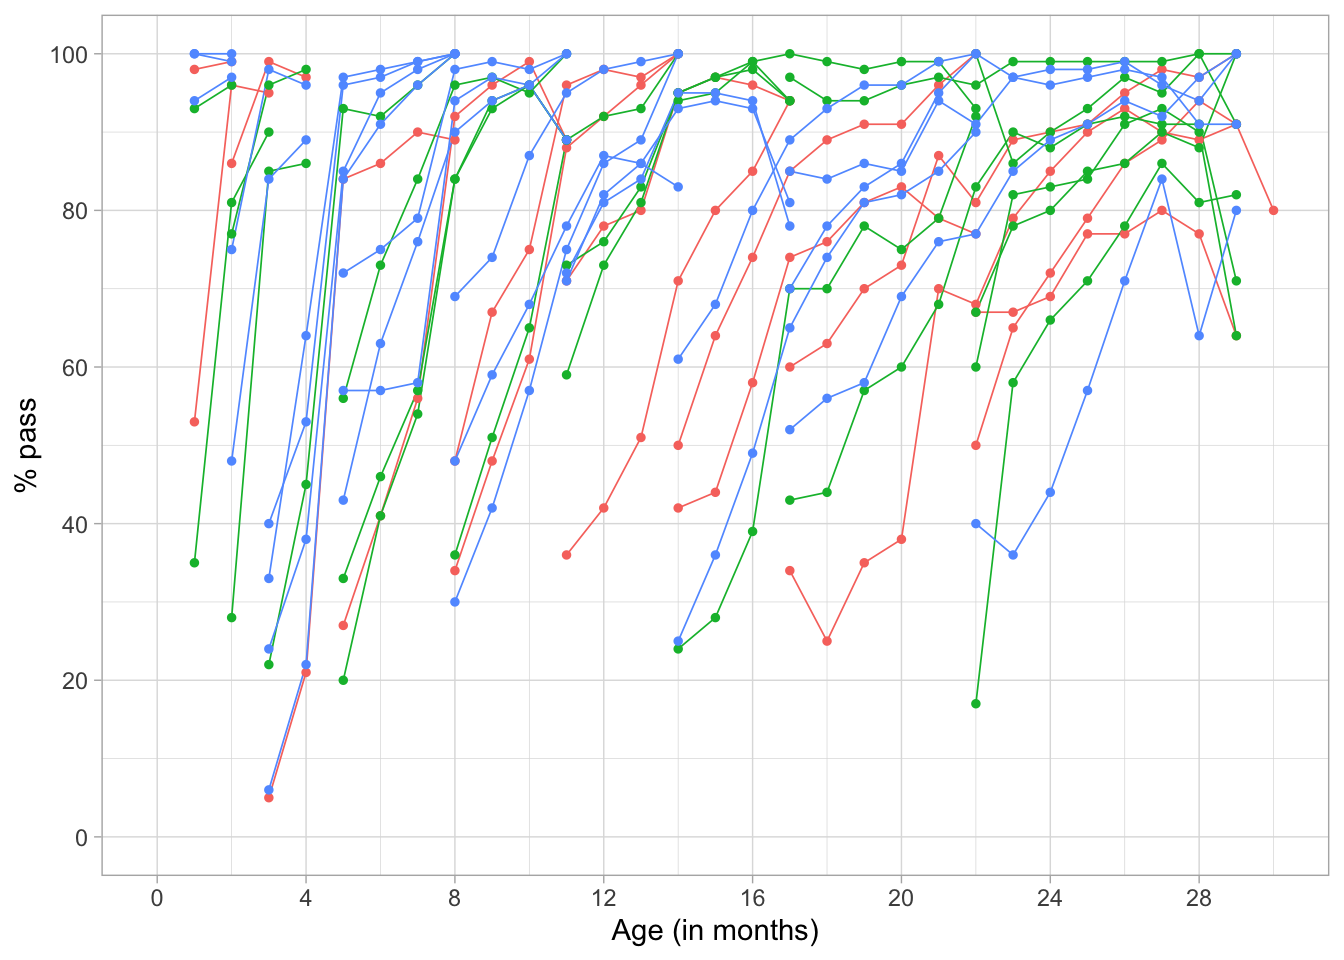
\includegraphics[width=1\linewidth]{dbook1_files/figure-latex/smoccpa-1} 

}

\caption{Empirical percentage of passing each milestone in the DDI against age (Source: SMOCC data, \(n\) = 2151, 9 occasions).}\label{fig:smoccpa}
\end{figure}



Figure \ref{fig:smoccpa} summarizes the response obtained on each milestone as a curve against age. The percentage of pass scores increases with age for all milestones. Note that curves on the left have steeper slopes than those on the right, thus indicating that development is faster for younger children.

The domain determines the coloured (blue: gross motor, green: fine motor, red: communication). In general, domains are well mixed across age, though around some ages, e.g., at four months, multiple milestones from the same domain appear.

\hypertarget{sec:probd}{%
\section{Probability of passing a milestone given D-score}\label{sec:probd}}

\begin{figure}

{\centering 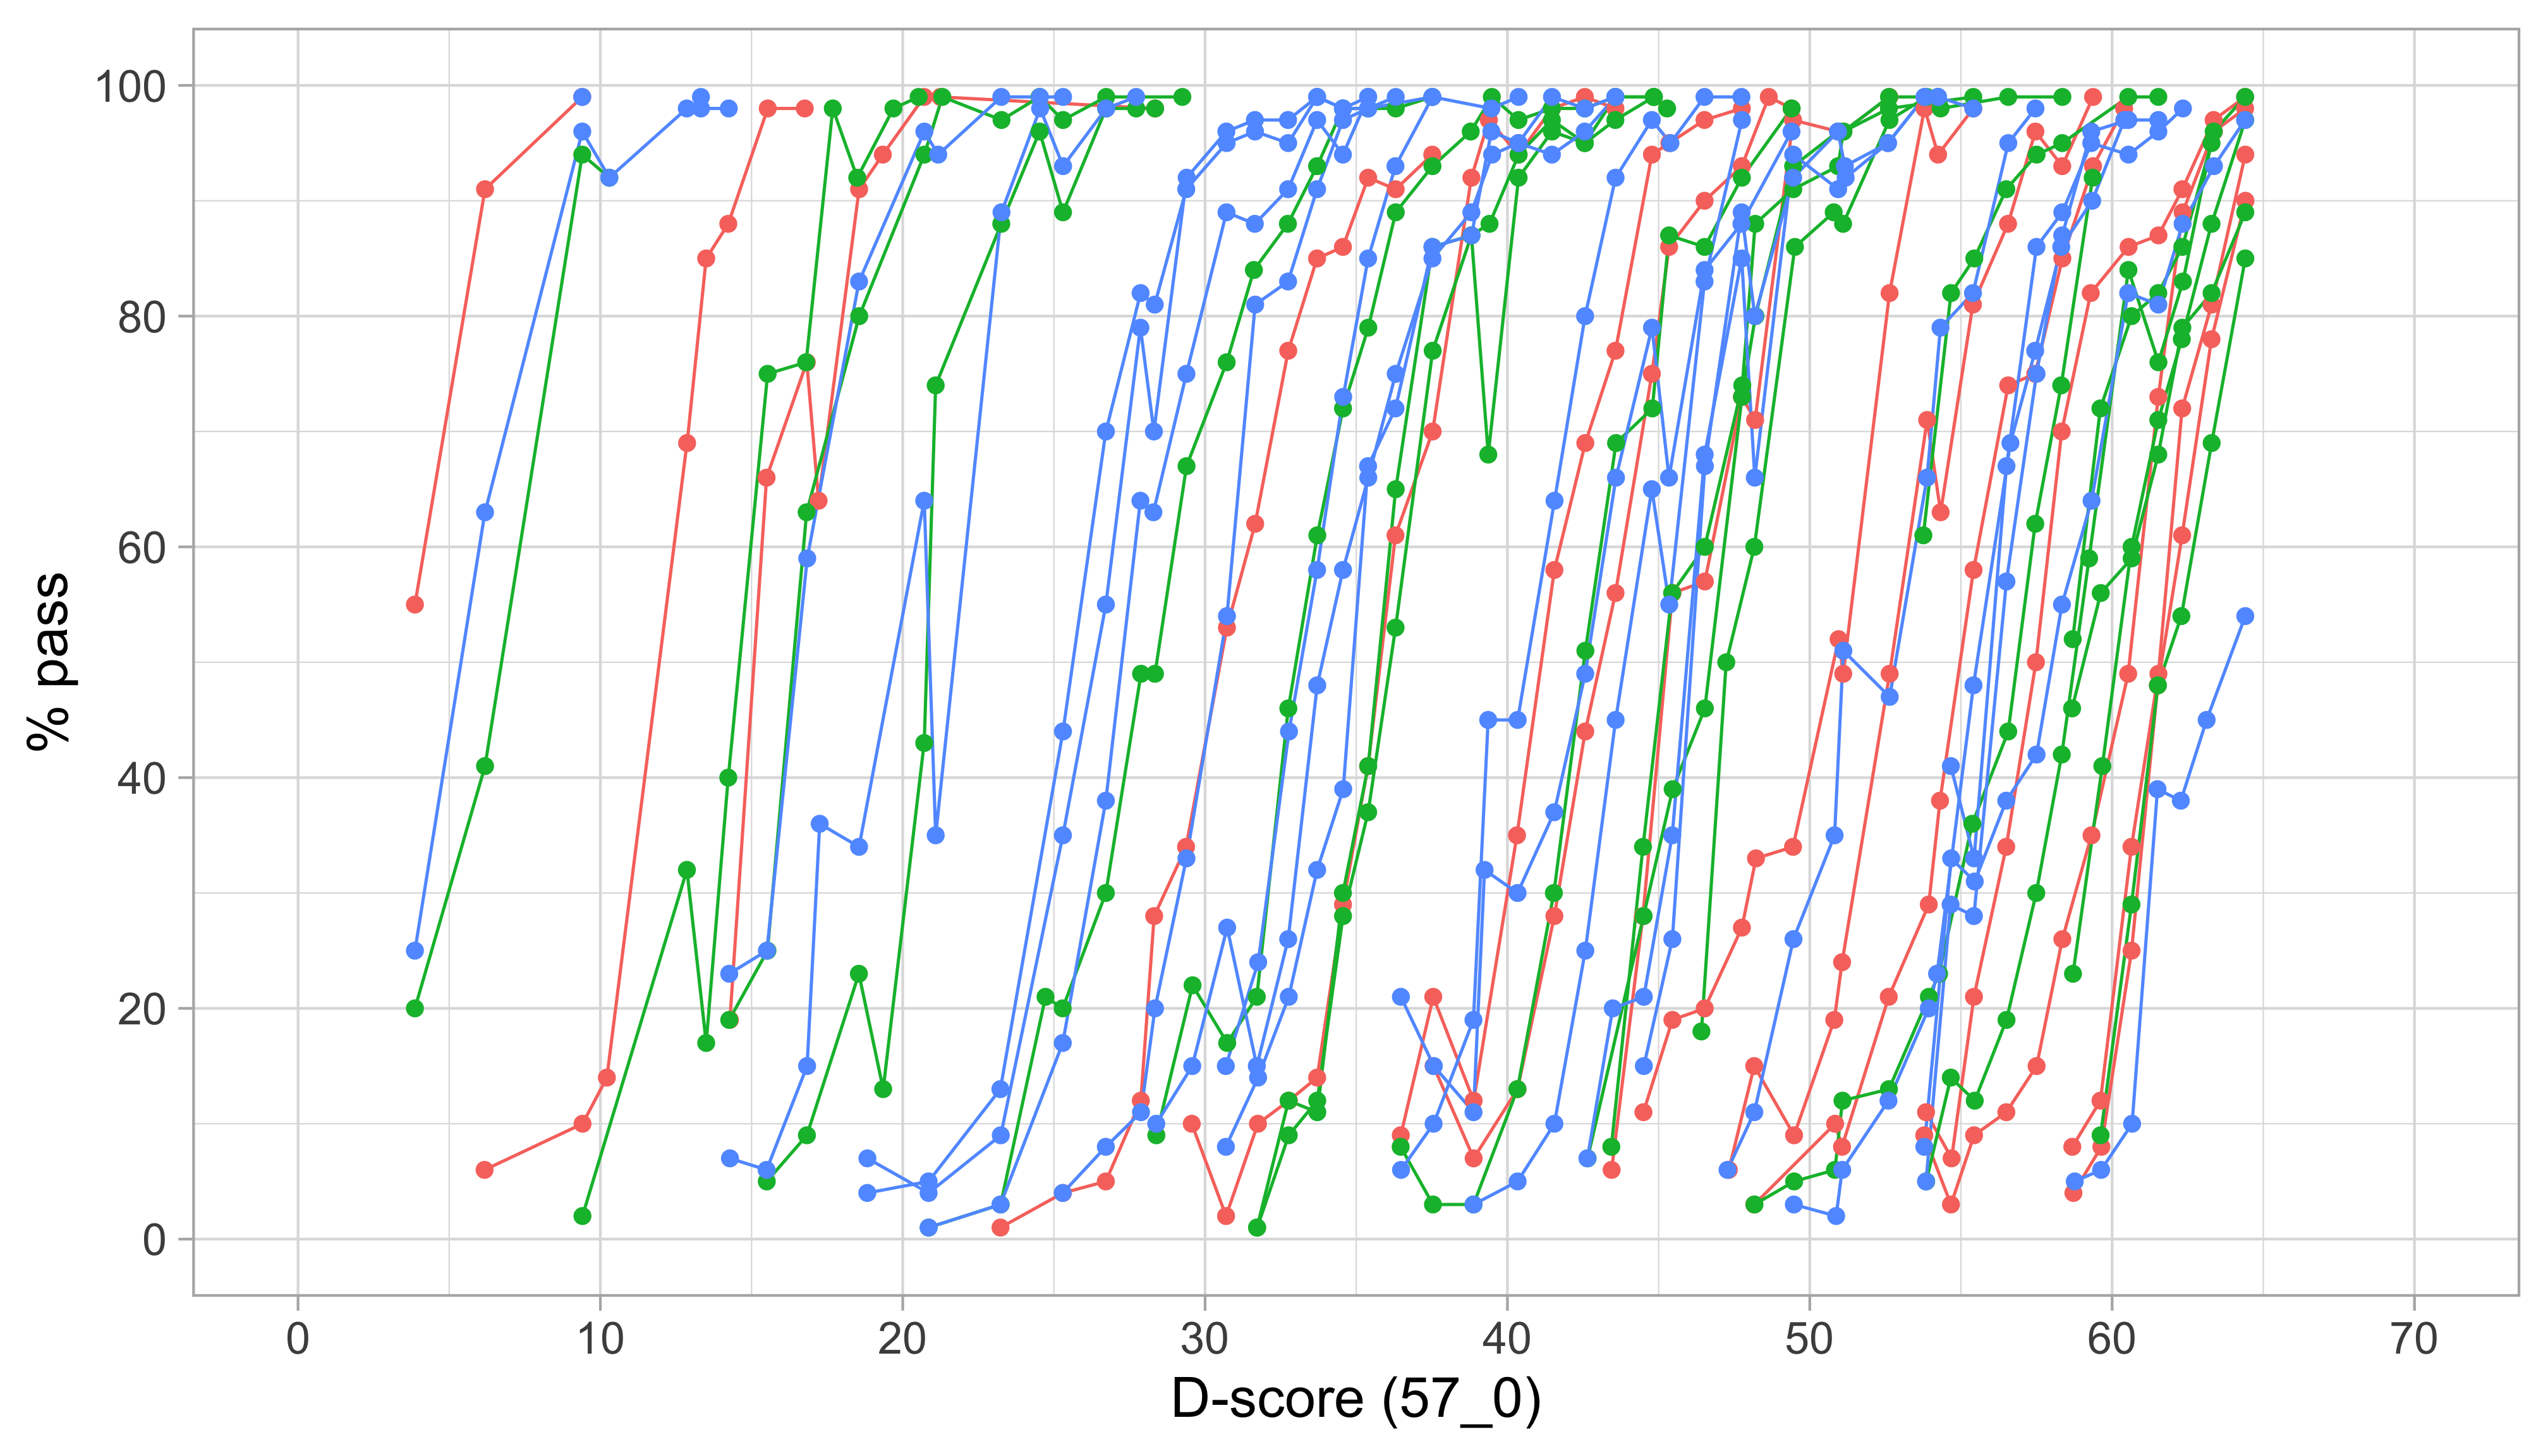
\includegraphics[width=1\linewidth]{dbook1_files/figure-latex/smoccpd-1} 

}

\caption{Empirical percentage of passing each milestone in the DDI against the D-score (Source: SMOCC data, 2151 children, 9 occasions).}\label{fig:smoccpd}
\end{figure}



Figure \ref{fig:smoccpd} is similar to Figure \ref{fig:smoccpa}, but with the horizontal axis replaced by the D-score. The D-score summarizes development into one number. See \ref{sec:dscoreestimation} for a detailed explanation on how to calculate the D-score. The vertical axis with per cent pass is unchanged.

The percentage of successes increases with D-score for all milestones. In contrast to Figure \ref{fig:smoccpa} all curves have a similar slope, a desirable property needed for an interval scale with a constant unit of measurement (c.f. Section \ref{sec:unitbased}).

How can the relation between per cent pass and age be so different from the relation between per cent pass and the D-score? The next section explains the reason.

\hypertarget{sec:aged}{%
\section{Relation between age and the D-score}\label{sec:aged}}

\begin{figure}

{\centering 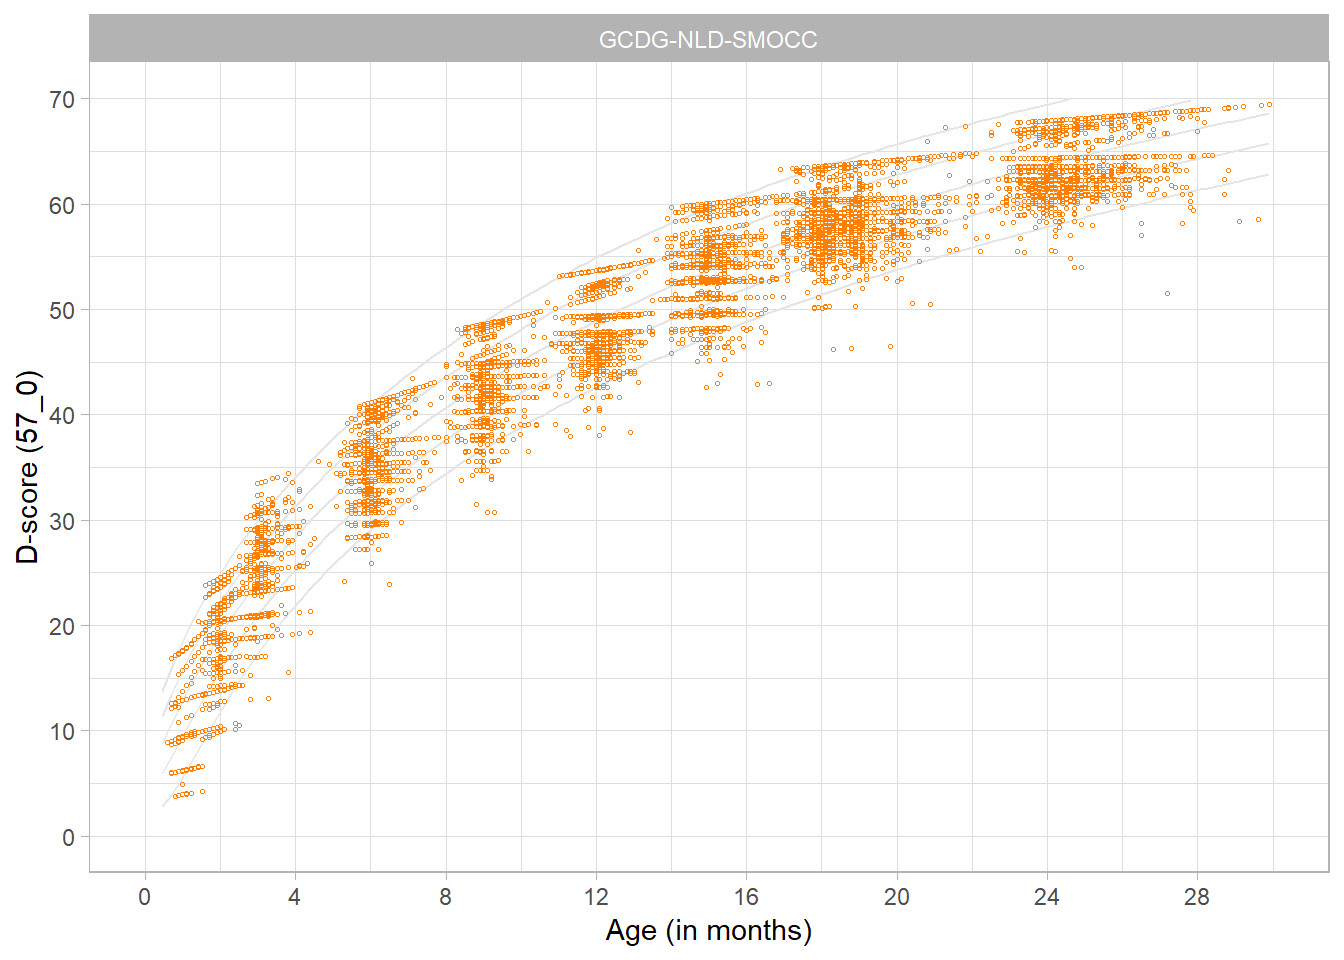
\includegraphics[width=1\linewidth]{dbook1_files/figure-latex/smoccda-1} 

}

\caption{Relation between child D-score and child age in a cohort of Dutch children (Source: SMOCC data, \(n\) = 2151, 9 occasions).}\label{fig:smoccda}
\end{figure}



Figure \ref{fig:smoccda} shows that the relation between D-score and age is nonlinear. Development in the first year is more rapid than in the second year. During the first year, infants gain about 40\(D\), whereas in the second year they gain about 20\(D\). A similar change in growth rate occurs in length (first year: 23 cm, second year: 12 cm, for Dutch children).

\begin{figure}

{\centering 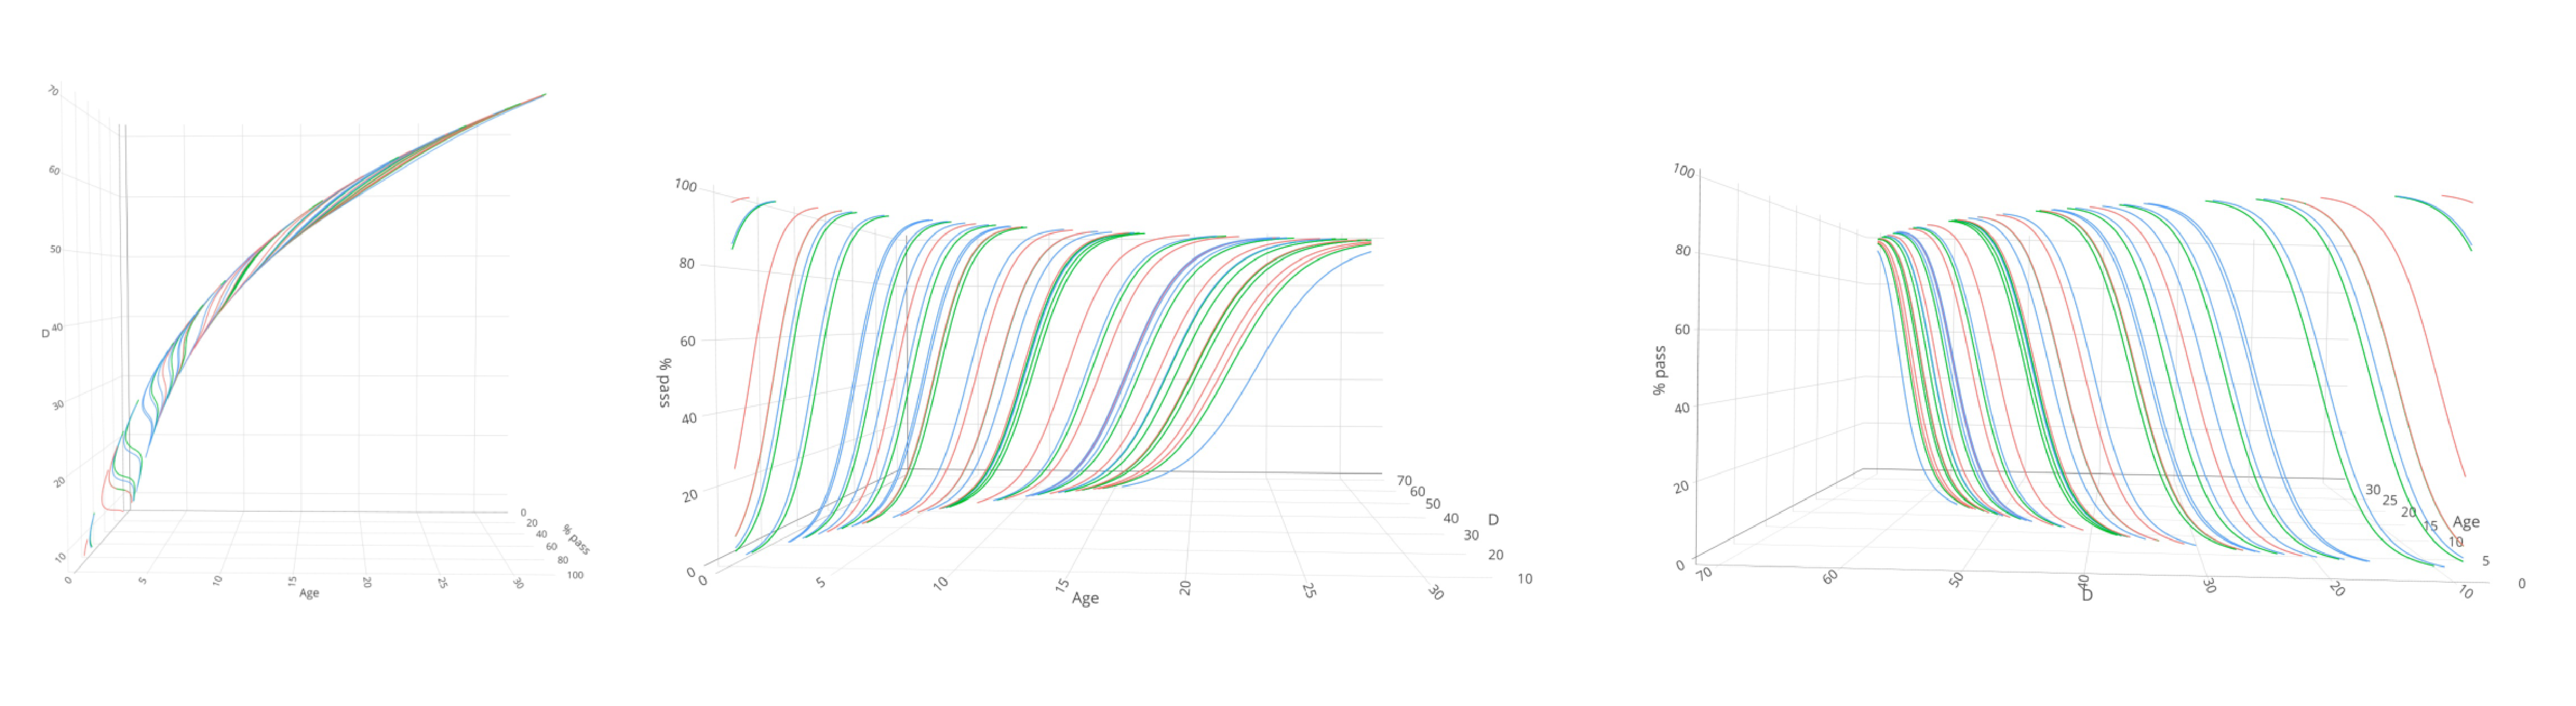
\includegraphics[width=1\linewidth]{fig/scenes} 

}

\caption{3D-line graph illustrating how the patterns in Figures \ref{fig:smoccpa} and \ref{fig:smoccpd} induce the curvature in the relation between D-score and age. The printed version shows three orientations of the relation between age, percent pass and D-score. The online version holds an interactive 3D graph that the reader can actively manipulate the orientation of the graph by click-hold-drag mouse operations.}\label{fig:smoccdap}
\end{figure}



Figure \ref{fig:smoccdap} shows the mutual relations between age, percentage of milestone passing and the D-score. There are three main orientations.

\begin{itemize}
\tightlist
\item
  In the default orientation (age on the horizontal axis, D-score on the vertical axis), we see a curvilinear relation between the age and item difficulty.
\item
  Rotate the graph (age on the horizontal axis, passing percentage on the vertical axis). Observe that this is the same pattern as in Figure \ref{fig:smoccpa} (with \emph{unequal slopes}). Curves are coloured by domain.
\item
  Rotate the graph (D-score on the horizontal axis, passing percentage on the vertical axis). Observe that this pattern is the same as in Figure \ref{fig:smoccpd} (with \emph{equal slopes}).
\end{itemize}

All patterns can co-exist because of the curvature in the relation between D-score and age. The curvature is never explicitly modelled or defined, but a consequence of the equal-slopes assumption in the relation between the D-score and the passing percentage of a milestone.

\hypertarget{sec:measurementmodel}{%
\section{Measurement model for the D-score}\label{sec:measurementmodel}}

\hypertarget{what-are-measurement-models}{%
\subsection{What are measurement models?}\label{what-are-measurement-models}}

From section \ref{sec:whatismeasurement} we quote:

\begin{quote}
The measurement model specifies the relations between the data and the latent variable.
\end{quote}

The term \emph{Item Response Theory} (IRT) refers to the scientific theory of measurement models. Good introductory works include \protect\hyperlink{ref-wright1982}{Wright and Masters} (\protect\hyperlink{ref-wright1982}{1982}), \protect\hyperlink{ref-embretsen2000}{Embretsen and Reise} (\protect\hyperlink{ref-embretsen2000}{2000}) and \protect\hyperlink{ref-engelhard2013}{Engelhard Jr.} (\protect\hyperlink{ref-engelhard2013}{2013}).

IRT models enable quantification of the locations of both \emph{items (milestones) and} persons* on the latent variable. We reserve the term \emph{item} for generic properties, and \emph{milestone} for child development. In general, items are part of the measurement instrument, persons are the objects to be measured.

An IRT model has three major structural components:

\begin{itemize}
\tightlist
\item
  Specification of the underlying \emph{latent variable(s)}. In this work, we restrict ourselves to models with just one latent variable. Multi-dimensional IRT models do have their uses, but they are complicated to fit and not widely used;
\item
  For a given item, a specification of the \emph{probability of success} given a value on the latent variables. This specification can take many forms. Section \ref{sec:itemresponsefunctions} focuses on this in more detail;
\item
  Specification how probability models for the different items should be combined. In this work, we will restrict to models that assume \emph{local independence} of the probabilities. In that case, the probability of passing two items is equal to the product of success probabilities.
\end{itemize}

\hypertarget{sec:adaptmodel}{%
\subsection{Adapt the model? Or adapt the data?}\label{sec:adaptmodel}}

The measurement model induces a predictable pattern in the observed items. We can test this pattern against the observed data. When there is misfit between the expected and observed data, we can follow two strategies:

\begin{itemize}
\tightlist
\item
  Make the measurement model more general;
\item
  Discard items (and sometimes persons) to make the model fit.
\end{itemize}

These are very different strategies that have led to heated debates among psychometricians. See \protect\hyperlink{ref-engelhard2013}{Engelhard Jr.} (\protect\hyperlink{ref-engelhard2013}{2013}) for an overview.

In this work, we opt for the - rigorous - Rasch model (\protect\hyperlink{ref-rasch1960}{Rasch} (\protect\hyperlink{ref-rasch1960}{1960})) and will adapt the data to reduce discrepancies between model and data. Arguments for this choice are given later, in Section \ref{sec:whyrasch}.

\hypertarget{sec:itemresponsefunctions}{%
\section{Item response functions}\label{sec:itemresponsefunctions}}

Most measurement models describe the probability of passing an item as a function of the \emph{difference} between the person's ability and the item's difficulty. A person with low ability will almost inevitably fail a heavy item, whereas a highly able person will almost surely pass an easy item.

Let us now introduce a few symbols. We adopt the notation used in \protect\hyperlink{ref-wright1982}{Wright and Masters} (\protect\hyperlink{ref-wright1982}{1982}). We use \(\beta_n\) (ability) to refer to the true (but unknown) developmental score of child \(n\). Symbol \(\delta_i\) (difficulty) is the true (but unknown) difficulty of an item \(i\), and \(\pi_{ni}\) is the probability that child \(n\) passes item \(i\). See Appendix A for a complete list.

The difference between the ability of child \(n\) and difficulty of item \(i\) is

\[\beta_n - \delta_i\]

In the special case that \(\beta_n = \delta_i\), the person will have a probability of 0.5 of passing the item.

\hypertarget{logistic-model}{%
\subsection{Logistic model}\label{logistic-model}}

A widely used method is to express differences on the latent scale in terms of \emph{logistic units} (or \emph{logits}) (\protect\hyperlink{ref-berkson1944}{Berkson 1944}). The reason preferring the logistic over the linear unit is that its output returns a probability value that maps to discrete events. In our case, we can describe the probability of passing an item (milestone) as a function of the difference between \(\beta_n\) and \(\delta_i\) expressed in logits.

\begin{figure}

{\centering 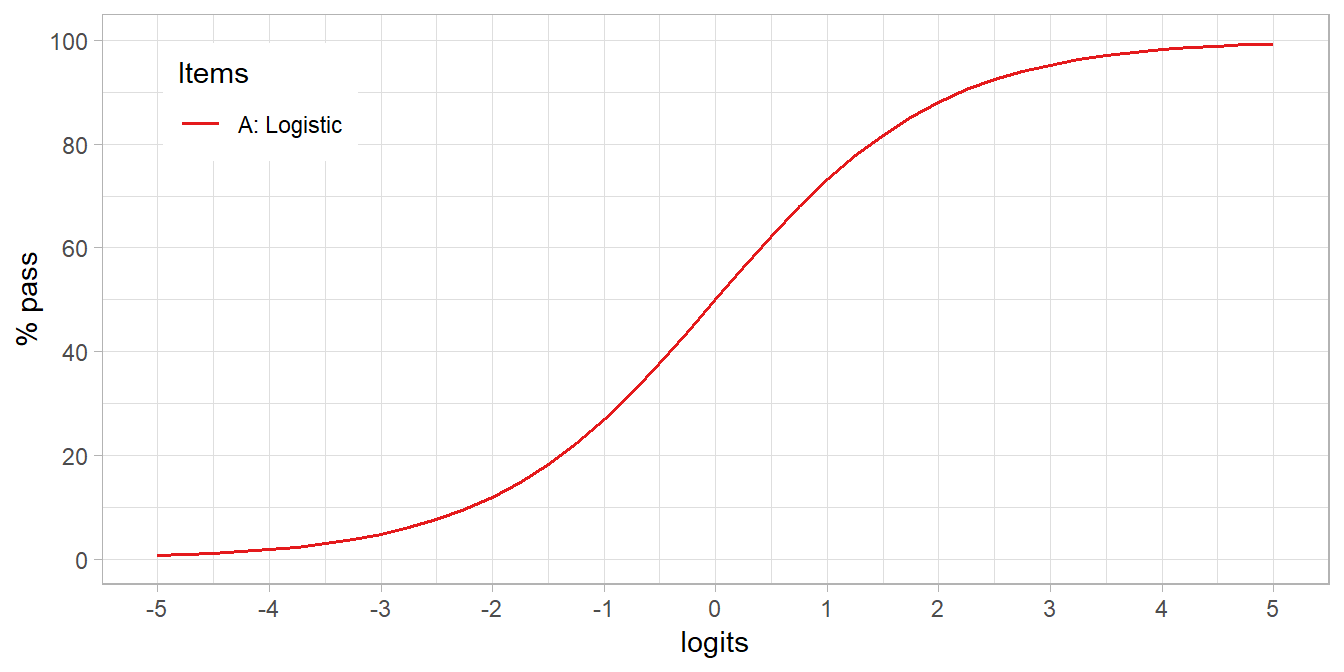
\includegraphics[width=1\linewidth]{dbook1_files/figure-latex/logisticplot-1} 

}

\caption{Standard logistic curve. Percentage of children passing an item for a given ability-difficulty gap \(\beta_n - \delta_i\).}\label{fig:logisticplot}
\end{figure}



Figure \ref{fig:logisticplot} shows how the percentage of children that pass the item varies in terms of the ability-difficulty gap \(\beta_n - \delta_i\). The gap can vary either by \(\beta_n\) or \(\delta_i\) so that we may use the graph in two ways:

\begin{itemize}
\tightlist
\item
  To find the probability of passing items with various difficulties for a child with ability \(\beta_n\). If \(\delta_i = \beta_n\) then \(\pi_{ni} = 0.5\). If \(\delta_i < \beta_n\) then \(\pi_{ni} > 0.5\), and if \(\delta_i > \beta_n\) then \(\pi_{ni} < 0.5\). In words: If the difficulty of the item is equal to the child's ability, then the child has a 50/50 chance to pass. The child will have a higher than 50/50 chance of passing for items with lower difficulty and have a lower than 50/50 chance of passing for items with difficulties that exceed the child's ability.
\item
  To find the probability of passing a given item \(\delta_i\) for children that vary in ability. If \(\beta_n < \delta_i\) then \(\pi_{ni} < 0.5\), and if \(\beta_n > \delta_i\) then \(\pi_{ni} > 0.5\). In words: Children with abilities lower than the item's difficulty will have lower than 50/50 chance of passing, whereas children with abilities that exceed the item's difficulty will have a higher than 50/50 chance of passing.
\end{itemize}

Formula \eqref{eq:logistic} defines the standard logistic curve:

\begin{equation}
\pi_{ni} = \frac{\exp(\beta_n - \delta_i)}{1+\exp(\beta_n -\delta_i)} \label{eq:logistic}
\end{equation}

One way to interpret the formula is as follows. The logarithm of the odds that a person with ability \(\beta_n\) passes an item of difficulty \(\delta_i\) is equal to the difference \(\beta_n-\delta_i\) (\protect\hyperlink{ref-wright1982}{Wright and Masters 1982}). For example, suppose that the probability that person \(n\) passes milestone \(i\) is \(\pi_{ni} = 0.5\). In that case, the odds of passing is equal to \(0.5 / (1-0.5) = 1\), so \(\log(1) = 0\) and thus \(\beta_n = \delta_i\). If \(\beta_n - \delta_i = \log(2) = 0.693\) person \(n\) is \emph{two} times more likely to pass than to fail. Likewise, if the difference is \(\beta_n - \delta_i = \log(3) = 1.1\), then person \(n\) is \emph{three} more likely to pass. And so on.

\hypertarget{types-of-item-response-functions}{%
\subsection{Types of item response functions}\label{types-of-item-response-functions}}

The standard logistic function is by no means the only option to map the relationship between the latent variable and the probability of passing an item. The logistic function is the dominant choice in IRT, but it is instructive to study some other mappings. The \emph{item response function} maps success probability against ability.

\begin{figure}

{\centering 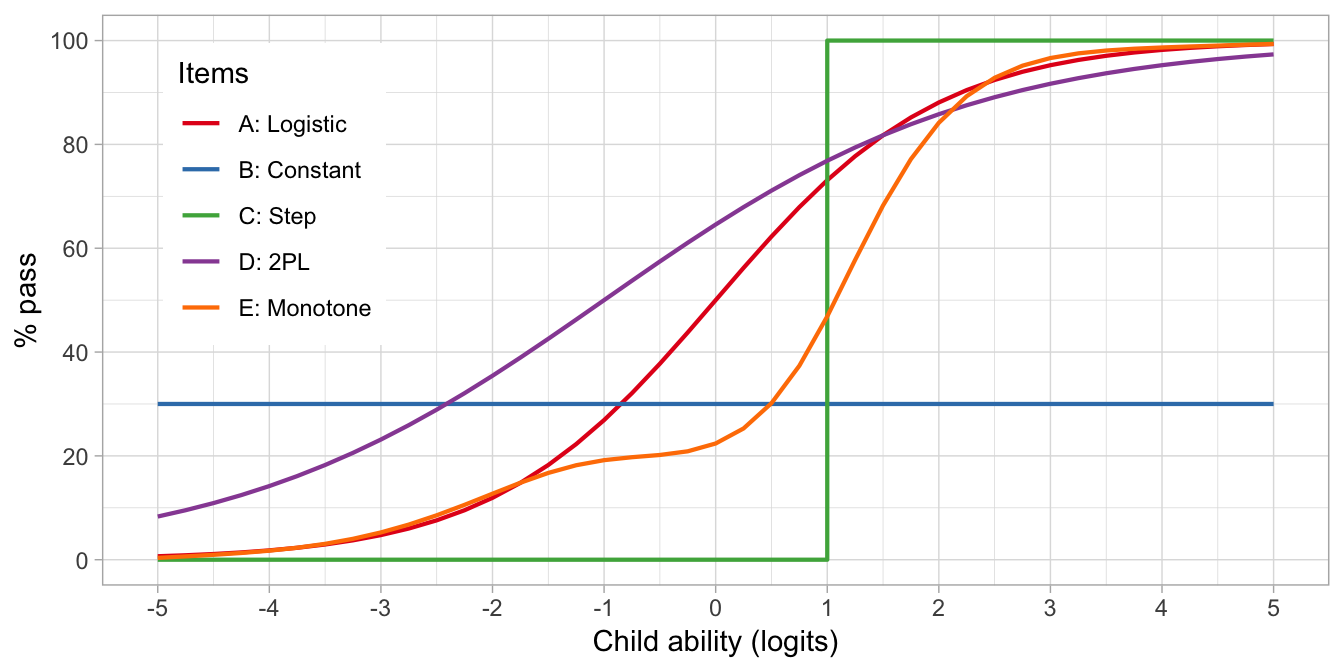
\includegraphics[width=1\linewidth]{dbook1_files/figure-latex/irfplot-1} 

}

\caption{Item response functions for five hypothetical items, each demonstrating a positive relation between ability and probability to pass.}\label{fig:irfplot}
\end{figure}



Figure \ref{fig:irfplot} illustrates several other possibilities. Let us consider five hypothetical items, A-E. Note that the horizontal axis now refers to the ability, instead of the ability-item gap in \ref{fig:logisticplot}.

\begin{itemize}
\tightlist
\item
  A: Item A is the logistic function discussed in Section \ref{sec:itemresponsefunctions}.
\item
  B: For item B, the probability of passing is constant at 30 per cent. This 30 per cent is not related to ability. Item B does not measure ability, only adds to the noise, and is of low quality.
\item
  C: Item C is a step function centred at an ability level of 1, so \emph{all} children with an ability below 1 logit fail and \emph{all} children with ability above 1 logit pass. Item C is the ideal item for discriminating children with abilities above and below 1. The item is not sensitive to differences at other ability levels, and often not so realistic in practice.
\item
  D: Like A, item D is a smoothly increasing logistic function, but it has an extra parameter that allows it to vary its slope (or discrimination). The extra parameter can make the curve steeper (more discriminatory) than the red curve, in the limit approaching a step curve. It can also become shallower (less discriminatory) than the red curve (as plotted here), in the limit approaching a constant curve (item B). Thus, item D generalizes items A, B or C.
\item
  E: Item E is even more general in the sense that it need not be logistic, but a general monotonically increasing function. As plotted, the item is insensitive to abilities between -1 and 0 logits, and more sensitive to abilities between 0 to 2 logits.
\end{itemize}

These are just some examples of how the relationship between the child's ability and passing probability could look. In practice, the curves need not start at 0 per cent or end at 100 per cent. They could also be U-shaped, or have other non-monotonic forms. See \protect\hyperlink{ref-coombs1964}{Coombs} (\protect\hyperlink{ref-coombs1964}{1964}) for a thorough overview of such models. In practice, most models are restricted to shapes A-D.

\hypertarget{person-response-functions}{%
\subsection{Person response functions}\label{person-response-functions}}

We can reverse the roles of persons and items. The \emph{person response function} tells us how likely it is that a single person can pass an item, or more commonly, a set of items.

Let us continue with items A, C and D from Figure \ref{fig:irfplot}, and calculate the response function for three children, respectively with abilities \(\beta_1 = -2\), \(\beta_2 = 0\) and \(\beta_3 = 2\).

\begin{figure}

{\centering 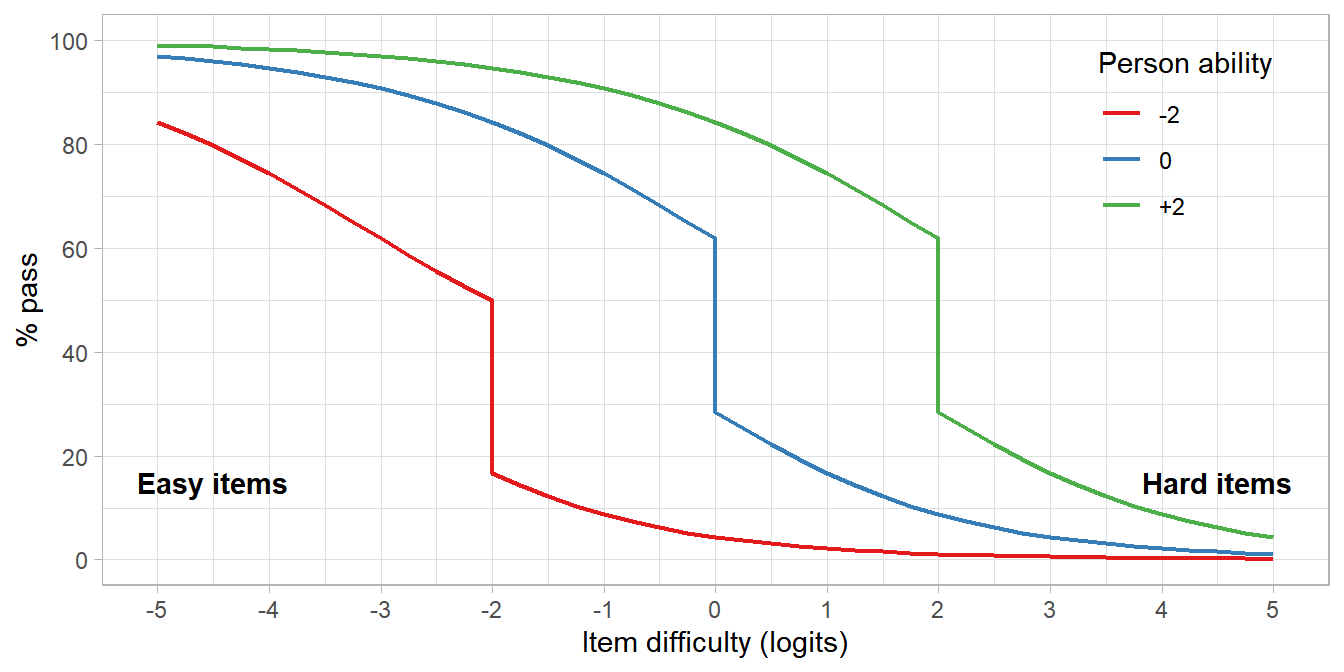
\includegraphics[width=1\linewidth]{dbook1_files/figure-latex/prfplot-1} 

}

\caption{Person response functions for three children with abilities -2, 0 and +2, using a small test of items A, C and D.}\label{fig:prfplot}
\end{figure}



Figure \ref{fig:prfplot} presents the person response functions from three persons with abilities of -2, 0 and +2 logits. We calculate the functions as the average of response probabilities on items A, C and D. Thus, on average, we expect that child 1 logit will pass an easy item of difficulty -3 in about 60 per cent of the time, whereas for an intermediate item of difficulty of -1 the passing probability would be 10 per cent. For child 3, with higher ability, these probabilities are quite different: 97\% and 90\%. The substantial drop in the middle of the curve is due to the step function of item A.

\hypertarget{sec:engelhard}{%
\section{Engelhard criteria for invariant measurement}\label{sec:engelhard}}

In this work, we strive to achieve \emph{invariant measurement}, a strict form of measurements that is subject to the following requirements (\protect\hyperlink{ref-engelhard2013}{Engelhard Jr. 2013, 14}):

\begin{enumerate}
\def\labelenumi{\arabic{enumi}.}
\tightlist
\item
  \emph{Item-invariant measurement of persons}: The measurement of persons must be independent of the particular items used for the measuring.
\item
  \emph{Non-crossing person response functions}: A more able person must always have a better chance of success on an item that a less able person.
\item
  \emph{Person-invariant calibration of test items}: The calibration of the items must be independent of the particular persons used for calibration.
\item
  \emph{Non-crossing item response functions}: Any person must have a better chance of success on an easy item than on a more difficult item.
\item
  \emph{Unidimensionality}: Items and persons take on values on a \emph{single} latent variable. Under this assumption, the relations between the items are fully explainable by the scores on the latent scale. In practice, the requirement implies that items should measure the same construct. (\protect\hyperlink{ref-hattie1985}{Hattie 1985})
\end{enumerate}

Three families of IRT models support invariant measurement:

\begin{enumerate}
\def\labelenumi{\arabic{enumi}.}
\tightlist
\item
  Scalogram model (\protect\hyperlink{ref-guttman1950}{Guttman 1950})
\item
  Rasch model (\protect\hyperlink{ref-rasch1960}{Rasch 1960}; \protect\hyperlink{ref-andrich1978}{Andrich 1978}; \protect\hyperlink{ref-wright1982}{Wright and Masters 1982})
\item
  Mokken scaling model (\protect\hyperlink{ref-mokken1971}{Mokken 1971}; \protect\hyperlink{ref-molenaar1997}{Molenaar 1997})
\end{enumerate}

The Guttman and Mokken models yield an ordinal latent scale, while the Rasch model yields an interval scale (with a constant unit).

\hypertarget{sec:whyrasch}{%
\section{Why take the Rasch model?}\label{sec:whyrasch}}

\begin{itemize}
\tightlist
\item
  \emph{Invariant measurement}: The Rasch model meets the five Engelhard criteria (c.f. Section \ref{sec:engelhard}).
\item
  \emph{Interval scale}: When it fits, the Rasch model provides an interval scale, the de-facto requirement for any numerical comparisons (c.f. Section \ref{sec:motivationunit}).
\item
  \emph{Parsimonious}: The Rasch model has one parameter for each item and one parameter for each person. The Rash model one of the most parsimonious IRT models, and can easily be applied to thousands of items and millions of persons.
\item
  \emph{Specific objectivity}: Person and item parameters are mathematically separate entities in the Rasch model. In practice, this means that the estimated difference in ability between two persons does not depend on the difficulty of the test. Also, the estimated differences in difficulties between two items do not depend on the abilities in the calibration sample. The property is especially important in the analysis of combined data, where abilities can vary widely between sources. See \protect\hyperlink{ref-rasch1977}{Rasch} (\protect\hyperlink{ref-rasch1977}{1977}) for derivations and examples.
\item
  \emph{Unified model}: The Rasch model unifies distinct traditions in measurement theory. One may derive the Rasch model from

  \begin{itemize}
  \tightlist
  \item
    \href{https://www.rasch.org/rmt/rmt143g.htm}{Thorndike's 1904 criteria}
  \item
    \href{https://www.rasch.org/rmt/rmt63e.htm}{Guttman scalogram model}
  \item
    \href{https://www.rasch.org/rmt/rmt62c.htm}{Ratio-scale counts}
  \item
    \href{https://www.rasch.org/rmt/rmt32e.htm}{Raw scores as sufficient statistics}
  \item
    \href{https://www.rasch.org/rmt/rmt21a.htm}{Thurstone's scaling requirements}
  \item
    \href{https://www.rasch.org/rmt/rmt21b.htm}{Campbell concatenation}
  \item
    \href{https://www.rasch.org/rmt/rmt11a.htm}{Rasch's specific objectivity}
  \end{itemize}
\item
  \emph{Fits child development data}: Last but not least, as we will see in Section \ref{ch:evaluation}, the Rasch model provides an excellent fit to child development milestones.
\end{itemize}

\newpage

\hypertarget{ch:computation}{%
\chapter{Computation}\label{ch:computation}}

This section explains the basic computations needed for fitting and evaluating the Rasch model. We distinguish the following steps:

\begin{itemize}
\tightlist
\item
  Identify nature of the problem (\ref{sec:datapreparation})
\item
  Estimation of item parameters (\ref{sec:itemestimation})
\item
  Anchoring (\ref{sec:anchoring})
\item
  Estimation of the D-score (\ref{sec:dscoreestimation})
\item
  Estimation of age-conditional references (\ref{sec:reference})
\end{itemize}

Readers not interested in these details may continue to model evaluation in Section \ref{ch:evaluation}.

\hypertarget{sec:datapreparation}{%
\section{Identify nature of the problem}\label{sec:datapreparation}}

The SMOCC dataset, introduced in Section \ref{sec:smocc}, contains scores on the DDI of Dutch children aged 0-2 years made during nine visits.

\begin{landscape}\begin{table}

\caption{\label{tab:smocctable}SMOCC DDI milestones, first three children, 0-2 years.}
\centering
\resizebox{\linewidth}{!}{
\begin{tabu} to \linewidth {>{}r>{}r>{}r>{}r>{}r>{}r>{}r>{}r>{}r>{}r>{}r>{}r>{}r>{}r>{}r>{}r>{}r>{}r>{}r>{}r>{}r>{}r>{}r>{}r>{}r>{}r>{}r>{}r>{}r>{}r>{}r>{}r>{}r>{}r>{}r>{}r>{}r>{}r>{}r>{}r>{}r>{}r>{}r>{}r>{}r>{}r>{}r>{}r>{}r>{}r>{}r>{}r>{}r>{}r>{}r>{}r>{}r}
\toprule
29 & 30 & 31 & 33 & 34 & 36 & 37 & 39 & 41 & 43 & 44 & 16 & 36 & 41 & 48 & 01 & 02 & 03 & 04 & 05 & 07 & 08 & 09 & 10 & 11 & 12 & 13 & 14 & 15 & 16 & 17 & 18 & 19 & 54 & 06 & 52 & 53 & 54 & 55 & 56 & 57 & 58 & 59 & 60 & 61 & 62 & 63 & 64 & 65 & 66 & 67 & 68 & 69 & 70 & 71 & 46 & 68\\
\midrule
1 & 0 &  &  &  &  &  &  &  &  &  &  &  &  &  & 1 & 0 &  &  &  &  &  &  &  &  &  &  &  &  &  &  &  &  &  &  & 1 & 1 &  &  & 1 &  &  &  &  &  &  &  &  &  &  &  &  &  &  &  &  \vphantom{1} & \\
 & 1 &  &  &  &  &  &  &  &  &  &  &  &  &  &  & 1 &  &  &  &  &  &  &  &  &  &  &  &  &  &  &  &  &  &  &  &  &  &  &  &  &  &  &  &  &  &  &  &  &  &  &  &  &  &  &  \vphantom{1} & \\
 &  & 1 &  &  &  &  &  &  &  &  & 0 &  &  &  &  &  & 1 & 1 & 0 &  &  &  &  &  &  &  &  &  &  &  &  &  &  & 0 &  &  & 1 & 1 &  & 1 & 1 & 1 &  &  &  &  &  &  &  &  &  &  &  &  &  & \\
 &  &  & 0 &  &  &  &  &  &  &  & 1 &  &  &  &  &  &  &  & 1 & 1 & 0 & 1 &  &  &  &  &  &  &  &  &  &  &  & 1 &  &  &  & 1 &  &  & 1 & 1 & 0 & 1 & 1 &  &  &  &  &  &  &  &  &  &  & \\
 &  &  & 1 &  &  &  &  &  &  &  &  &  &  &  &  &  &  &  &  & 1 & 0 & 1 &  &  &  &  &  &  &  &  &  &  &  &  &  &  &  &  &  &  &  &  & 1 & 1 & 1 & 1 &  &  &  &  &  &  &  &  &  & \\
\addlinespace
 &  &  &  & 1 & 1 & 1 &  &  &  &  &  & 1 &  &  &  &  &  &  &  &  &  &  & 1 &  &  &  &  &  &  &  &  &  &  &  &  &  &  &  &  &  &  &  &  &  &  & 1 & 0 & 1 &  &  &  &  &  &  &  & \\
 &  &  &  &  &  & 1 &  &  &  &  &  & 1 &  &  &  &  &  &  &  &  &  &  &  & 1 & 1 &  &  &  &  &  &  &  &  &  &  &  &  &  &  &  &  &  &  &  &  &  &  &  & 0 & 0 &  &  &  &  &  & \\
 &  &  &  &  &  &  & 1 &  &  &  &  &  &  &  &  &  &  &  &  &  &  &  &  &  &  & 0 & 1 &  &  &  &  &  &  &  &  &  &  &  &  &  &  &  &  &  &  &  &  &  &  &  & 0 & 0 &  &  &  & \\
 &  &  &  &  &  &  &  & 1 &  &  &  &  &  & 1 &  &  &  &  &  &  &  &  &  &  &  &  &  &  & 1 &  &  &  &  &  &  &  &  &  &  &  &  &  &  &  &  &  &  &  &  &  &  &  &  &  & 0 & 1\\
1 & 1 &  &  &  &  &  &  &  &  &  &  &  &  &  & 1 & 1 &  &  &  &  &  &  &  &  &  &  &  &  &  &  &  &  &  &  & 1 & 1 &  &  & 1 &  &  &  &  &  &  &  &  &  &  &  &  &  &  &  &  & \\
\addlinespace
 & 1 &  &  &  &  &  &  &  &  &  &  &  &  &  &  & 1 &  &  &  &  &  &  &  &  &  &  &  &  &  &  &  &  &  &  &  &  &  &  &  &  &  &  &  &  &  &  &  &  &  &  &  &  &  &  &  & \\
 &  & 1 &  &  &  &  &  &  &  &  & 0 &  &  &  &  &  & 1 & 1 & 0 &  &  &  &  &  &  &  &  &  &  &  &  &  &  & 0 &  &  & 1 & 0 &  & 1 & 0 & 0 &  &  &  &  &  &  &  &  &  &  &  &  &  & \\
 &  &  & 0 &  &  &  &  &  &  &  & 1 &  &  &  &  &  &  &  & 1 & 0 & 0 & 1 &  &  &  &  &  &  &  &  &  &  &  & 1 &  &  &  & 1 &  &  & 1 & 0 & 1 & 0 & 1 &  &  &  &  &  &  &  &  &  &  & \\
 &  &  & 1 &  &  &  &  &  &  &  &  &  &  &  &  &  &  &  &  & 1 & 1 & 1 &  &  &  &  &  &  &  &  &  &  &  &  &  &  &  &  &  &  &  &  & 1 & 1 & 1 & 0 &  & 1 &  &  &  &  &  &  &  & \\
 &  &  &  & 1 & 1 &  &  &  &  &  &  &  &  &  &  &  &  &  &  &  &  &  & 1 & 1 &  &  &  &  &  &  &  &  &  &  &  &  &  &  &  &  &  &  &  &  &  & 1 & 1 & 1 & 1 & 1 &  &  &  &  &  & \\
\addlinespace
 &  &  &  &  &  &  &  & 1 &  & 1 &  &  &  & 1 &  &  &  &  &  &  &  &  &  &  &  &  &  & 1 & 1 &  & 1 &  & 1 &  &  &  &  &  &  &  &  &  &  &  &  &  &  &  &  &  &  &  & 1 &  & 1 & 1\\
 &  &  &  &  &  &  & 1 &  &  &  &  &  &  &  &  &  &  &  &  &  &  &  &  &  &  & 0 & 1 &  &  &  &  &  &  &  &  &  &  &  &  &  &  &  &  &  &  &  &  &  &  &  & 1 &  &  &  &  & \\
1 & 0 &  &  &  &  &  &  &  &  &  &  &  &  &  & 1 & 0 &  &  &  &  &  &  &  &  &  &  &  &  &  &  &  &  &  &  & 1 & 1 &  &  & 1 &  &  &  &  &  &  &  &  &  &  &  &  &  &  &  &  & \\
 & 1 &  &  &  &  &  &  &  &  &  &  &  &  &  &  & 0 &  &  &  &  &  &  &  &  &  &  &  &  &  &  &  &  &  &  &  &  &  &  &  &  &  &  &  &  &  &  &  &  &  &  &  &  &  &  &  & \\
 &  & 1 &  &  &  &  &  &  &  &  & 0 &  &  &  &  &  & 1 & 1 & 0 &  &  &  &  &  &  &  &  &  &  &  &  &  &  & 0 &  &  & 1 & 0 &  & 1 & 1 & 0 &  &  &  &  &  &  &  &  &  &  &  &  &  & \\
\addlinespace
 &  &  & 1 &  &  &  &  &  &  &  & 1 &  &  &  &  &  &  &  & 1 & 0 & 0 & 1 &  &  &  &  &  &  &  &  &  &  &  & 0 &  &  &  & 1 &  &  & 1 & 1 & 1 & 1 & 1 &  &  &  &  &  &  &  &  &  &  & \\
 &  &  & 1 & 1 &  &  &  &  &  &  &  &  &  &  &  &  &  &  &  & 1 & 1 & 1 &  &  &  &  &  &  &  &  &  &  &  &  &  &  &  &  &  &  &  &  & 1 & 1 & 1 & 0 & 0 &  &  &  &  &  &  &  &  & \\
 &  &  &  & 1 & 1 &  &  &  &  &  &  &  &  &  &  &  &  &  &  &  &  &  & 1 &  &  &  &  &  &  &  &  &  &  &  &  &  &  &  &  &  &  &  &  &  &  & 1 & 1 & 0 &  &  &  &  &  &  &  & \\
 &  &  &  &  &  & 0 &  &  &  &  &  & 0 &  &  &  &  &  &  &  &  &  &  &  & 1 & 1 &  &  &  &  &  &  &  &  &  &  &  &  &  &  &  &  &  &  &  &  &  &  &  & 1 & 1 &  &  &  &  &  & \\
 &  &  &  &  &  &  & 1 &  &  &  &  &  & 1 &  &  &  &  &  &  &  &  &  &  &  &  & 0 & 1 &  & 1 &  &  &  &  &  &  &  &  &  &  &  &  &  &  &  &  &  &  &  &  &  & 1 & 0 & 1 &  &  & 1\\
\addlinespace
 &  &  &  &  &  &  &  & 1 & 1 & 1 &  &  &  & 1 &  &  &  &  &  &  &  &  &  &  &  &  &  & 1 & 1 &  & 1 & 1 & 1 &  &  &  &  &  &  &  &  &  &  &  &  &  &  &  &  &  &  &  & 1 &  & 1 & 1\\
\bottomrule
\end{tabu}}
\end{table}
\end{landscape}

Table \ref{tab:smocctable} contains data of three children, measured on nine visits between ages 0 - 2 years. The DDI scores take values 0 (FAIL) and 1 (PASS). In order to save horizontal space, we truncated the column headers to the last two digits of the item names.

Since the selection of milestones depends on age, the dataset contains a large number of empty cells. Naive use of sum scores as a proxy to ability is therefore problematic. An empty cell is not a FAIL, so it is incorrect to impute those cells by zeroes.

Note that some rows contain only 1's, e.g., in row 2. Many computer programs for Rasch analysis routinely remove such \emph{perfect scores} before fitting. However, unless the number of perfect scores is very small, this is not recommended because doing so can severely affect the ability distribution.

In order to effectively handle the missing data and to preserve all persons in the analysis we separate estimation of item difficulties (c.f. section \ref{sec:itemestimation}) and person abilities (c.f. section \ref{sec:dscoreestimation}).

\hypertarget{sec:itemestimation}{%
\section{Item parameter estimation}\label{sec:itemestimation}}

\hypertarget{pairwise-estimation-of-item-difficulties}{%
\subsection{Pairwise estimation of item difficulties}\label{pairwise-estimation-of-item-difficulties}}

There are many methods for estimating the difficulty parameters of the Rasch estimation. See \protect\hyperlink{ref-linacre2004}{Linacre} (\protect\hyperlink{ref-linacre2004}{2004}) for an overview.

We will use the pairwise estimation method. This method writes the probability that child \(n\) passes item \(i\) but not item \(j\) given that the child passed one of them as \(\exp(\delta_i) / (\exp(\delta_i) + \exp(\delta_j))\). The method optimizes the pseudo-likelihood of all item pairs over the difficulty estimates by a simple iterative procedure.

\protect\hyperlink{ref-zwinderman1995}{Zwinderman} (\protect\hyperlink{ref-zwinderman1995}{1995}) has shown that this procedure provides consistent estimates with similar efficiency computationally more-intensive conditional and marginal maximum likelihood methods.

The beauty of the method is that it is independent of the ability distribution, so there is no need to remove perfect scores. We use the function \texttt{rasch.pairwise.itemcluster()} as implemented in the \texttt{sirt} package (\protect\hyperlink{ref-robitzsch2016}{Robitzsch 2016}).

\begin{figure}

{\centering 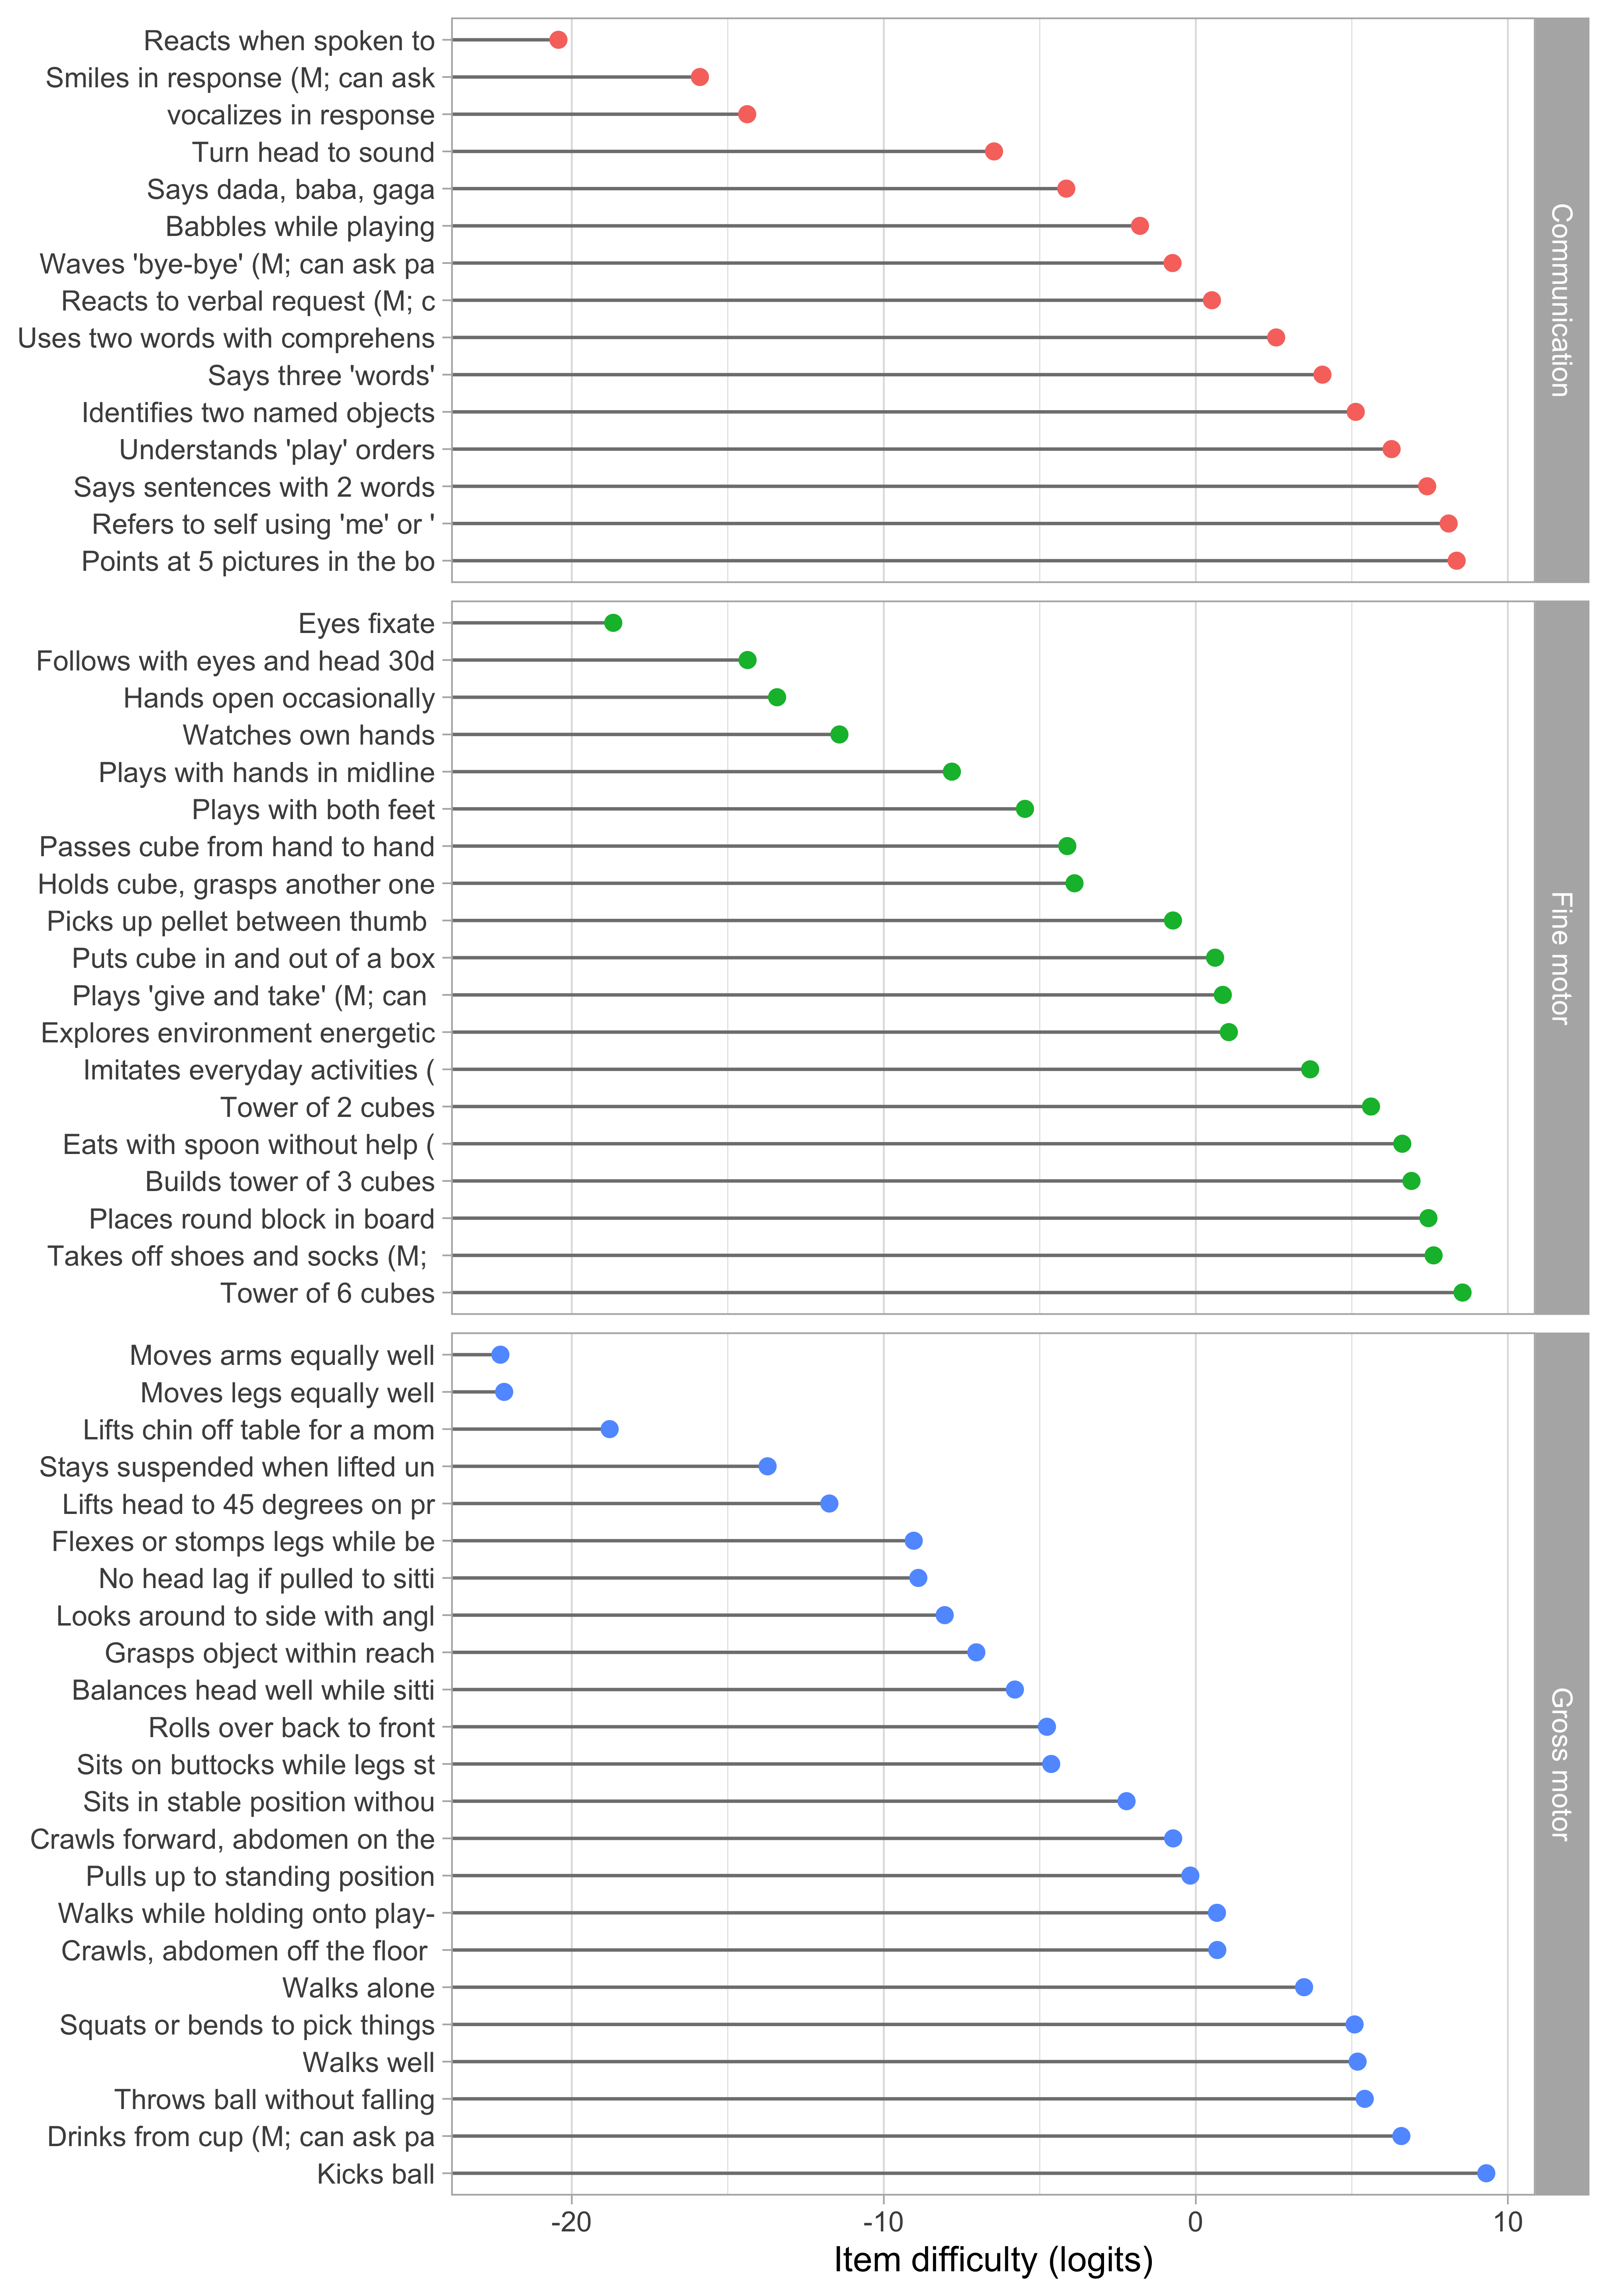
\includegraphics[width=1\linewidth]{dbook1_files/figure-latex/itemdiflplot-1} 

}

\caption{Estimated item difficulty parameters (\(d_i\)) for 57 milestones of the DDI (0 - 2 years).}\label{fig:itemdiflplot}
\end{figure}



Figure \ref{fig:itemdiflplot} summarizes the estimated item difficulty parameters. Although the model makes no distinction between domains, the results have been ordered to ease spotting of the natural progression of the milestones per domain. The figure also suggests that not all domain have equal representation across the scale. For example, there are no communication milestones around the logit of \(-10\).

\hypertarget{sec:anchoring}{%
\subsection{Anchoring}\label{sec:anchoring}}

The Rasch model identifies the item difficulties up to a linear transformation. By default, the software produces estimates in the logit scale (c.f. Figure \ref{fig:itemdiflplot}). The logit scale is inconvenient for two reasons:

\begin{itemize}
\tightlist
\item
  The logit scale has negative values. Negative values do not have a sensible interpretation in child development, and are likely to introduce errors in practice;
\item
  Both the zero in the logit scale, as well as its variance, depend on the sample used to calibrate the item difficulties.
\end{itemize}

Rescaling preserves the properties of the Rasch model. To make the scale independent of the specified sample, we transform the scale so that two items will always have the same value on the transformed scale. The choice of the two anchor items is essentially arbitrary, but they should correspond to milestones that are easy to measure with small error. In the sequel, we use the two milestones to anchor the D-score scale:

\begin{table}

\caption{\label{tab:anchor}Anchoring values used to identify the D-score scale}
\centering
\begin{tabular}[t]{>{}llr}
\toprule
Item & Label & Value\\
\midrule
\ttfamily{ddigmd057} & Lifts head to 45 degrees on prone position & 20\\
\ttfamily{ddigmd063} & Sits in stable position without support & 40\\
\bottomrule
\end{tabular}
\end{table}

~

With the choice of Table \ref{tab:anchor}, D-score values are approximately 0\(D\) around birth. At the age of 1 year, the score will around 50\(D\), so during the first year of life, one \(D\) unit corresponds to approximately a one-week interval. Figure \ref{fig:itemdifdplot} shows the difficulty estimates in the D-score scale.

\begin{figure}

{\centering 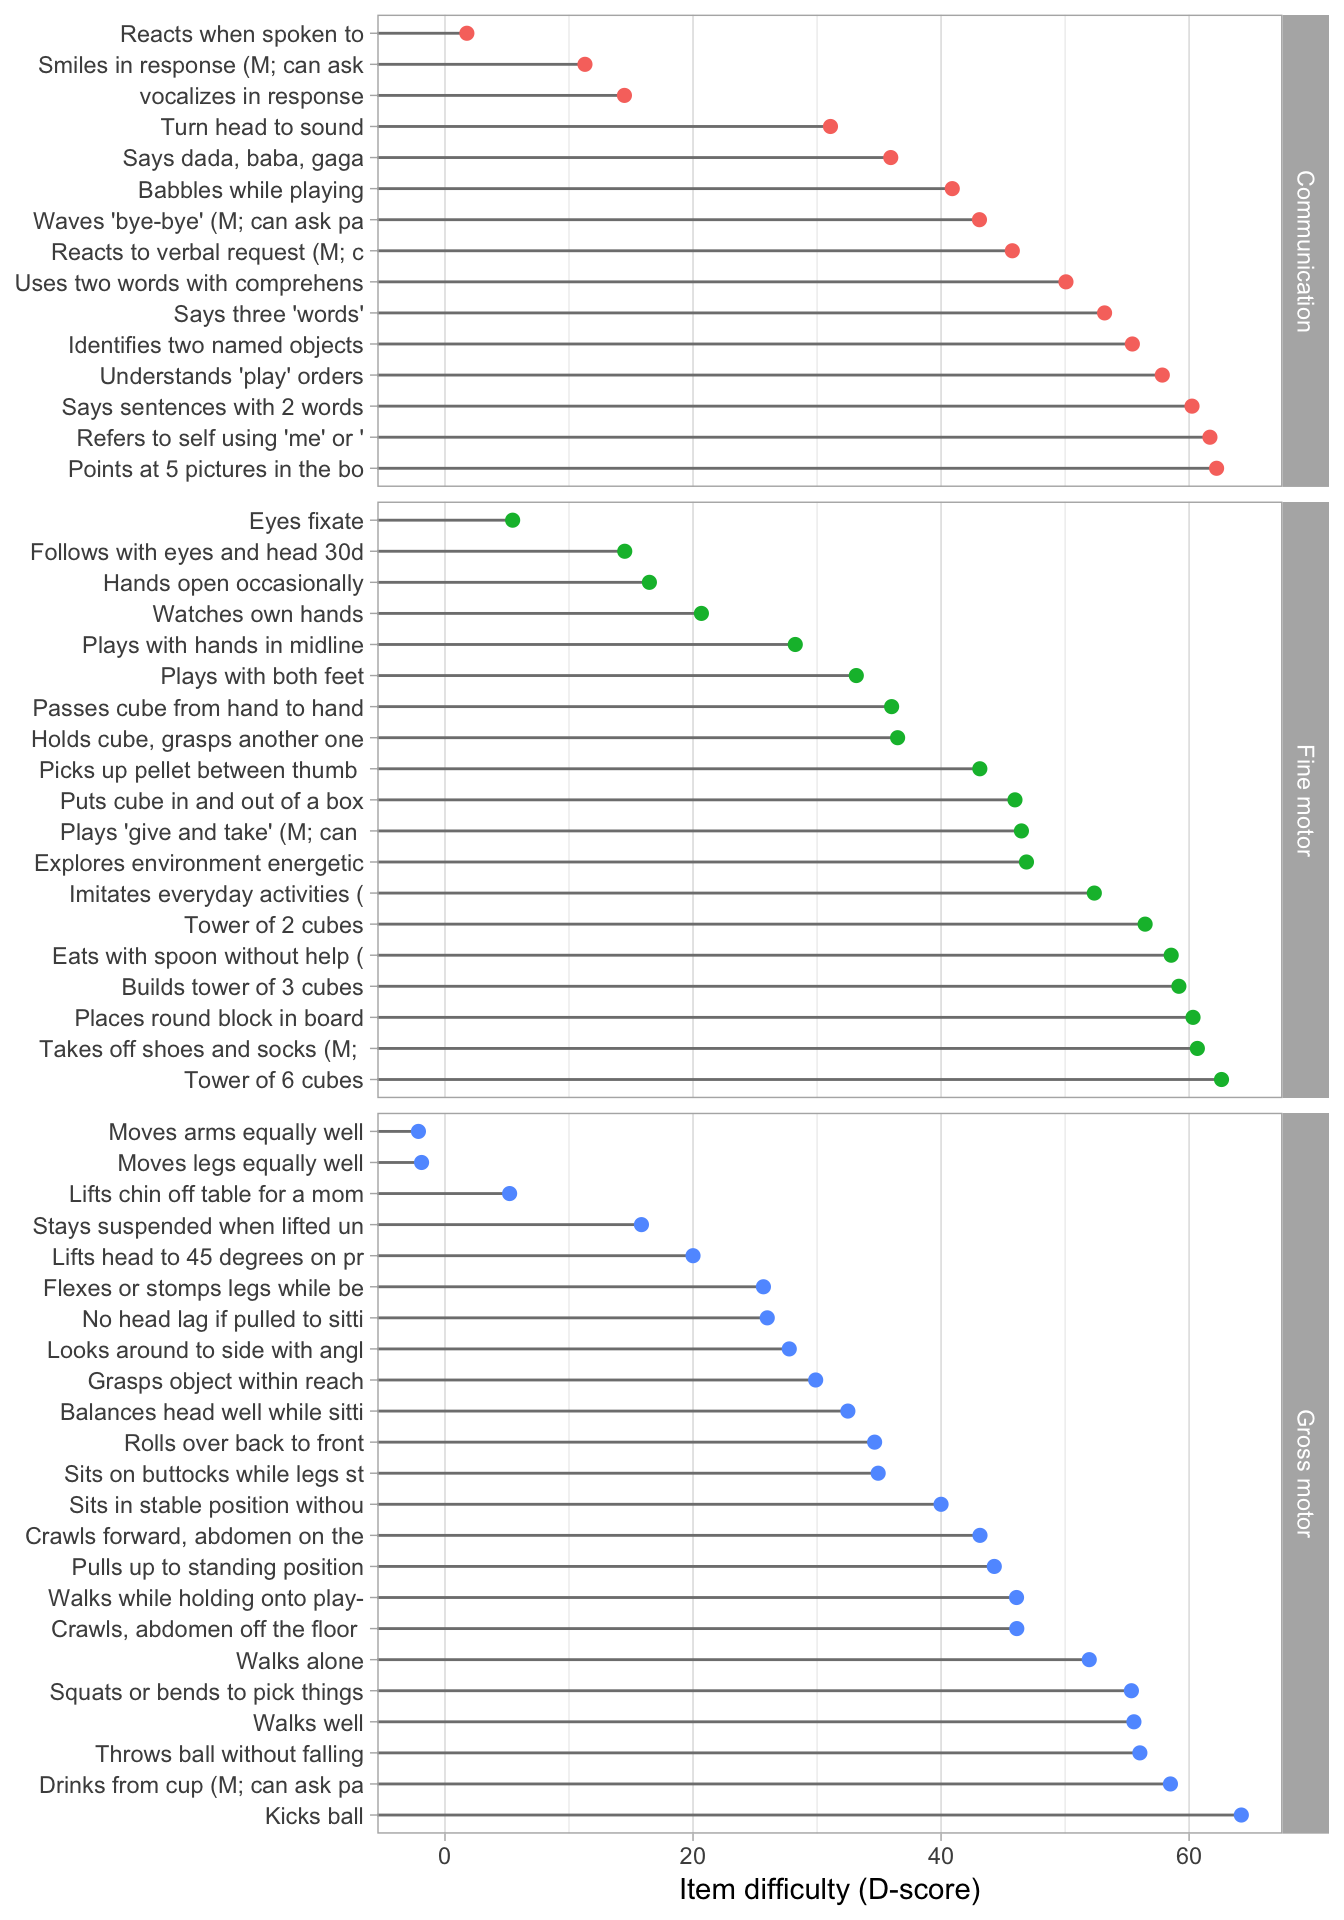
\includegraphics[width=1\linewidth]{dbook1_files/figure-latex/itemdifdplot-1} 

}

\caption{Estimated item difficulty parameters (\(d_i\)) for 57 milestones of the DDI (0 - 2 years). Milestones \texttt{ddigmd057} and \texttt{ddigmd063} are anchored at values of 20\(D\) and 40\(D\), respectively.}\label{fig:itemdifdplot}
\end{figure}



\hypertarget{sec:dscoreestimation}{%
\section{Estimation of the D-score}\label{sec:dscoreestimation}}

The second part of the estimation process is to estimate a D-score. The D-score quantifies the development of a child at a given age. Whereas the instrument developer is responsible for the estimation of item parameters, D-score estimation is more of a task for the user. To calculate the D-score, we need the following ingredients:

\begin{itemize}
\tightlist
\item
  Child's PASS/FAIL scores on the milestones administered;
\item
  The difficulty estimates of each milestone administered;
\item
  A prior distribution, an estimate of the D-score distribution before seeing any PASS/FAIL score.
\end{itemize}

Using these inputs, we may use Bayes theorem to calculate the position of the person on the latent variable.

\hypertarget{sec:startingprior}{%
\subsection{Role of the starting prior}\label{sec:startingprior}}

The first two inputs to the D-score will be self-evident. The third component, the prior distribution, is needed to be able to deal with perfect responses. The prior distribution summarizes our knowledge about the D-score before we see any of the child's PASS/FAIL scores. In general, we like the prior to be non-informative, so that the observed responses and item difficulties entirely determine the value of the D-score. In practice, we cannot use truly non-informative prior because that would leave the D-score for perfect responses (i.e., all PASS or all FAIL) undefined. The choice of the prior is essentially arbitrary, but we can make it in such a way that its impact on the value D-score is negligible, especially for tests where we have more than, say, four items.

Since we know that the D-score depends on age, a logical choice for the prior is to make it dependent on age. In particular, we will define the prior as a normal distribution equal to the expected mean in Figure \ref{fig:smoccda} at the child's age, and with a standard deviation that considerably higher than in Figure \ref{fig:smoccda}. Numerical example: the mean D-score at the age of 15 months is equal to 53.6\(D\). The standard deviation in Figure \ref{fig:smoccda} varies between 2.6\(D\) and 3.0\(D\), with an average of 2.9\(D\). After some experimentation, we found that using a value of 5.0\(D\) for the prior yields a good compromise between non-informativeness and robustness of D-score estimates for perfect patterns. The resulting starting prior for a child aged 15 months is thus \(N(53.6, 5)\).

The reader now probably wonders about a chicken-and-egg problem: To calculate the D-score, we need a prior, and to determine the prior we need the D-score. So how did we calculate the D-scores in Figure \ref{fig:smoccda}? The answer is that we first took at rougher prior, and calculated two temporary models in succession using the D-scores obtained after solution 1 to inform the prior before solution 2, and so on. It turned out that D-scores in Figure \ref{fig:smoccda} hardly changed after two steps, and so there we stopped.

\hypertarget{sec:adp}{%
\subsection{Starting prior: Numerical example}\label{sec:adp}}

\begin{figure}

{\centering 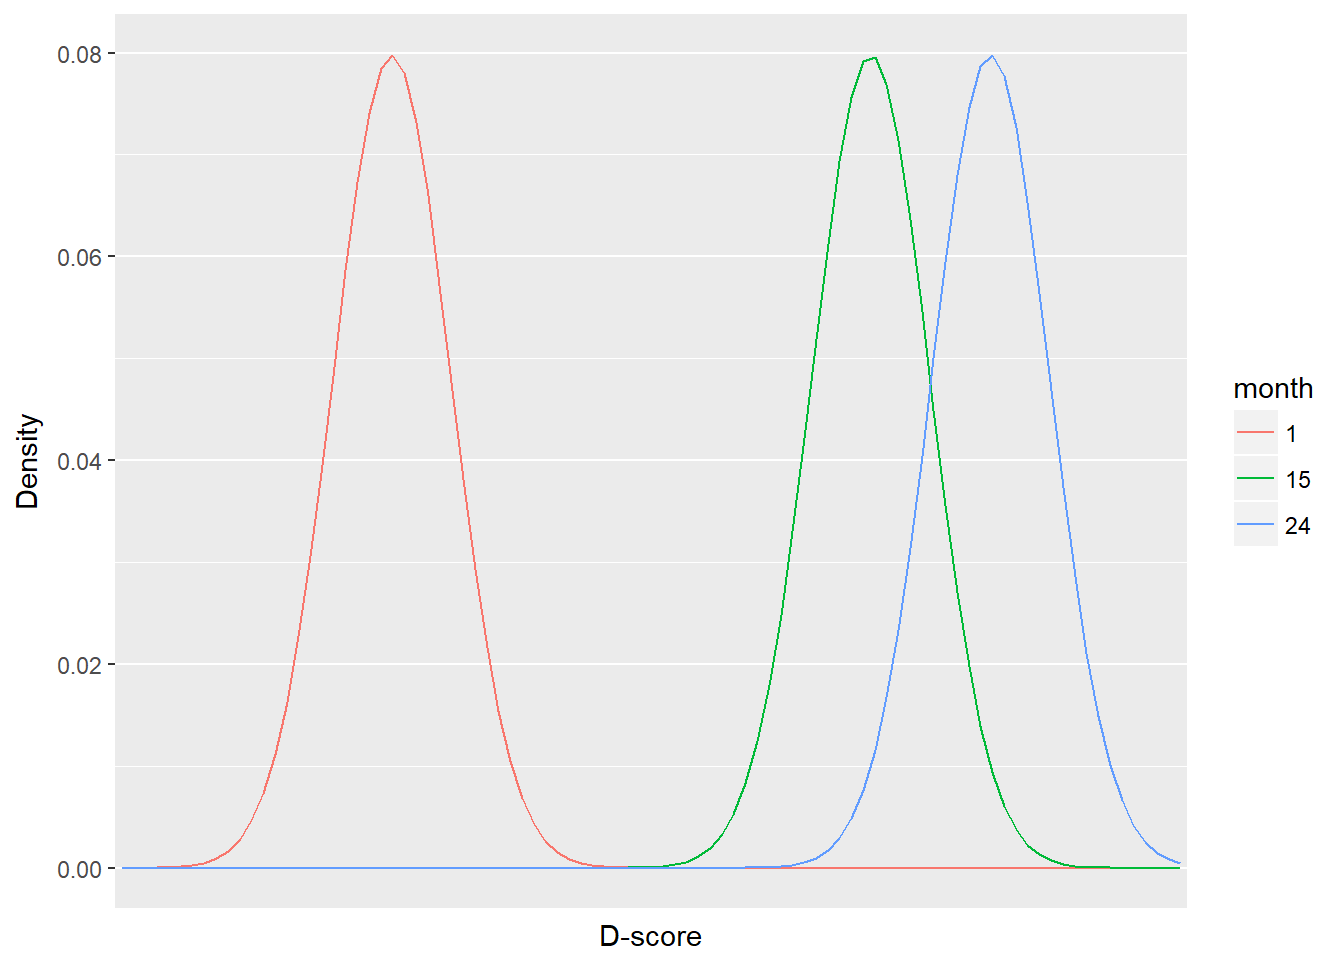
\includegraphics[width=1\linewidth]{dbook1_files/figure-latex/figpriors-1} 

}

\caption{Age-dependent starting priors for the D-score at the ages of 1, 15 and 24 months.}\label{fig:figpriors}
\end{figure}



Figure \ref{fig:figpriors} illustrates starting distributions (priors) chosen according to the principles set above for the ages of 1, 15 and 24 months. As expected, the assumed ability of an infant aged one month is much lower than that of a child aged 15 months, which in turn is lower than the ability of a toddler aged 24 months. The green distribution for 15 months corresponds to the normal distribution \(N(53.6, 5)\).

Another choice that we need to make is the grid of points on which we calculate the prior and posterior distributions. Figure \ref{fig:figpriors} uses a grid from -10\(D\) to +80\(D\), with a step size of 1\(D\). These are fixed \emph{quadrature points}, and there are 91 of them. While these quadrature points are sufficient to estimate D-score for ages up to 2.5 years, it is wise to extend the range for older children with higher D-scores.

\hypertarget{sec:EAP}{%
\subsection{EAP algorithm}\label{sec:EAP}}

The algorithm for estimating the D-score is known as the Expected a posteriori (EAP) method, first described by \protect\hyperlink{ref-bock1982}{Bock and Mislevy} (\protect\hyperlink{ref-bock1982}{1982}). Calculation of the D-score proceeds item by item. Suppose we have some vague and preliminary idea about the distribution of \(D\), the starting prior (c.f. section \ref{sec:startingprior}), based on age. The procedure uses Bayes rule to update this prior knowledge with data from the first item (using the child's FAIL/PASS score and the estimated item difficulty) to calculate the posterior. The next step uses this posterior as prior before processing the next item, and so on. The procedure stops when the item pool is exhausted. The order in which items enter does not matter for the result. The D-score is equal to the mean of the posterior calculated after the last question.

\hypertarget{eap-algorithm-numerical-example}{%
\subsection{EAP algorithm: Numerical example}\label{eap-algorithm-numerical-example}}

Suppose we measure two boys aged 15 months, David and Rob, by the DDI. David passes the first four milestones but does not complete the test. Rob completes the test but fails on two out of five items.

\begin{table}

\caption{\label{tab:datadavidandrob}Scores of David and Rob on five milestones from the DDI}
\centering
\resizebox{\linewidth}{!}{
\begin{tabular}[t]{>{}llrrr}
\toprule
Item & Label & Delta & David & Rob\\
\midrule
\ttfamily{ddifmd011} & Puts cube in and out of a box & 46.0 & 1 & 1\\
\ttfamily{ddifmm012} & Plays 'give and take' (M; can ask parents) & 46.5 & 1 & 0\\
\ttfamily{ddicmm037} & Uses two words with comprehension & 50.1 & 1 & 1\\
\ttfamily{ddigmm066} & Crawls, abdomen off the floor (M; can ask parents) & 46.1 & 1 & 1\\
\ttfamily{ddigmm067} & Walks while holding onto play-pen or furniture & 46.1 &  & 0\\
\bottomrule
\end{tabular}}
\end{table}

Table \ref{tab:datadavidandrob} shows the difficulty of each milestone (in the column labelled ``Delta''), and the responses of David and Rob for the standard five DDI milestones for the age of 15 months.

The mean D-score for Dutch children aged 15 months is 53.6\(D\), so the milestones are easy to pass at this age, with the most difficult is \texttt{ddicmm037}. David passed all milestones but has no score on the last. Rob fails on \texttt{ddifmm012} and \texttt{ddigmm067}. How do we calculate the D-score for David and Rob?

\begin{figure}

{\centering 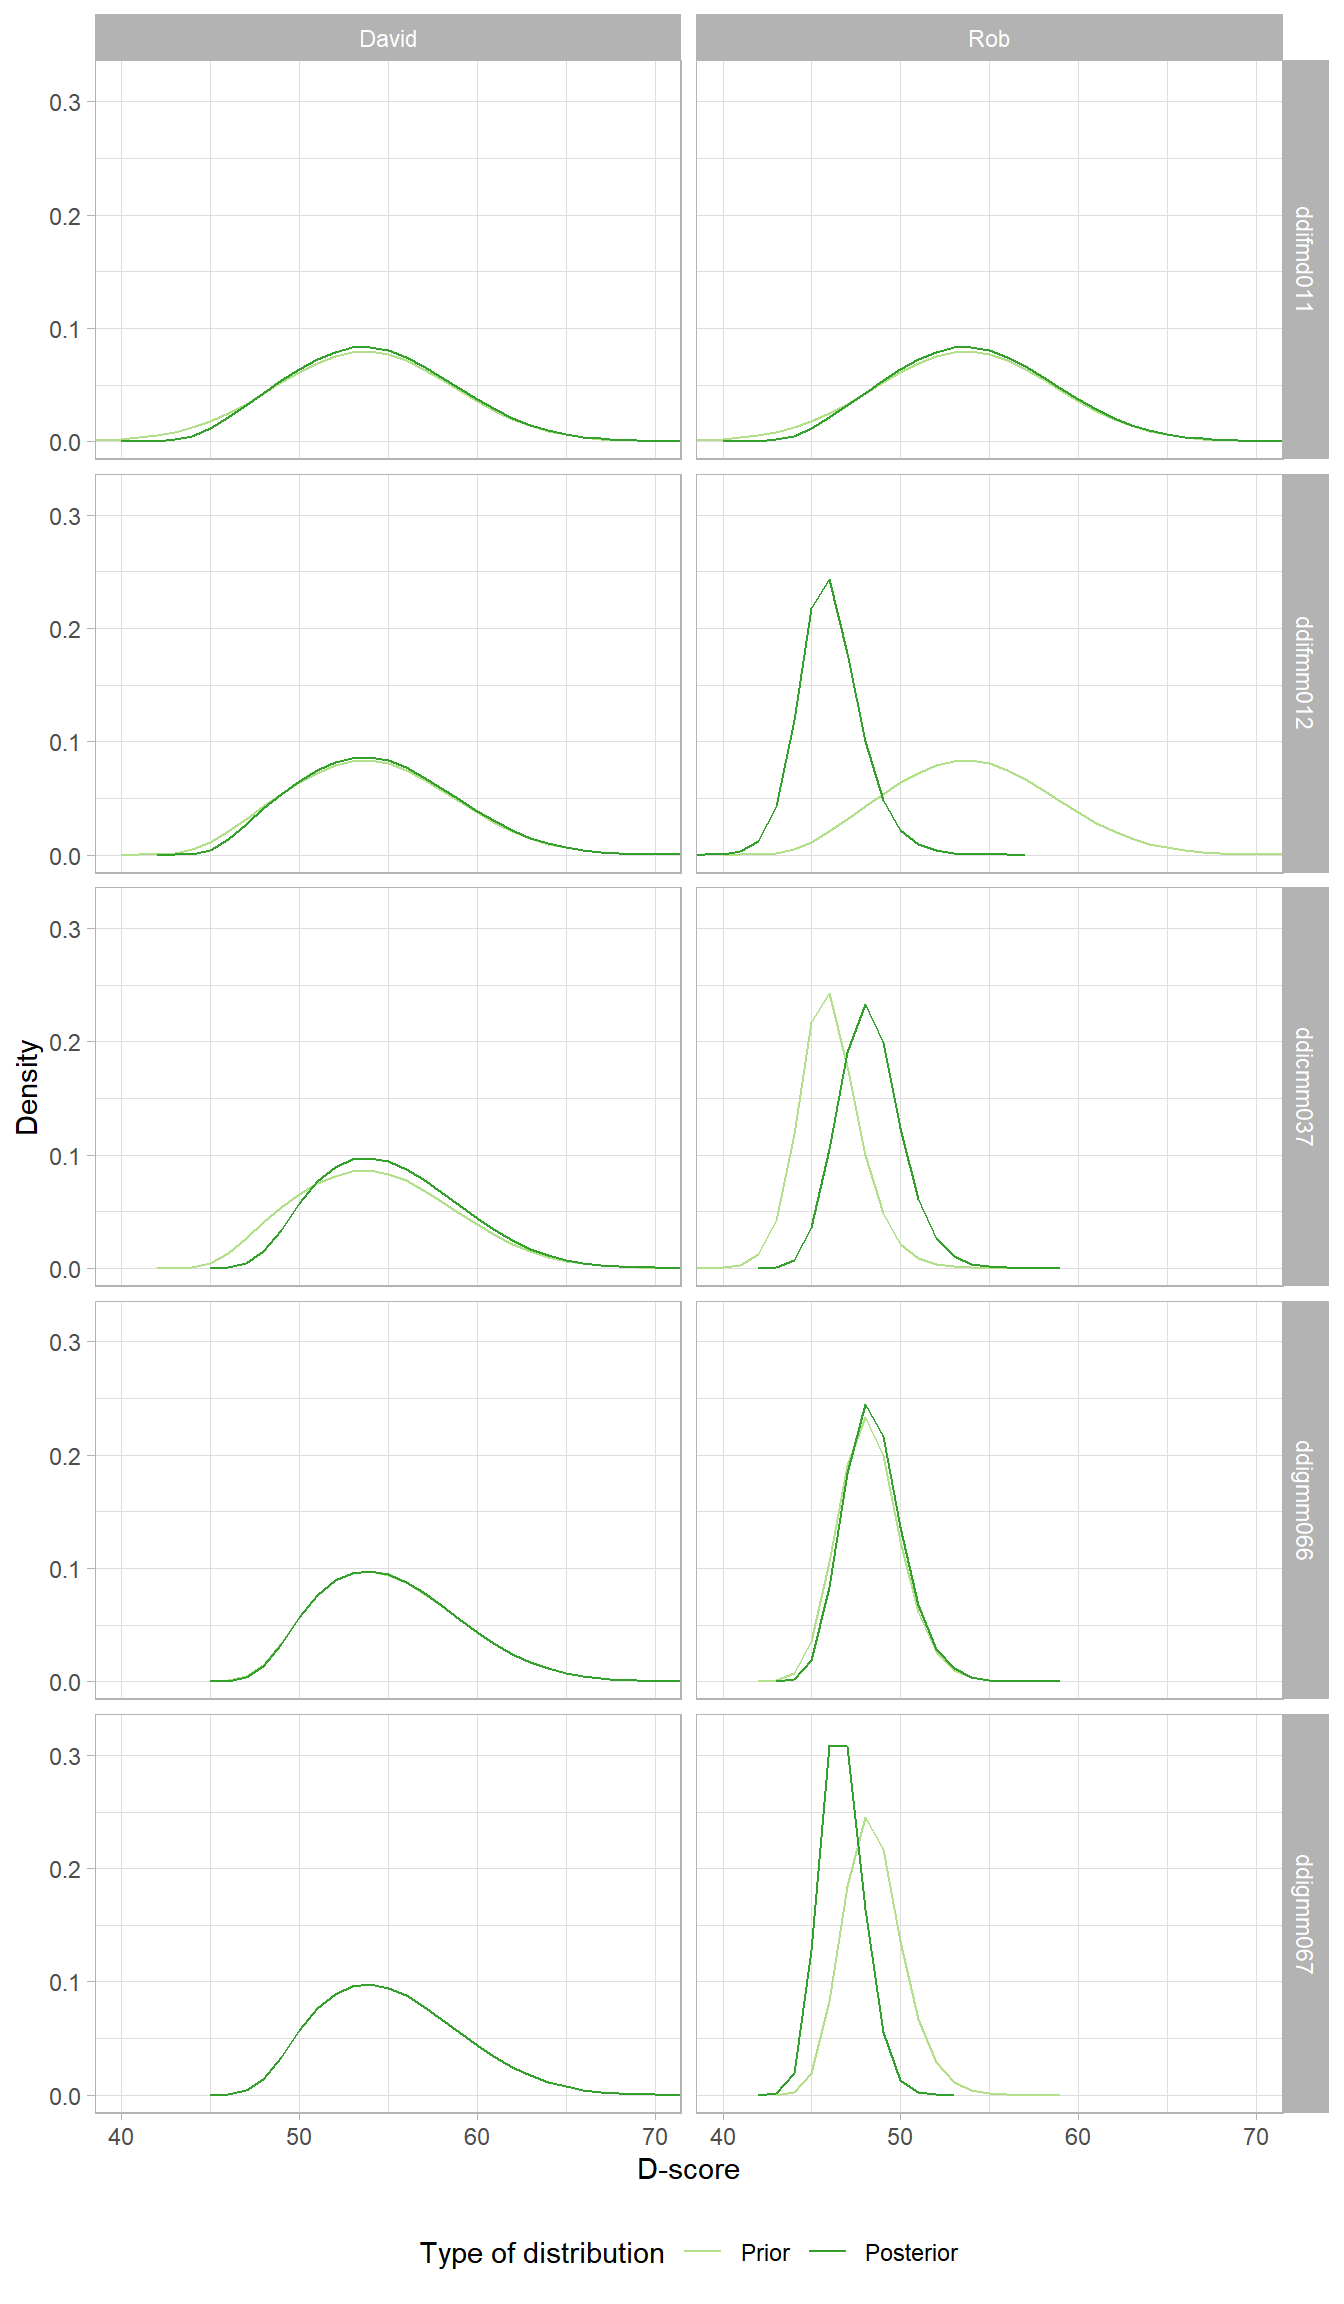
\includegraphics[width=1\linewidth]{dbook1_files/figure-latex/davidplot-1} 

}

\caption{D-score distribution for David and Rob before (prior) and after (posterior) a milestone is taken into account.}\label{fig:davidplot}
\end{figure}



Figure \ref{fig:davidplot} shows how the prior transforms into the posterior after we successively feed the measurements into the calculation. There are five milestones, so the calculation comprises five steps:

\begin{enumerate}
\def\labelenumi{\arabic{enumi}.}
\tightlist
\item
  Both David and Rob pass \texttt{ddifmd011}. The prior (light green) is the same as in Figure \ref{fig:figpriors}. After a PASS, the posterior will be located more to the right, and will often be more peaked. Both happen here, but the change is small. The reason is that a PASS on this milestone is not very informative. For a child with a true D-score of 53\(D\), the probability of passing \texttt{ddifmd011} is equal to 0.966. If passing is so common, there is not much information in the measurement.
\item
  David passes \texttt{ddifmm012}, but Rob does not. Observe that the prior is identical to the posterior of \texttt{ddifmd011}. For David, the posterior is only slightly different from the prior, for the same reason as above. For Rob, we find a considerable change to the left, both for location (from 54.3\(D\) to 47.1\(D\)) and peakedness. This one FAIL lowers Rob's score by 7.2\(D\).
\item
  Milestone \texttt{ddicmm037} is more difficult than the previous two milestones, so a pass on \texttt{ddicmm037} does have a definite effect on the posterior for both David and Rob.
\item
  David's PASS on \texttt{ddigmm066} does not bring any additional information, so his prior and posterior are virtually indistinguishable. For Rob, we find a slight shift to the right.
\item
  There is no measurement for David on \texttt{ddigmm067}, so the prior and posterior are equivalent. For Rob, we observe a FAIL, which shifts his posterior to the left.
\end{enumerate}

We calculate the D-score as the mean of the posterior. David's D-score is equal to 55.7\(D\). Note that the measurement error, as estimated from the variance of the posterior, is relatively large. Rob's D-score is equal to 47.7\(D\), with a much smaller measurement error. This result is consistent with the design principles of the DDI, which is meant to detect children with developmental delay.

The example illustrates that the quality of the D-score depends on two factors, the match between the true (but unknown) D-score of the child and the difficulty of the milestone.

\hypertarget{technical-observations-on-d-score-estimation}{%
\subsection{Technical observations on D-score estimation}\label{technical-observations-on-d-score-estimation}}

\begin{itemize}
\tightlist
\item
  Administration of a too easy set of milestones introduces a \emph{ceiling} with children that pass all milestones, but whose true D-score could extend well beyond the maximum. Depending on the goal of the measurement, this may or may not be a problem.
\item
  The specification of the prior and posterior distributions requires a set of quadrature points. The quadrature points are taken here as the static and evenly-spaced set of integers between -10 and +80. Using other quadrature points may affect the estimate, especially if the range of the quadrature points does not cover the entire D-score range.
\item
  The actual calculations are here done item by item. A more efficient method is to handle all responses at once. The result will be the same.
\end{itemize}

\hypertarget{sec:reference}{%
\section{Age-conditional references}\label{sec:reference}}

\hypertarget{motivation}{%
\subsection{Motivation}\label{motivation}}

The last step involves estimation an age-conditional reference distribution for the D-score. This distribution can be used to construct growth charts that portray the normal variation in development. Also, the references can be used to calculate age-standardized D-scores, called DAZ, that emphasize the location of the measurement in comparison to age peers.

Estimation of reference centiles is reasonably standard. Here we follow \protect\hyperlink{ref-vanbuuren2014}{van Buuren} (\protect\hyperlink{ref-vanbuuren2014}{2014}) to fit age-conditional references of the D-score for boys and girls combined by the LMS method. The LMS method by \protect\hyperlink{ref-cole1992}{Cole and Green} (\protect\hyperlink{ref-cole1992}{1992}) assumes that the outcome has a normal distribution after a Box-Cox transformation. The reference distribution has three parameters, which model respectively the location (\(M\)), the spread (\(S\)), and the skewness (\(L\)) of the distribution. Each of the three parameters can vary smoothly with age.

\hypertarget{estimation-of-the-reference-distribution}{%
\subsection{Estimation of the reference distribution}\label{estimation-of-the-reference-distribution}}

The parameters are estimated using the BCCG distribution of \texttt{gamlss\ 5.1-3} (\protect\hyperlink{ref-stasinopoulos2007}{Stasinopoulos and Rigby 2007}) using cubic splines smoothers. The final solution used a log-transformed age scale and fitted the model with smoothing parameters \(\mathrm{df}(M)=2\), \(\mathrm{df}(S)=2\) and \(\mathrm{df}(L)=1\).

Figure \ref{fig:smoccda} plots the D-scores together with five grey lines, corresponding to the centiles -2SD (P2), -1SD (P16), 0SD (P50), +1SD (P84) and +2SD (P98). The area between the -2SD and +2SD lines delineates the D-score expected if development is healthy. Note that the shape of the reference is quite similar to that of weight and height, with rapid growth occurring in the first few months.

\begin{longtabu} to \linewidth {>{}r>{\raggedleft}X>{\raggedleft}X>{\raggedleft}X}
\caption{\label{tab:reftable}Dutch reference values for the D-score: M-curve (median), S-curve (spread) and L-curve (skewness).}\\
\toprule
age & M & S & L\\
\midrule
\endfirsthead
\caption[]{\label{tab:reftable}Dutch reference values for the D-score: M-curve (median), S-curve (spread) and L-curve (skewness). \textit{(continued)}}\\
\toprule
age & M & S & L\\
\midrule
\endhead

\endfoot
\bottomrule
\endlastfoot
\ttfamily{0.0383} & 8.81 & 0.3126 & 1.3917\\
\ttfamily{0.0575} & 10.59 & 0.2801 & 1.4418\\
\ttfamily{0.0767} & 12.27 & 0.2526 & 1.4891\\
\ttfamily{0.0958} & 13.87 & 0.2291 & 1.5331\\
\ttfamily{0.1150} & 15.39 & 0.2089 & 1.5722\\
\addlinespace
\ttfamily{0.1342} & 16.83 & 0.1916 & 1.6049\\
\ttfamily{0.1533} & 18.20 & 0.1767 & 1.6304\\
\ttfamily{0.1725} & 19.50 & 0.1640 & 1.6487\\
\ttfamily{0.1916} & 20.75 & 0.1531 & 1.6607\\
\ttfamily{0.2108} & 21.94 & 0.1436 & 1.6676\\
\addlinespace
\ttfamily{0.2300} & 23.07 & 0.1354 & 1.6706\\
\ttfamily{0.2491} & 24.16 & 0.1283 & 1.6711\\
\ttfamily{0.2683} & 25.21 & 0.1220 & 1.6698\\
\ttfamily{0.2875} & 26.21 & 0.1165 & 1.6673\\
\ttfamily{0.3066} & 27.17 & 0.1117 & 1.6636\\
\addlinespace
\ttfamily{0.3258} & 28.10 & 0.1074 & 1.6589\\
\ttfamily{0.3450} & 28.99 & 0.1035 & 1.6533\\
\ttfamily{0.3641} & 29.86 & 0.1001 & 1.6471\\
\ttfamily{0.3833} & 30.70 & 0.0970 & 1.6403\\
\ttfamily{0.4025} & 31.50 & 0.0942 & 1.6330\\
\addlinespace
\ttfamily{0.4216} & 32.29 & 0.0917 & 1.6255\\
\ttfamily{0.4408} & 33.05 & 0.0894 & 1.6178\\
\ttfamily{0.4600} & 33.79 & 0.0873 & 1.6100\\
\ttfamily{0.4791} & 34.51 & 0.0854 & 1.6022\\
\ttfamily{0.4983} & 35.21 & 0.0837 & 1.5946\\
\addlinespace
\ttfamily{0.5175} & 35.89 & 0.0821 & 1.5870\\
\ttfamily{0.5366} & 36.55 & 0.0807 & 1.5797\\
\ttfamily{0.5558} & 37.20 & 0.0793 & 1.5725\\
\ttfamily{0.5749} & 37.83 & 0.0781 & 1.5656\\
\ttfamily{0.5941} & 38.44 & 0.0770 & 1.5588\\
\addlinespace
\ttfamily{0.6133} & 39.04 & 0.0759 & 1.5523\\
\ttfamily{0.6324} & 39.63 & 0.0749 & 1.5460\\
\ttfamily{0.6516} & 40.21 & 0.0740 & 1.5399\\
\ttfamily{0.6708} & 40.77 & 0.0731 & 1.5340\\
\ttfamily{0.6899} & 41.32 & 0.0723 & 1.5284\\
\addlinespace
\ttfamily{0.7091} & 41.86 & 0.0715 & 1.5230\\
\ttfamily{0.7283} & 42.39 & 0.0707 & 1.5178\\
\ttfamily{0.7474} & 42.91 & 0.0700 & 1.5128\\
\ttfamily{0.7666} & 43.42 & 0.0693 & 1.5081\\
\ttfamily{0.7858} & 43.92 & 0.0687 & 1.5036\\
\addlinespace
\ttfamily{0.8049} & 44.40 & 0.0681 & 1.4993\\
\ttfamily{0.8241} & 44.88 & 0.0674 & 1.4952\\
\ttfamily{0.8433} & 45.36 & 0.0669 & 1.4913\\
\ttfamily{0.8624} & 45.82 & 0.0663 & 1.4876\\
\ttfamily{0.8816} & 46.27 & 0.0657 & 1.4841\\
\addlinespace
\ttfamily{0.9008} & 46.72 & 0.0652 & 1.4809\\
\ttfamily{0.9199} & 47.16 & 0.0647 & 1.4778\\
\ttfamily{0.9391} & 47.59 & 0.0642 & 1.4749\\
\ttfamily{0.9582} & 48.01 & 0.0637 & 1.4723\\
\ttfamily{0.9774} & 48.43 & 0.0632 & 1.4698\\
\addlinespace
\ttfamily{0.9966} & 48.84 & 0.0627 & 1.4676\\
\ttfamily{1.0157} & 49.24 & 0.0622 & 1.4655\\
\ttfamily{1.0349} & 49.64 & 0.0618 & 1.4637\\
\ttfamily{1.0541} & 50.03 & 0.0613 & 1.4620\\
\ttfamily{1.0732} & 50.41 & 0.0608 & 1.4605\\
\addlinespace
\ttfamily{1.0924} & 50.79 & 0.0604 & 1.4592\\
\ttfamily{1.1116} & 51.16 & 0.0600 & 1.4580\\
\ttfamily{1.1307} & 51.53 & 0.0595 & 1.4570\\
\ttfamily{1.1499} & 51.89 & 0.0591 & 1.4561\\
\ttfamily{1.1691} & 52.24 & 0.0587 & 1.4553\\
\addlinespace
\ttfamily{1.1882} & 52.59 & 0.0583 & 1.4547\\
\ttfamily{1.2074} & 52.94 & 0.0578 & 1.4542\\
\ttfamily{1.2266} & 53.27 & 0.0574 & 1.4538\\
\ttfamily{1.2457} & 53.61 & 0.0570 & 1.4535\\
\ttfamily{1.2649} & 53.94 & 0.0566 & 1.4534\\
\addlinespace
\ttfamily{1.2841} & 54.26 & 0.0562 & 1.4533\\
\ttfamily{1.3032} & 54.58 & 0.0559 & 1.4533\\
\ttfamily{1.3224} & 54.89 & 0.0555 & 1.4533\\
\ttfamily{1.3415} & 55.20 & 0.0551 & 1.4535\\
\ttfamily{1.3607} & 55.50 & 0.0547 & 1.4537\\
\addlinespace
\ttfamily{1.3799} & 55.81 & 0.0544 & 1.4539\\
\ttfamily{1.3990} & 56.10 & 0.0540 & 1.4542\\
\ttfamily{1.4182} & 56.39 & 0.0536 & 1.4546\\
\ttfamily{1.4374} & 56.68 & 0.0533 & 1.4551\\
\ttfamily{1.4565} & 56.97 & 0.0530 & 1.4555\\
\addlinespace
\ttfamily{1.4757} & 57.25 & 0.0526 & 1.4561\\
\ttfamily{1.4949} & 57.52 & 0.0523 & 1.4567\\
\ttfamily{1.5140} & 57.80 & 0.0520 & 1.4573\\
\ttfamily{1.5332} & 58.06 & 0.0517 & 1.4580\\
\ttfamily{1.5524} & 58.33 & 0.0514 & 1.4587\\
\addlinespace
\ttfamily{1.5715} & 58.59 & 0.0510 & 1.4595\\
\ttfamily{1.5907} & 58.85 & 0.0508 & 1.4603\\
\ttfamily{1.6099} & 59.11 & 0.0505 & 1.4612\\
\ttfamily{1.6290} & 59.36 & 0.0502 & 1.4620\\
\ttfamily{1.6482} & 59.61 & 0.0499 & 1.4630\\
\addlinespace
\ttfamily{1.6674} & 59.86 & 0.0496 & 1.4639\\
\ttfamily{1.6865} & 60.11 & 0.0494 & 1.4649\\
\ttfamily{1.7057} & 60.35 & 0.0491 & 1.4660\\
\ttfamily{1.7248} & 60.59 & 0.0488 & 1.4670\\
\ttfamily{1.7440} & 60.82 & 0.0486 & 1.4681\\
\addlinespace
\ttfamily{1.7632} & 61.06 & 0.0483 & 1.4692\\
\ttfamily{1.7823} & 61.29 & 0.0481 & 1.4704\\
\ttfamily{1.8015} & 61.52 & 0.0478 & 1.4716\\
\ttfamily{1.8207} & 61.75 & 0.0476 & 1.4728\\
\ttfamily{1.8398} & 61.97 & 0.0474 & 1.4740\\
\addlinespace
\ttfamily{1.8590} & 62.20 & 0.0471 & 1.4752\\
\ttfamily{1.8782} & 62.42 & 0.0469 & 1.4765\\
\ttfamily{1.8973} & 62.64 & 0.0467 & 1.4778\\
\ttfamily{1.9165} & 62.85 & 0.0465 & 1.4791\\
\ttfamily{1.9357} & 63.07 & 0.0463 & 1.4805\\
\addlinespace
\ttfamily{1.9548} & 63.28 & 0.0461 & 1.4818\\
\ttfamily{1.9740} & 63.49 & 0.0459 & 1.4832\\
\ttfamily{1.9932} & 63.70 & 0.0457 & 1.4846\\
\ttfamily{2.0123} & 63.91 & 0.0455 & 1.4861\\
\ttfamily{2.0315} & 64.11 & 0.0453 & 1.4875\\
\addlinespace
\ttfamily{2.0507} & 64.32 & 0.0451 & 1.4890\\
\ttfamily{2.0698} & 64.52 & 0.0449 & 1.4904\\
\ttfamily{2.0890} & 64.72 & 0.0447 & 1.4919\\
\ttfamily{2.1081} & 64.92 & 0.0445 & 1.4934\\
\ttfamily{2.1273} & 65.11 & 0.0443 & 1.4949\\
\addlinespace
\ttfamily{2.1465} & 65.31 & 0.0441 & 1.4964\\
\ttfamily{2.1656} & 65.50 & 0.0440 & 1.4979\\
\ttfamily{2.1848} & 65.70 & 0.0438 & 1.4994\\
\ttfamily{2.2040} & 65.89 & 0.0436 & 1.5009\\
\ttfamily{2.2231} & 66.08 & 0.0434 & 1.5024\\
\addlinespace
\ttfamily{2.2423} & 66.26 & 0.0433 & 1.5039\\
\ttfamily{2.2615} & 66.45 & 0.0431 & 1.5054\\
\ttfamily{2.2806} & 66.64 & 0.0429 & 1.5069\\
\ttfamily{2.2998} & 66.82 & 0.0428 & 1.5084\\
\ttfamily{2.3190} & 67.00 & 0.0426 & 1.5098\\
\addlinespace
\ttfamily{2.3381} & 67.18 & 0.0425 & 1.5113\\
\ttfamily{2.3573} & 67.36 & 0.0423 & 1.5127\\
\ttfamily{2.3765} & 67.54 & 0.0421 & 1.5142\\
\ttfamily{2.3956} & 67.72 & 0.0420 & 1.5156\\
\ttfamily{2.4148} & 67.89 & 0.0418 & 1.5170\\
\addlinespace
\ttfamily{2.4339} & 68.07 & 0.0417 & 1.5185\\
\ttfamily{2.4531} & 68.24 & 0.0415 & 1.5199\\
\ttfamily{2.4723} & 68.41 & 0.0414 & 1.5213\\
\ttfamily{2.4914} & 68.59 & 0.0412 & 1.5226\\
\ttfamily{2.5106} & 68.75 & 0.0411 & 1.5240\\
\addlinespace
\ttfamily{2.5298} & 68.92 & 0.0410 & 1.5254\\
\ttfamily{2.5489} & 69.09 & 0.0408 & 1.5267\\
\ttfamily{2.5681} & 69.26 & 0.0407 & 1.5281\\
\ttfamily{2.5873} & 69.42 & 0.0405 & 1.5294\\
\ttfamily{2.6064} & 69.59 & 0.0404 & 1.5308\\
\addlinespace
\ttfamily{2.6256} & 69.75 & 0.0403 & 1.5321\\
\ttfamily{2.6448} & 69.91 & 0.0401 & 1.5334\\
\ttfamily{2.6639} & 70.07 & 0.0400 & 1.5347\\
\ttfamily{2.6831} & 70.23 & 0.0399 & 1.5360\\
\ttfamily{2.7023} & 70.39 & 0.0397 & 1.5373\\
\addlinespace
\ttfamily{2.7214} & 70.55 & 0.0396 & 1.5386\\
\ttfamily{2.7406} & 70.71 & 0.0395 & 1.5398\\
\ttfamily{2.7598} & 70.86 & 0.0394 & 1.5411\\
\ttfamily{2.7789} & 71.02 & 0.0392 & 1.5423\\*
\end{longtabu}

Table \ref{tab:reftable} defines age-conditional references for Dutch children as the \(M\)-curve (median), \(S\)-curve (spread) and \(L\)-curve (skewness) by age. This table can be used to calculate centile lines and \(Z\)-scores.

The references are purely cross-sectional and do not account for the correlation structure between ages. For prediction purposes, it is useful to extend the modelling to include velocities and change scores.

\hypertarget{conversion-of-d-to-daz-and-vice-versa}{%
\subsection{\texorpdfstring{Conversion of \(D\) to DAZ, and vice versa}{Conversion of D to DAZ, and vice versa}}\label{conversion-of-d-to-daz-and-vice-versa}}

Suppose that \(M_t\), \(S_t\) and \(L_t\) are the parameter values at age \(t\). \protect\hyperlink{ref-cole1988}{Cole} (\protect\hyperlink{ref-cole1988}{1988}) shows that the transformation

\[Z=\frac{(D_t/M_t)^{L_t}-1}{L_t S_t}\]

converts measurement \(D_t\) into its normal equivalent deviate \(Z\). If \(L_t\) is close to zero, we use

\[Z=\frac{\ln(D_t/M_t)}{S_t}\]

We may derive any required centile curve from Table \ref{tab:reftable}. First, choose \(Z_\alpha\) as the \(Z\)-score that delineates \(100\alpha\) per cent of the distribution, for example, ~\(Z_{0.05}=-1.64\). The D-score that defines the \(100\alpha\) centile is equal to

\[D_t(\alpha) = M_t (1+L_t S_t Z_\alpha)^{1/L_t}\]

If \(L_t\) is close to zero, we use

\[D_t(\alpha)= M_t \exp(S_t Z_\alpha).\]

\hypertarget{references}{%
\chapter*{References}\label{references}}
\addcontentsline{toc}{chapter}{References}

\hypertarget{refs}{}
\begin{CSLReferences}{1}{0}
\leavevmode\hypertarget{ref-andrich1978}{}%
Andrich, D. 1978. {``A Rating Formulation for Ordered Response Categories.''} \emph{Psychometrika} 43: 561--73.

\leavevmode\hypertarget{ref-berk2013}{}%
Berk, L. E. 2011. \emph{Child Development. 9th Ed.} Boston, MA: Pearson.

\leavevmode\hypertarget{ref-berkson1944}{}%
Berkson, Joseph. 1944. {``Application of the Logistic Function to Bio-Assay.''} \emph{Journal of the American Statistical Association} 39 (227): 357--65. \url{http://www.jstor.org/stable/2280041}.

\leavevmode\hypertarget{ref-bock1982}{}%
Bock, D. D., and R. J. Mislevy. 1982. {``Adaptive {EAP} Estimation of Ability in a Microcomputer Environment.''} \emph{Applied Psychological Measurement} 6 (4): 431--44.

\leavevmode\hypertarget{ref-cameron2012}{}%
Cameron, N., and B. Bogin. 2012. \emph{Human Growth and Development}. London: Academic Press.

\leavevmode\hypertarget{ref-cole1988}{}%
Cole, T. J. 1988. {``Fitting Smoothed Centile Curves to Reference Data (with Discussion).''} \emph{Journal of the Royal Statistical Society, Series A} 151: 385--418.

\leavevmode\hypertarget{ref-cole1992}{}%
Cole, T. J., and P. J. Green. 1992. {``Smoothing Reference Centile Curves: The {LMS} Method and Penalized Likelihood.''} \emph{Statistics in Medicine} 11 (10): 1305--19.

\leavevmode\hypertarget{ref-coombs1964}{}%
Coombs, C. H. 1964. \emph{A Theory of Data}. New York: Wiley.

\leavevmode\hypertarget{ref-embretsen2000}{}%
Embretsen, S. E., and S. P. Reise. 2000. \emph{Item Response Theory for Psychologists}. Mahwah, NJ: Lawrence Erlbaum.

\leavevmode\hypertarget{ref-engelhard2013}{}%
Engelhard Jr., G. 2013. \emph{Invariant Measurement}. New York: Routledge.

\leavevmode\hypertarget{ref-erikson1963}{}%
Erikson, E. H. 1963. \emph{Childhood and Society. 2d Ed., Rev. And Enl}. New York, NJ: Norton.

\leavevmode\hypertarget{ref-frankenburg1992}{}%
Frankenburg, W. K., J. Dodds, P. Archer, H. Shapiro, and B. Bresnick. 1992. {``The Denver II: A Major Revision and Restandardization of the Denver Developmental Screening Test.''} \emph{Pediatrics} 89 (1): 91--97.

\leavevmode\hypertarget{ref-gesell1943}{}%
Gesell, A. 1943. \emph{Infant and Child in the Culture of Today}. Los Angeles, CA: Read Book Ltd.

\leavevmode\hypertarget{ref-guttman1950}{}%
Guttman, L. 1950. {``The Basis for Scalogram Snalysis.''} In \emph{Measurement and Prediction, Vol. IV}, edited by S. A. Stouffer, L. Guttman, E. A. Suchman, P. F. Lazarsfeld, S. A. Star, and J. A. Clausen, 60--90. Princeton, NJ: Princeton University Press.

\leavevmode\hypertarget{ref-hattie1985}{}%
Hattie, J. 1985. {``Methodology Review: Assessing Unidimensionality of Tests and Items.''} \emph{Applied Psychological Measurement} 9 (2): 139--64.

\leavevmode\hypertarget{ref-herngreen1994}{}%
Herngreen, W. P., S. van Buuren, J. C. van Wieringen, J. D. Reerink, S. P. Verloove-Vanhorick, and J. H. Ruys. 1994. {``Growth in Length and Weight from Birth to 2 Years of a Representative Sample of Netherlands Children (born in 1988-89) Related to Socio-Economic Status and Other Background Characteristics.''} \emph{Annals of Human Biology} 21 (5): 449--63.

\leavevmode\hypertarget{ref-jacobusse2007}{}%
Jacobusse, G., and S. van Buuren. 2007. {``Computerized Adaptive Testing for Measuring Development of Young Children.''} \emph{Statistics in Medicine} 26 (13): 2629--38. \url{https://stefvanbuuren.name/publication/2007-01-01_jacobusse2007/}.

\leavevmode\hypertarget{ref-jacobusse2006}{}%
Jacobusse, G., S. van Buuren, and P. H. Verkerk. 2006. {``An Interval Scale for Development of Children Aged 0-2 Years.''} \emph{Statistics in Medicine} 25 (13): 2272--83. \url{https://stefvanbuuren.name/publication/2006-01-01_jacobusse2006/}.

\leavevmode\hypertarget{ref-kohlberg1984}{}%
Kohlberg, L. 1984. \emph{The Psychology of Moral Development: The Nature and Validity of Moral Stages: Vol.~2}. San Francisco: Harpen \& Row.

\leavevmode\hypertarget{ref-liebert1974}{}%
Liebert, R. M., R. W. Poulos, and G. D. Strauss. 1974. \emph{Developmental Psychology}. Englewood Cliffs, NJ: Prentice-Hall, Inc.

\leavevmode\hypertarget{ref-linacre2004}{}%
Linacre, J. M. 2004. {``Rasch Model Estimation: Further Topics.''} \emph{Journal of Applied Measurement} 5 (1): 95--110.

\leavevmode\hypertarget{ref-mokken1971}{}%
Mokken, R. J. 1971. \emph{A Theory and Procedure of Scale Analysis: With Applications in Political Research}. Berlin: Walter de Gruyter.

\leavevmode\hypertarget{ref-molenaar1997}{}%
Molenaar, I. W. 1997. {``Nonparametric Models for Polytomous Responses.''} In \emph{Handbook of Modern Item Response Theory}, 369--80. Springer.

\leavevmode\hypertarget{ref-piaget1969}{}%
Piaget, J., and B. Inhelder. 1969. \emph{The Psychology of the Child}. New York, NJ: Basic Books.

\leavevmode\hypertarget{ref-rasch1960}{}%
Rasch, G. 1960. \emph{Probabilistic Models for Some Intelligence and Attainment Tests}. Copenhagen: Danish Institute for Educational Research.

\leavevmode\hypertarget{ref-rasch1977}{}%
---------. 1977. {``On Specific Objectivity: An Attempt at Formalizing the Request for Generality and Validity of Scientific Statements.''} \emph{The Danish Yearbook of Philosophy} 14: 58--93. \url{https://www.rasch.org/memo18.htm}.

\leavevmode\hypertarget{ref-robitzsch2016}{}%
Robitzsch, A. 2016. \emph{Sirt: Supplementary Item Response Theory Models}. \url{https://CRAN.R-project.org/package=sirt}.

\leavevmode\hypertarget{ref-salkind2002}{}%
Salkind, N. J., ed. 2002. \emph{Child Development}. Macmillan Library Reference.

\leavevmode\hypertarget{ref-santrock2010}{}%
Santrock, J. 2011. \emph{Child Development: An Introduction. 13th Ed.} New York, NJ: McGraw-Hill Higher Education.

\leavevmode\hypertarget{ref-shirley1931}{}%
Shirley, M. M. 1931. \emph{The First Two Years: A Study of Twenty-Five Babies}. Vol. I: Postural and Locomotor Development. Minneapolis: University of Minnesota Press.

\leavevmode\hypertarget{ref-shirley1933}{}%
---------. 1933. \emph{The First Two Years: A Study of Twenty-Five Babies}. Vol. II: Intellectual Development. Minneapolis: University of Minnesota Press.

\leavevmode\hypertarget{ref-stasinopoulos2007}{}%
Stasinopoulos, D., and R. Rigby. 2007. {``Generalized Additive Models for Location Scale and Shape ({GAMLSS}) in r.''} \emph{Journal of Statistical Software} 23 (7): 1--46. \url{https://doi.org/10.18637/jss.v023.i07}.

\leavevmode\hypertarget{ref-stott1967}{}%
Stott, L. H. 1967. \emph{Child Development: {A}n Individual Longitudinal Approach}. New York, NJ: Holt, Rinehart; Winston, Inc.

\leavevmode\hypertarget{ref-vanbuuren2014}{}%
van Buuren, S. 2014. {``Growth Charts of Human Development.''} \emph{Statistical Methods in Medical Research} 23 (4): 346--68. \url{https://stefvanbuuren.name/publication/2014-01-01_vanbuuren2014gc/}.

\leavevmode\hypertarget{ref-wright1982}{}%
Wright, B. D., and G. N. Masters. 1982. \emph{Rating Scale Analysis: Rasch Measurement}. Chicago: MESA Press.

\leavevmode\hypertarget{ref-zwinderman1995}{}%
Zwinderman, A. H. 1995. {``Pairwise Estimation in the Rasch Models.''} \emph{Applied Psychological Measurement} 19 (4): 369--75.

\end{CSLReferences}

\end{document}
